\documentclass[12pt,a4paper]{report}

%==============================================================================
% PREAMBLE AND PACKAGES (Aligned with CEK / KTU B.Tech Project Format)
%==============================================================================
\usepackage{graphicx}
\usepackage{amsmath}
\usepackage{fancyhdr}
\usepackage{cite}
\usepackage{a4wide}
\usepackage{float}
\usepackage{epsfig}
\usepackage{longtable}
\usepackage{enumerate}
\usepackage{afterpage}
\usepackage{multirow}
\usepackage{ragged2e}
\usepackage{gensymb}
\usepackage{amsfonts} 
\usepackage[left=3.5cm,top=1.5cm,right=3cm,bottom=3cm]{geometry}
\usepackage{setspace}           
\usepackage{txfonts}
\usepackage{standalone}
\usepackage{tikz}
\usepackage{fontawesome5}
\usetikzlibrary{calc, shapes.geometric, arrows, arrows.meta, positioning, fit, backgrounds, shadows, tikzmark}

% Color definitions for TikZ diagrams (Clinical Deep Navy, Ocean Blue & Cyan Palette)
\definecolor{lavenderDark}{RGB}{15, 44, 89}
\definecolor{lavenderDeep}{RGB}{10, 28, 58}
\definecolor{lavenderMedium}{RGB}{29, 78, 158}
\definecolor{lavenderLight}{RGB}{240, 246, 255}
\definecolor{lavenderBorder}{RGB}{180, 205, 237}
\definecolor{lavenderAccent}{RGB}{2, 132, 199}
\definecolor{prismNavy}{RGB}{15, 44, 89}
\definecolor{prismBlue}{RGB}{29, 78, 158}
\definecolor{prismTeal}{RGB}{13, 148, 136}
\definecolor{prismMint}{RGB}{236, 253, 245}
\definecolor{prismGold}{RGB}{217, 119, 6}
\definecolor{prismDark}{RGB}{15, 23, 42}
\definecolor{prismLight}{RGB}{248, 250, 252}
\definecolor{prismIndigo}{RGB}{30, 58, 138}
\definecolor{prismSlate}{RGB}{100, 116, 139}
\definecolor{statusFail}{RGB}{220, 38, 38}
\definecolor{cInput}{RGB}{241, 245, 249}
\definecolor{cStem}{RGB}{224, 242, 254}
\definecolor{cStage1}{RGB}{209, 250, 229}
\definecolor{cStage2}{RGB}{254, 243, 199}
\definecolor{cStage3}{RGB}{254, 226, 226}
\definecolor{cStage4}{RGB}{207, 250, 254}
\definecolor{cHead}{RGB}{219, 234, 254}
\definecolor{cOutput}{RGB}{255, 228, 230}
\definecolor{cDeliverable}{RGB}{204, 251, 241}

\usepackage{subfiles}
\usepackage{adjustbox}
\usepackage{tcolorbox}
\tcbuselibrary{skins}

\newcommand{\Usefont}[1]{\fontfamily{#1}\selectfont}

\usepackage{lscape}
\linespread{1.5}

\usepackage{url}
\usepackage{subcaption}
\usepackage[intoc, english]{nomencl}
\usepackage[nottoc]{tocbibind}
\usepackage{booktabs}
\usepackage{array}
\usepackage{tabularx}
\usepackage{hyperref}

\hypersetup{
    plainpages=false,
    pdfpagelabels=true,
    colorlinks=true,
    linkcolor=black,
    citecolor=black,
    urlcolor=black,
    pdftitle={Deep Learning-Based Early Lung Disease Detection from Chest X-Ray Radiographs},
    pdfauthor={Adhil N, Akhil A, Alfiya A, Anakha B Rajeev}
}

% Spacing and line-breaking settings to prevent overflow and overfull hboxes
\setlength{\headheight}{15pt}
\hyphenpenalty=1000
\tolerance=2000
\emergencystretch=2.5em

\bibliographystyle{IEEEtran}
\renewcommand{\bibname}{References}

% Figure search path
\graphicspath{{figures/}{diagrams/}{./}}

%==============================================================================
% METADATA DEFINITIONS (Project Group & CEK)
%==============================================================================
\gdef \title{DEEP LEARNING-BASED EARLY LUNG DISEASE DETECTION FROM CHEST X-RAY RADIOGRAPHS}
\gdef \shorttitle{Deep Learning-Based Early Lung Disease Detection}

\gdef \authorA{ADHIL N}
\gdef \rollnoA{KNP23CS013}

\gdef \authorB{AKHIL A}
\gdef \rollnoB{KNP23CS022}

\gdef \authorC{ALFIYA A}
\gdef \rollnoC{KNP23CS026}

\gdef \authorD{ANAKHA B RAJEEV}
\gdef \rollnoD{KNP23CS028}

\gdef \acadyear{2026--2027}
\gdef \submonth{October 2026}
\gdef \month{October 2026}
\gdef \date{28-10-2026}
\gdef \dept{Computer Science and Engineering}
\gdef \deptabbr{Dept.\ of CSE}
\gdef \degree{Bachelor of Technology}
\gdef \branch{Computer Science and Engineering}
\gdef \college{College of Engineering Karunagappally}
\gdef \collegeplace{Kollam}
\gdef \collegetown{Karunagappally}

\gdef \guide{Ms. Nivy GS}
\gdef \guidedes{Assistant Professor}
\gdef \coordinator{Dr. Smitha P}
\gdef \coordinatordes{Associate Professor and HOD}
\gdef \semcordinatorA{Dr. Smitha P}
\gdef \semcordinatorAdes{Associate Professor and HOD}
\gdef \hod{Dr. Smitha P}
\gdef \hoddes{Associate Professor and HOD}

\providecommand{\candidateName}{\authorB}
\providecommand{\candidateRoll}{\rollnoB}

%==============================================================================
% DOCUMENT BODY
%==============================================================================

\begin{document}

%------------------------------------------------------------------------------
% FRONT MATTER
%------------------------------------------------------------------------------
\hypersetup{pageanchor=false}
%==================================coverpage.tex================================

\thispagestyle{empty}
\begin{titlepage}
\subfile{design_cover}
	\begin{center}\fontfamily{ptm}\selectfont
		{\Large \bfseries \title \par}
		\vspace*{12pt}
		{\large \Usefont{pzc}
			A PROJECT REPORT \par
			\vspace*{5pt}
			Submitted to the APJ Abdul Kalam Technological University \par
			\vspace*{5pt}
			in partial fulfillment of requirements for the award of degree\par}
		\vspace*{8pt}
		{\large \bfseries Bachelor of Technology}\par
		{\large in}\par
		{\large \bfseries \branch}\par
		\vspace*{10pt}
		{\large by}\par
		\vspace*{6pt}
		\begin{tabular}{c@{\hspace{2.2cm}}c}
			\large\bfseries ADHIL N & \large\bfseries KNP23CS013 \\
			\large\bfseries AKHIL A & \large\bfseries KNP23CS022 \\
			\large\bfseries ALFIYA A & \large\bfseries KNP23CS026 \\
			\large\bfseries ANAKHA B RAJEEV & \large\bfseries KNP23CS028
		\end{tabular}\par
		\vspace*{14pt}
		{
\includegraphics[width=4.0cm]{cek-logo.png}}\par
		\vspace{\stretch{0.5}}
		{\small \bfseries DEPARTMENT OF COMPUTER SCIENCE AND ENGINEERING}\par
		\vspace*{4pt}
		{\bfseries COLLEGE OF ENGINEERING KARUNAGAPPALLY}\par
		\vspace*{4pt}
		{\bfseries KOLLAM, KERALA}\par
		\vspace*{4pt}
		{\bfseries \submonth}\par
	\end{center}
\end{titlepage}

%=============================vision_mission.tex===============================
\thispagestyle{empty}

\begin{center}
    \vspace*{0.2cm}
    
\includegraphics[width=3.6cm]{cek-logo.png}\par
    \vspace*{0.5cm}
    {\bfseries\large COLLEGE OF ENGINEERING KARUNAGAPPALLY\par}
    \vspace*{0.2cm}
    {\bfseries Thodiyoor -- 690523\par}
    \vspace*{0.2cm}
    {\bfseries\large DEPARTMENT OF COMPUTER SCIENCE AND ENGINEERING\par}
    
    \vspace*{1.4cm}
    {\bfseries\large\underline{Vision of Department}\par}
    \vspace*{0.45cm}
    \begin{minipage}{0.92\linewidth}
        \centering
        To be renowned centre for education, research, and innovation in the frontier areas of Computer Science and Engineering.
    \end{minipage}\par

    \vspace*{1.4cm}
    {\bfseries\large\underline{Mission of Department}\par}
    \vspace*{0.5cm}
\end{center}

\noindent\hspace{0.02\linewidth}
\begin{minipage}{0.94\linewidth}
    \begin{itemize}
        \setlength\itemsep{1.1em}
        \item Establish and maintain an operational environment to acquire, impart, create and apply knowledge in Computer Science and Engineering and inter-disciplinary.
        \item Serve as a resource centre for innovation in design and development of hardware and software.
        \item Inculcate leadership qualities, professional ethics and a sense of social commitment.
    \end{itemize}
\end{minipage}

\vfill
\clearpage

%==================================certificate1.tex================================
% Certificate page for B.Tech Project Report

\newpage
\thispagestyle{empty}

\begin{spacing}{1.18}

\begin{center}
	\textbf{DEPARTMENT OF COMPUTER SCIENCE AND ENGINEERING}\\
	\textbf{COLLEGE OF ENGINEERING KARUNAGAPPALLY}\\
	\vspace*{3pt}
	\textbf{\acadyear}
\end{center}

\vspace*{6pt}
\begin{center}
	
\includegraphics[width=3.6cm]{cek-logo.png}
\end{center}

\vspace*{6pt}
\begin{center}
	\textbf{\Large CERTIFICATE}
\end{center}
\vspace*{8pt}

\noindent This is to certify that the report entitled \textbf{\title} submitted by \textbf{ADHIL~N} (\rollnoA), \textbf{AKHIL~A} (\rollnoB), \textbf{ALFIYA~A} (\rollnoC), and \textbf{ANAKHA~B~RAJEEV} (\rollnoD), to the Department of \branch\ in partial fulfillment of the requirements for the award of the degree of Bachelor of Technology in \textbf{\branch}\ of the APJ Abdul Kalam Technological University is a bonafide record of the project work carried out by them under our guidance and supervision. This report in any form has not been submitted to any other University or Institute for any purpose.

\vspace*{2.0cm}

\noindent\begin{minipage}[t]{0.48\textwidth}
	\raggedright
	\textbf{Ms. Nivy GS} \\
	(Project Guide) \\
	Assistant Professor \\
	Dept. of CSE \\
	CE, Karunagappally
\end{minipage}\hfill
\begin{minipage}[t]{0.48\textwidth}
	\raggedright
	\textbf{Dr. Smitha P} \\
	(Project Coordinator) \\
	Associate Professor and HOD \\
	Dept. of CSE \\
	CE, Karunagappally
\end{minipage}

\end{spacing}

\thispagestyle{empty}
%============================================================================

%==================================certificate_individual.tex================================
% Individual Certificate page for B.Tech Project Report (KTU / CEK Format)

\newpage
\thispagestyle{empty}

\begin{spacing}{1.18}

\begin{center}
	\textbf{DEPARTMENT OF COMPUTER SCIENCE AND ENGINEERING}\\
	\textbf{COLLEGE OF ENGINEERING KARUNAGAPPALLY-690523}\\
	\vspace*{3pt}
	\textbf{\acadyear}
\end{center}

\vspace*{6pt}
\begin{center}
	
\includegraphics[width=3.6cm]{cek-logo.png}
\end{center}

\vspace*{6pt}
\begin{center}
	\textbf{\Large CERTIFICATE}
\end{center}
\vspace*{8pt}

\noindent This is to certify that the report entitled \textbf{\title} submitted by \textbf{\candidateName} (\candidateRoll) to the APJ Abdul Kalam Technological University in partial fulfillment of the B.Tech. degree in Computer Science and Engineering is a bonafide record of the project work (CSD 416 Project Phase II) carried out by them under our guidance and supervision. This report in any form has not been submitted to any other University or Institute for any purpose.

\vspace*{2.0cm}

\noindent\begin{minipage}[t]{0.48\textwidth}
	\raggedright
	\textbf{Ms. Nivy GS} \\
	(Project Guide) \\
	Assistant Professor \\
	Dept. of CSE \\
	CE, Karunagappally
\end{minipage}\hfill
\begin{minipage}[t]{0.48\textwidth}
	\raggedright
	\textbf{Dr. Smitha P} \\
	(Project Coordinator) \\
	Associate Professor and HOD \\
	Dept. of CSE \\
	CE, Karunagappally
\end{minipage}

\end{spacing}

\thispagestyle{empty}
%============================================================================

%==================================declaration.tex================================
\newpage
\thispagestyle{empty}

\begin{center}
\vspace*{20pt}
\textbf{\large DECLARATION}\\[16pt]
\end{center}

\begin{spacing}{1.2}
\noindent We, \textbf{ADHIL~N} (\rollnoA), \textbf{AKHIL~A} (\rollnoB), \textbf{ALFIYA~A} (\rollnoC), and \textbf{ANAKHA~B~RAJEEV} (\rollnoD), hereby declare that the project report entitled \textbf{\title}, submitted for partial fulfillment of the requirements for the award of the degree of Bachelor of Technology in \branch\ of the APJ Abdul Kalam Technological University, Kerala, is a bonafide work done by us under the supervision of \mbox{\textbf{\guide}} (\guidedes, \deptabbr, \college).\par
\vspace{10pt}
\noindent This submission represents our ideas in our own words, and where ideas or words of others have been included, we have adequately and accurately cited and referenced the original sources.\par 
\vspace{10pt}
\noindent We also declare that we have adhered to the ethics of academic honesty and integrity and have not misrepresented or fabricated any data, idea, fact, or source in our submission. We understand that any violation of the above will be a cause for disciplinary action by the Institute and/or the University and can also evoke penal action from the sources which have thus not been properly cited or from whom proper permission has not been obtained. This report has not previously formed the basis for the award of any degree, diploma, or similar title of any other University or Institute.
\end{spacing}

\vspace{1.8cm}

\noindent \begin{minipage}{0.40\linewidth}
\begin{flushleft}
\textbf{\collegetown} \\
\textbf{\date}
\end{flushleft} 
\end{minipage}
\hfill
\begin{minipage}{0.56\linewidth}
\begin{flushright}                                      
\textbf{ADHIL N} (\rollnoA) \\[4pt]
\textbf{AKHIL A} (\rollnoB) \\[4pt]
\textbf{ALFIYA A} (\rollnoC) \\[4pt]
\textbf{ANAKHA B RAJEEV} (\rollnoD)
\end{flushright} 
\end{minipage}

\thispagestyle{empty}

\hypersetup{pageanchor=true}

\cleardoublepage
\pagenumbering{roman}
\pagestyle{plain}

%============================= abstract.tex================================
\chapter*{Abstract}%
\addcontentsline{toc}{chapter}{Abstract}%
\vspace{-25pt}

\begin{spacing}{1.2}
\noindent Acute respiratory infections, notably viral pneumonia and COVID-19, represent critical global healthcare challenges requiring rapid, reliable, and cost-effective preliminary screening. While chest radiography (CXR) serves as the primary first-line diagnostic imaging modality, conventional manual interpretation is bottlenecked by acute radiologist shortages, diagnostic fatigue, and subjective observer variability. Furthermore, contemporary artificial intelligence CAD systems predominantly operate as opaque black boxes lacking clinical interpretability and point-of-care deployment pipelines.

\vspace{8pt}

\noindent To address these diagnostic and clinical deployment challenges, this project presents an automated, interpretable deep learning system for \textbf{Early Lung Disease Detection} from chest X-ray radiographs. The methodology leverages a transfer-learning architecture centered on \textbf{DenseNet-121}, whose dense feedforward connectivity mitigates vanishing gradients and maximizes feature reuse. To bridge computational predictions with clinical trust, \textbf{Gradient-Weighted Class Activation Mapping (Grad-CAM)} is integrated at the terminal convolutional block (\texttt{denseblock4}), generating localized saliency heatmaps that visually highlight pathological hallmarks such as bilateral ground-glass opacities and consolidations.

\vspace{8pt}

\noindent The production architecture couples an asynchronous \textbf{FastAPI} REST microservice achieving sub-50ms inference with dual cross-platform clients: a responsive \textbf{Next.js 15} web dashboard and an \textbf{Expo} mobile application for bedside radiograph scanning. Evaluated on a stratified test benchmark of 4,546 clinical chest radiographs, the model demonstrates high diagnostic efficacy, achieving an overall accuracy of \textbf{92.63\%}, a macro F1-score of \textbf{91.59\%}, and an ROC-AUC of \textbf{98.50\%} (Normal: 94.65\%, COVID-19: 86.80\%, Viral Pneumonia: 93.32\%). The system establishes a transparent, low-latency clinical decision-support pipeline for preliminary thoracic screening.
\end{spacing}

\thispagestyle{plain}
%=======================================================================

%==================================acknowledgement.tex=============================
\chapter*{Acknowledgement}%
\addcontentsline{toc}{chapter}{Acknowledgement}%
\vspace{-15pt}

\begin{spacing}{1.25}
\noindent We take this opportunity to express our deepest gratitude and sincere thanks to everyone who helped us to complete this project work and report successfully.

\vspace{6pt}

\noindent We express our sincere thanks to \mbox{\textbf{Dr.~Smitha Dharan}}, Principal, \college, Kollam, and \mbox{\textbf{\hod}}, Head of Department, \dept, \college, \collegeplace, for providing us with all the necessary infrastructural facilities, high-performance computing resources, and institutional encouragement.

\vspace{6pt}

\noindent We would like to express our profound sense of gratitude and indebtedness to our project guide \mbox{\textbf{\guide}}, \guidedes, \dept, \college, for her insightful guidance, constant encouragement, rigorous critiques, and invaluable mentorship throughout the entire lifecycle of this project.

\vspace{6pt}

\noindent We also express our sincere gratitude and indebtedness to our project coordinator \mbox{\textbf{\coordinator}}, \coordinatordes, \dept, \college, for her continuous coordination, constructive reviews, and valuable support during each phase of this project.

\vspace{6pt}

\noindent We also convey our sincere appreciation to all the faculty members and technical staff of the \dept\ for their kind cooperation, constructive academic advice, and technical support during our design and development phases.

\vspace{6pt}

\noindent Finally, we express our wholehearted thanks to our parents, family members, and friends who provided unwavering moral support, patience, and encouragement that contributed immensely to the successful realization of this project.

\vspace*{14pt}
\begin{flushright}
	\textbf{ADHIL N} (\rollnoA) \\[3pt]
	\textbf{AKHIL A} (\rollnoB) \\[3pt]
	\textbf{ALFIYA A} (\rollnoC) \\[3pt]
	\textbf{ANAKHA B RAJEEV} (\rollnoD)
\end{flushright}
\end{spacing}

\thispagestyle{plain}


\cleardoublepage
\tableofcontents
\cleardoublepage
\listoffigures
\cleardoublepage
\listoftables
\cleardoublepage

%==================================symbol.tex================================
% List of Symbols and Abbreviations
\chapter*{List of Symbols and Abbreviations}
\addcontentsline{toc}{chapter}{List of Symbols and Abbreviations}%
\vspace{-25pt}

\begin{spacing}{1.02}
\noindent \textbf{Abbreviations}
\vspace{4pt}

\noindent\begin{tabular*}{\textwidth}{@{\extracolsep{\fill}}p{2.8cm} p{11.2cm}@{}}
\textbf{CNN} & Convolutional Neural Network \\
\textbf{DenseNet} & Densely Connected Convolutional Networks \\
\textbf{Grad-CAM} & Gradient-Weighted Class Activation Mapping \\
\textbf{CXR} & Chest X-Ray (Radiograph) \\
\textbf{COVID-19} & Coronavirus Disease 2019 \\
\textbf{XAI} & Explainable Artificial Intelligence \\
\textbf{GAP} & Global Average Pooling \\
\textbf{BN} & Batch Normalization \\
\textbf{ReLU} & Rectified Linear Unit \\
\textbf{ROC} & Receiver Operating Characteristic \\
\textbf{AUC} & Area Under the Curve \\
\textbf{AUPRC} & Area Under the Precision-Recall Curve \\
\textbf{F1} & Harmonic Mean of Precision and Recall \\
\textbf{API} & Application Programming Interface \\
\textbf{REST} & Representational State Transfer \\
\textbf{ASGI} & Asynchronous Server Gateway Interface \\
\textbf{HTTP} & Hypertext Transfer Protocol \\
\textbf{CORS} & Cross-Origin Resource Sharing \\
\textbf{JSON} & JavaScript Object Notation \\
\textbf{PIL} & Python Imaging Library \\
\textbf{DICOM} & Digital Imaging and Communications in Medicine \\
\textbf{PACS} & Picture Archiving and Communication System \\
\textbf{AdamW} & Adaptive Moment Estimation with Decoupled Weight Decay \\
\textbf{SGD} & Stochastic Gradient Descent \\
\textbf{SRS} & System Requirements Specification \\
\textbf{DFD} & Data Flow Diagram \\
\textbf{UI/UX} & User Interface / User Experience \\
\end{tabular*}

\vspace{6pt}
\noindent \textbf{Mathematical Notations}
\nopagebreak[4]
\vspace{4pt}
\nopagebreak[4]

\noindent\begin{tabular*}{\textwidth}{@{\extracolsep{\fill}}p{2.8cm} p{11.2cm}@{}}
$\mathbf{x} \in \mathbb{R}^{H \times W \times C}$ & Input chest radiograph image tensor (height $H$, width $W$, channels $C$) \\
$\mathbf{x}_l$ & Output feature map tensor of layer $l$ \\
$H_l(\cdot)$ & Composite non-linear transformation function at layer $l$ (BN-ReLU-Conv) \\
$[\mathbf{x}_0, \mathbf{x}_1, \dots, \mathbf{x}_{l-1}]$ & Channel-wise concatenation of feature maps from all preceding layers $0 \dots l-1$ \\
$k$ & Growth rate of DenseNet (number of output feature maps per layer, $k=32$) \\
$\theta$ & Complete vector of learnable network parameters (weights and biases) \\
$C$ & Total number of target diagnostic disease classes ($C=3$) \\
$y_c \in \{0, 1\}$ & Ground-truth one-hot indicator for disease class $c$ \\
$\hat{y}_c$ & Softmax predicted probability score for disease class $c$ \\
$z_c$ & Raw unnormalized output logit for disease class $c$ \\
$\mathcal{L}_{\text{CE}}$ & Multi-class Cross-Entropy loss function \\
$\lambda$ & L2 regularization penalty / weight decay coefficient ($\lambda = 10^{-4}$) \\
$\eta$ & Learning rate parameter ($\eta = 10^{-4}$) \\
$A^k$ & Spatial activation map of channel $k$ in target convolutional layer \\
$A_{ij}^k$ & Activation value at spatial coordinate $(i, j)$ in channel $k$ \\
$\alpha_k^c$ & Neuron importance weight of feature map $k$ for disease class $c$ \\
$L_{\text{Grad-CAM}}^c$ & Heatmap intensity value of class-discriminative localization map \\
$Z$ & Total number of pixels in activation feature map ($Z = U \times V$) \\
$\text{Precision}_c$ & Proportion of correctly predicted positive exemplars for class $c$ \\
$\text{Recall}_c$ & Sensitivity / True positive rate for disease class $c$ \\
$\text{F1}_c$ & Harmonic balanced diagnostic metric for class $c$ \\
\end{tabular*}
\end{spacing}

\thispagestyle{plain}
%=======================================================================


%------------------------------------------------------------------------------
% MAIN BODY (Arabic Numbering & Header/Footer)
%------------------------------------------------------------------------------
\cleardoublepage
\setcounter{page}{1}
\pagenumbering{arabic}

\pagestyle{fancy}
\fancyhf{}
\fancyhead[L]{\fontsize{9}{11}\selectfont \textit{\shorttitle}}
\fancyhead[R]{\fontsize{9}{11}\selectfont \textit{\deptabbr, CEK}}
\fancyfoot[C]{\thepage}
\renewcommand{\headrulewidth}{0.4pt}
\renewcommand{\footrulewidth}{0pt}

%==============================================================================
% CHAPTER 1: INTRODUCTION
%==============================================================================
\chapter[Introduction]{\Huge Introduction}

Acute and chronic pulmonary pathologies, notably viral pneumonia, bacterial infections, and pandemic pathogens such as COVID-19, represent persistent public health crises responsible for millions of hospital admissions and severe mortalities worldwide. Chest radiography (chest X-ray, or CXR) remains the most ubiquitous, rapid, and cost-effective primary diagnostic modality deployed across triage rooms, intensive care units, and outpatient clinics. Its widespread availability and low radiation exposure make it the cornerstone of initial thoracic examination.

However, interpreting thoracic radiographs poses immense clinical challenges. Conventional diagnostic workflows depend entirely on expert radiologists who must manually scrutinize subtle alterations in lung parenchyma, subtle consolidations, ground-glass opacities, and reticular interstitial patterns. This manual diagnostic paradigm is severely constrained by several systemic bottlenecks:
\begin{enumerate}[(i)]
    \item \textbf{Acute Radiologist Shortages and Diagnostic Fatigue:} Developing regions and rural primary healthcare centers face severe deficits of board-certified thoracic radiologists. In urban emergency departments, continuous diagnostic workloads lead to cognitive fatigue and increased diagnostic latency.
    \item \textbf{Substantial Inter-Observer and Intra-Observer Variability:} Differentiating between viral pneumonia, bacterial infiltrates, and novel viral etiologies (e.g., COVID-19) on plain radiographs is complicated by overlapping radiological presentations, resulting in variable diagnostic sensitivity across different practitioners.
    \item \textbf{Opaque Black-Box Diagnostic Models:} While early artificial intelligence systems demonstrated high statistical accuracy, their black-box nature impeded clinical adoption. Clinicians cannot ethically or legally act upon predictions without verifiable visual localization of pathological lesions.
    \item \textbf{Deployment Friction in Real-World Clinical Workflows:} Many research architectures remain confined to offline Python scripts or complex academic environments, lacking low-latency application programming interfaces (APIs) and accessible cross-platform web and mobile interfaces suited for bedside point-of-care screening.
\end{enumerate}

To directly address these pressing healthcare and technological challenges, this project presents \textbf{Deep Learning-Based Early Lung Disease Detection}: an end-to-end, interpretable, computer-aided preliminary screening platform. The proposed system combines transfer learning via \textbf{DenseNet-121} (Densely Connected Convolutional Networks) with \textbf{Gradient-Weighted Class Activation Mapping (Grad-CAM)} interpretability, deployed over a high-throughput \textbf{FastAPI} backend and accessible across both responsive web (\textbf{Next.js 15}) and mobile (\textbf{Expo / React Native}) clients.

\section{Background and Overview}
In thoracic imaging, early detection of lung lesions is critical to initiating timely antiviral or antibacterial therapies, isolating contagious patients, and mitigating pulmonary fibrosis. Automated image classification using deep Convolutional Neural Networks (CNNs) has established unprecedented capabilities in biomedical image analysis. Unlike traditional computer vision approaches requiring hand-engineered features (e.g., texture descriptors, SIFT, or edge histograms), deep CNNs learn hierarchical feature representations directly from normalized pixel intensities.

Within deep learning architectures, DenseNet-121 presents compelling architectural advantages for medical radiography. By connecting every layer to every subsequent layer in a feedforward fashion, DenseNet enforces direct feature reuse, alleviates the vanishing-gradient problem during backpropagation, and substantially reduces the number of learnable parameters compared to standard architectures of equivalent depth. This compact parameter efficiency makes it less susceptible to overfitting on limited clinical image cohorts.

\section{Standard Diagnostic Baselines and Their Limitations}
Traditional pulmonary screening baselines exhibit notable algorithmic and operational limitations:
\begin{itemize}
    \item \textbf{Heuristic and Handcrafted Machine Learning:} Early systems extracted gray-level co-occurrence matrices (GLCM) or wavelets followed by support vector machines (SVM). These methods fail to generalize across diverse X-ray machines, varying exposure factors, and morphological patient variations.
    \item \textbf{Standard Residual Networks without Re-Use:} While ResNet architectures resolve gradient degradation via additive identity mappings, feature representations from initial layers are not explicitly re-examined by deeper blocks, requiring wider channels and larger parameter counts.
    \item \textbf{Absence of Explainable AI (XAI) Safeguards:} Conventional classification models emit only a scalar probability or discrete label. Without spatial attention maps delineating the anatomical basis of the prediction, clinicians cannot distinguish between authentic thoracic pathology and incidental artifacts (e.g., medical support devices, clavicle shadows, or radiopaque markers).
\end{itemize}

\section{Proposed Solution: DenseNet-121 with Grad-CAM Interpretability}
The proposed system establishes an integrated, clinical-grade preliminary screening pipeline. High-resolution radiographs undergo automated format validation, corruption filtering, spatial resizing to $224 \times 224$ pixels, and ImageNet normalization. The normalized tensors are evaluated through a fine-tuned DenseNet-121 backbone that classifies the image into one of three distinct categories: \textbf{Normal}, \textbf{COVID-19}, or \textbf{Viral Pneumonia}.

Concurrently, a visual explanation hook registered onto the deepest convolutional layer (\texttt{denseblock4}) computes backward gradients corresponding to the predicted diagnostic class. By computing the channel-wise mean of these gradients, the system generates a two-dimensional localized saliency map, upsampled via bilinear interpolation and rendered as a Jet colormap overlay on the original radiograph. This visual explanation highlights bilateral opacities and pulmonary consolidations, offering clinicians an immediate interpretability aid.

\section{Objectives of the Project}
The primary scientific, algorithmic, and engineering objectives of this project are:
\begin{enumerate}
    \item To curate and validate a rigorous multi-class thoracic radiography dataset comprising thousands of verified radiographs categorized into Normal, COVID-19, and Viral Pneumonia cases.
    \item To engineer a robust preprocessing and stratified splitting pipeline (70\% training, 15\% validation, 15\% testing) incorporating data augmentation (rotations, flips, color jitter) to mitigate overfitting.
    \item To design and fine-tune a \textbf{DenseNet-121} transfer learning model using pre-trained ImageNet feature representations, optimizing categorical cross-entropy loss with the AdamW optimizer and early stopping.
    \item To implement and integrate \textbf{Grad-CAM} explainability hooked onto the final dense block to produce anatomical attention heatmaps for verified clinical interpretability.
    \item To build an asynchronous, high-throughput \textbf{FastAPI} REST microservice providing sub-50ms inference latency, MIME validation, payload caps, and automated health checks.
    \item To develop cross-platform client interfaces: a responsive \textbf{Next.js 15} web application featuring drag-and-drop analysis and dynamic probability bars, and an \textbf{Expo / React Native} mobile application enabling point-of-care film capture via camera.
    \item To benchmark and evaluate the complete architecture across 4,546 held-out test images, validating classification accuracy, precision, recall, macro F1-score, and ROC-AUC.
\end{enumerate}

\section{Scope and Impact}
The platform is designed as a preliminary computer-aided triage and screening tool for clinical workstations, rural clinics, and emergency departments. It serves to prioritize high-risk patients for urgent radiological review and provide objective second opinions. Crucially, the system is explicitly scoped as an interpretability aid and triage assistant, maintaining transparent clinical disclaimers that algorithm outputs do not constitute a definitive medical diagnosis.

\section{Organization of the Report}
The remainder of this report is organized as follows:
\begin{itemize}
    \item \textbf{Chapter 2 (Literature Review):} Reviews foundational advancements in medical deep learning, dense connectivity architectures, transfer learning, multi-class pulmonary classification, explainable AI (Grad-CAM), and high-performance serving frameworks.
    \item \textbf{Chapter 3 (Problem Definition):} Formulates the diagnostic challenge, defines clinical constraints, delineates system boundaries, and establishes the mathematical optimization and gradient backpropagation equations.
    \item \textbf{Chapter 4 (Requirements Specification):} Outlines the formal System Requirements Specification (SRS), detailing functional requirements, non-functional quality attributes, and hardware/software specifications.
    \item \textbf{Chapter 5 (System Design):} Details the multi-tier architecture, system workflows, flowchart, the 12-stage operational algorithm, layer connectivity decomposition, relational data schemas, and Level-1 Data Flow Diagram (DFD).
    \item \textbf{Chapter 6 (Design and Methodology):} Expounds the mathematical formulations of DenseNet-121 and Grad-CAM, dataset curation, training protocols, FastAPI backend design, dual-client engineering, and diagnostic evaluation metrics.
    \item \textbf{Chapter 7 (Preliminary Analysis):} Provides in-depth technical analysis and comparative evaluation of deep learning architectures, preprocessing resolutions, explainability methods, backend engines, and frontend frameworks.
    \item \textbf{Chapter 8 (Feasibility Study):} Assesses the technical viability, economic sustainability, and project schedule feasibility, accompanied by the project Gantt chart.
    \item \textbf{Chapter 9 (Conclusion and Future Scope):} Summarizes the major empirical achievements, discusses operational limitations, and charts prospective research trajectories.
\end{itemize}


%==============================================================================
% CHAPTER 2: LITERATURE REVIEW
%==============================================================================
\chapter{Literature Review}

Automated pulmonary disease detection sits at the intersection of medical imaging, convolutional neural network architectures, transfer learning, explainable artificial intelligence (XAI), and low-latency microservice engineering. This chapter synthesizes recent advancements, critical methodologies, and benchmark investigations established across contemporary academic literature.

\section{Deep Learning in Medical Imaging and Chest Radiography}
Medical radiography presents unique challenges in computer vision due to low contrast between adjacent soft tissues, anatomical overlapping, patient positioning variations, and complex pathology distributions. Wang et~al.~\cite{ref_wang2017_chestxray14} introduced the benchmark ChestX-ray14 dataset, demonstrating that deep convolutional neural networks pre-trained on natural images can effectively detect multiple thoracic pathologies via weakly supervised learning. Rajpurkar et~al.~\cite{ref_rajpurkar2017_chexnet} developed CheXNet, a 121-layer DenseNet trained on over 100,000 frontal chest X-rays, achieving radiologist-level performance in pneumonia detection and confirming that densely connected topologies are extraordinarily well-suited for subtle pulmonary opacity identification.

\section{Convolutional Neural Networks and Dense Connectivity}
The evolution of CNNs from VGG~\cite{ref_simonyan2014_vgg} and ResNet~\cite{ref_he2016_resnet} to DenseNet~\cite{ref_huang2017_densenet} represents a fundamental conceptual progression in deep feature learning. While VGG established deep stacked $3\times 3$ convolutions and ResNet solved vanishing gradients via additive skip connections ($x_l = H(x_{l-1}) + x_{l-1}$), Huang et~al.~\cite{ref_huang2017_densenet} demonstrated that concatenating feature maps across all preceding layers ($x_l = H_l([x_0, x_1, \dots, x_{l-1}])$) enforces maximum information flow and eliminates redundant parameter learning. DenseNet-121 requires significantly fewer parameters and operations than ResNet-50 while extracting richer multi-scale representations, rendering it ideal for biomedical imaging where overfitting on small datasets is a major risk.

\section{Transfer Learning in Biomedical Computer Vision}
A primary obstacle in medical computer vision is the scarcity of massive, cleanly annotated diagnostic datasets compared to general-domain datasets like ImageNet~\cite{ref_deng2009_imagenet}. Esteva et~al.~\cite{ref_esteva2019_healthcare} and Kelly et~al.~\cite{ref_kelly2019_clinicalai} demonstrated that transfer learning---initializing convolutional feature extractors with pre-trained ImageNet weights followed by fine-tuning on domain-specific medical images---dramatically accelerates training convergence and enhances classification generalization. By transferring low-level filters (edges, textures, gradients) from millions of natural images, the model needs only to adapt high-level dense blocks to recognize distinct radiological patterns.

\section{Multi-Class Pulmonary Disease Classification}
The global COVID-19 pandemic stimulated substantial research into multi-class differentiation between viral pneumonia, bacterial pneumonia, COVID-19, and healthy lungs. Ozturk et~al.~\cite{ref_ozturk2020_covid} proposed DarkNet for automated COVID-19 detection from raw chest X-rays, reporting high sensitivity for binary classification but noting decreased precision in multi-class settings due to radiographic similarities between viral pneumonia and COVID-19 opacities. Apostolopoulos and Mpesiana~\cite{ref_apostolopoulos2020_covid} conducted extensive transfer learning benchmarking across VGG19, MobileNet, and Inception, finding that deeper architectures with bottleneck layers achieve superior discrimination of bilateral ground-glass infiltrates.

\section{Explainable Artificial Intelligence (XAI) and Grad-CAM}
Deploying deep learning in healthcare without interpretability introduces severe legal and ethical hazards~\cite{ref_topol2019_highperformance}. Traditional saliency maps and perturbation methods (such as LIME~\cite{ref_ribeiro2016_lime}) often suffer from noisy gradients or prohibitive computational overhead. Selvaraju et~al.~\cite{ref_selvaraju2017_gradcam} formulated Gradient-Weighted Class Activation Mapping (Grad-CAM), which calculates the gradients of any target concept score with respect to the final convolutional feature maps. Grad-CAM produces coarse, class-discriminative heatmaps highlighting the exact spatial regions influencing the prediction. In thoracic radiographs, Grad-CAM allows clinicians to immediately verify whether the network is attending to actual lung consolidations or misleading extraneous tokens.

\section{Data Augmentation and Class Imbalance Mitigation}
Class distribution in clinical datasets is inherently skewed, with healthy images typically outnumbering acute disease presentations. Shorten and Khoshgoftaar~\cite{ref_shorten2019_augmentation} surveyed image data augmentation techniques, confirming that affine geometric transformations (controlled random rotations, horizontal flips) and photometric jitter (slight contrast/brightness adjustments) effectively regularize convolutional networks against radiograph rotation and exposure discrepancies without distorting pathological morphology.

\section{High-Throughput Model Serving with FastAPI}
Modern clinical deployment requires microservices capable of servicing concurrent client requests with minimal latency. Traditional WSGI Python servers (e.g., Flask, Django) incur synchronous thread blocking during intensive tensor computations. Tiwary et~al.~\cite{ref_tiwary2022_fastapi} evaluated modern ASGI microservice architectures, demonstrating that FastAPI powered by Starlette and Uvicorn provides non-blocking asynchronous request dispatching, Pydantic runtime schema enforcement, and sub-50ms endpoint latencies, making it ideal for real-time diagnostic AI serving.

\section{Cross-Platform Clinical Screening Interfaces}
Varoquaux and Cheplygina~\cite{ref_varoquaux2022_methodology} highlighted that machine learning diagnostic tools frequently fail to achieve bedside translation due to cumbersome interfaces. Modern frontend frameworks such as Next.js 15 (React 19) and cross-platform mobile environments like Expo (React Native) enable instantaneous radiograph uploading, camera digitization of physical film prints, dynamic visualization of probability vectors, and explicit clinical boundary notices, bridging the gap between algorithmic research and point-of-care utility.

\section{Summary of Identified Research Gaps}
Table~\ref{tab:lit_comparison} summarizes the comparative analysis between existing pulmonary detection approaches and the proposed system.

\begin{table}[H]
\centering
\begin{singlespace}
\caption{Comparative analysis of existing thoracic computer-aided detection systems and this project.}
\label{tab:lit_comparison}
\footnotesize
\renewcommand{\arraystretch}{1.1}
\begin{tabularx}{\textwidth}{>{\raggedright\arraybackslash}p{2.4cm} >{\centering\arraybackslash}p{2.0cm} >{\centering\arraybackslash}p{1.3cm} >{\centering\arraybackslash}p{1.6cm} >{\centering\arraybackslash}p{2.0cm} >{\raggedright\arraybackslash}X}
\toprule
\textbf{Framework / Model} & \textbf{Architecture} & \textbf{Classes} & \textbf{XAI Visuals} & \textbf{Deployment} & \textbf{Primary Focus / Limitations} \\
\midrule
CheXNet \cite{ref_rajpurkar2017_chexnet} & DenseNet-121 & Multi-label & CAM & Research Paper & Focuses on 14 binary labels; lacks dedicated web/mobile client. \\
DarkCovidNet \cite{ref_ozturk2020_covid} & Custom DarkNet & 3 Classes & None & Offline Script & High accuracy but zero visual interpretability; black-box risk. \\
COVID-Net \cite{ref_apostolopoulos2020_covid} & Custom CNN & 3 Classes & GSInquire & Linux CLI & Heavy compute requirements; no point-of-care mobile workflow. \\
Traditional CAD & Handcrafted SVM & 2 Classes & None & Legacy Desktop & Poor generalization across diverse radiography machines. \\
\textbf{This Project} & \textbf{DenseNet-121} & \textbf{3 Classes} & \textbf{Grad-CAM} & \textbf{FastAPI / Web / Mobile} & \textbf{End-to-end, sub-50ms inference, visual heatmap, cross-platform.} \\
\bottomrule
\end{tabularx}
\end{singlespace}
\end{table}


%==============================================================================
% CHAPTER 3: PROBLEM DEFINITION
%==============================================================================
\chapter{Problem Definition}

A rigorous engineering formulation is essential to transform subjective diagnostic challenges into a verifiable, mathematically bounded system. This chapter formalizes the problem statement, describes the clinical and technical challenges, delineates operational boundaries, and presents the mathematical formulation governing deep convolutional learning and Grad-CAM interpretability.

\section{Problem Statement}
Acute pulmonary infections require rapid, accurate preliminary screening to facilitate effective patient triage and reduce clinical mortality. However, manual radiological interpretation is constrained by acute radiologist shortages, diagnostic fatigue, and subjective observer variability. Furthermore, existing automated artificial intelligence models predominantly operate as opaque black boxes without spatial interpretability and lack production-ready, low-latency deployment pipelines for bedside clinical workflows.

The objective of this project is to design, implement, and evaluate an automated, interpretable deep learning system for \textbf{Early Lung Disease Detection} from chest X-ray radiographs, utilizing \textbf{DenseNet-121} transfer learning, \textbf{Grad-CAM} visual explainability, an asynchronous \textbf{FastAPI} REST microservice, and dual-client \textbf{Next.js 15} web and \textbf{Expo} mobile applications.

\section{Problem Description}
The core limitations confronting current chest radiograph screening workflows arise from four technical and clinical challenges:
\begin{enumerate}
    \item \textbf{High Radiographic Ambiguity:} Differentiating between normal lung fields, viral pneumonia, and COVID-19 is complicated by overlapping radiographic hallmarks, such as bilateral ground-glass opacities, consolidations, and reticular interstitial markings.
    \item \textbf{The Black-Box Dilemma in Healthcare AI:} Deep neural networks optimize millions of continuous parameters, yielding predictions without explicit clinical reasoning. Deploying black-box predictions without visual verification invites severe risks of misdiagnosis due to external radiographic artifacts (e.g., patient jewelry, medical clips, or text markers).
    \item \textbf{Data Quality and Format Heterogeneity:} Clinical radiographs arrive in diverse file formats (JPEG, PNG, WEBP, BMP), disparate resolutions, and varying contrast ranges. Systems lacking strict byte-level validation risk runtime crashes from corrupted files.
    \item \textbf{Disconnection between Research Code and Point-of-Care Triage:} Many academic models remain inaccessible to non-technical clinicians due to reliance on raw command-line interfaces, absence of RESTful APIs, and lack of mobile scanning tools for physical radiograph films.
\end{enumerate}

\section{Scope and Objectives}
The operational boundaries of the proposed system are clearly defined:
\begin{itemize}
    \item \textbf{In-Scope Capabilities:}
    \begin{itemize}
        \item Automated ingestion and byte-level validation of chest X-ray images in JPEG, PNG, WEBP, and BMP formats up to 10 MB.
        \item Preprocessing pipeline enforcing $224 \times 224$ spatial resizing and ImageNet channel standardization.
        \item Multi-class classification into three distinct categories: \textbf{Normal}, \textbf{COVID-19}, and \textbf{Viral Pneumonia}.
        \item Automatic generation of class-discriminative Grad-CAM heatmaps overlaid on the radiograph using the Jet colormap.
        \item Asynchronous FastAPI serving delivering end-to-end inference in sub-50ms on standard hardware.
        \item Responsive Next.js 15 web client with drag-and-drop file upload, dynamic probability bars, and safety notices.
        \item Expo mobile application supporting bedside film scanning via camera, photo library picker, and touch preview.
    \end{itemize}
    \item \textbf{Out-of-Scope Constraints:}
    \begin{itemize}
        \item The system is explicitly designed for preliminary computer-aided triage and is not a definitive medical diagnosis.
        \item Direct three-dimensional volumetric computed tomography (3D CT) analysis is excluded from the current scope.
        \item Permanent server-side persistence of patient radiographs is omitted to guarantee complete patient privacy.
    \end{itemize}
\end{itemize}

\section{Theoretical Problem Formulation}
Let $\mathcal{X} \subset \mathbb{R}^{H \times W \times C}$ denote the input space of chest radiographs, where $H$ and $W$ represent the spatial height and width, and $C=3$ denotes the color channels. Let $\mathcal{Y} = \{1, 2, \dots, K\}$ represent the set of discrete diagnostic classes, where $K=3$ corresponding to Normal ($c=1$), COVID-19 ($c=2$), and Viral Pneumonia ($c=3$).

Given an input radiograph $\mathbf{x} \in \mathcal{X}$, the deep neural network parameterized by learnable weights $\theta$ computes a mapping function $f_\theta: \mathcal{X} \to \mathbb{R}^K$, producing unnormalized logit scores:
\begin{equation}
    \mathbf{z} = f_\theta(\mathbf{x}) = [z_1, z_2, \dots, z_K]^T
\end{equation}
The predicted class probability distribution $\hat{\mathbf{y}} = [\hat{y}_1, \dots, \hat{y}_K]^T$ is obtained via the Softmax activation function:
\begin{equation}
    \hat{y}_c = P(y = c \mid \mathbf{x}; \theta) = \frac{\exp(z_c)}{\sum_{j=1}^K \exp(z_j)} \quad \forall c \in \{1, \dots, K\}
\end{equation}
The model is trained by minimizing the empirical Cross-Entropy loss over a training distribution of $N$ annotated samples:
\begin{equation}
    \mathcal{L}_{\mathrm{CE}}(\theta) = -\frac{1}{N} \sum_{i=1}^N \sum_{c=1}^K y_{i,c} \log \hat{y}_{i,c} + \lambda \|\theta\|_2^2
\end{equation}
where $y_{i,c} \in \{0, 1\}$ is the one-hot ground-truth indicator, and $\lambda$ represents the decoupled weight decay regularization factor.

To derive visual interpretability, let $A^k \in \mathbb{R}^{U \times V}$ denote the spatial activation map of channel $k$ in the target convolutional block (\texttt{denseblock4}), where $Z = U \times V$ represents the spatial pixel count. The class-specific neuron importance weight $\alpha_k^c$ is computed by global average pooling the gradients of the unnormalized score $z_c$ with respect to feature map $A^k$:
\begin{equation}
    \alpha_k^c = \frac{1}{Z} \sum_{i=1}^U \sum_{j=1}^V \frac{\partial z_c}{\partial A_{ij}^k}
\end{equation}
The class-discriminative Grad-CAM localization map $L_{\mathrm{Grad-CAM}}^c \in \mathbb{R}^{U \times V}$ is calculated as a rectified linear combination of feature maps:
\begin{equation}
    L_{\mathrm{Grad-CAM}}^c = \mathrm{ReLU}\left( \sum_k \alpha_k^c A^k \right)
\end{equation}
The $\mathrm{ReLU}$ non-linearity ensures that only features positively contributing to the target class $c$ are preserved in the visual explanation, suppressing background anatomical regions.


%==============================================================================
% CHAPTER 4: REQUIREMENTS SPECIFICATION
%==============================================================================
\chapter{Requirements Specification}

The formal System Requirements Specification (SRS) establishes the operational, technical, and regulatory boundaries governing the design, implementation, and deployment of the deep learning pulmonary screening platform.

\section{Functional Requirements}
The functional requirements define the explicit capabilities and behaviors implemented by the system:
\begin{enumerate}[(i)]
    \item \textbf{FR-1: Multi-Format Image Ingestion:} The system shall ingest digital radiographs via web drag-and-drop or mobile camera scanning in standard MIME formats: JPEG, PNG, WEBP, and BMP.
    \item \textbf{FR-2: Payload and Format Validation:} The system shall enforce a strict upload limit of 10 MB and verify file integrity using PIL byte-checking, returning HTTP 413 for oversized payloads and HTTP 415 for invalid MIME types.
    \item \textbf{FR-3: Preprocessing and Normalization:} The system shall automatically convert valid images to 3-channel RGB, resize them to $224 \times 224$ pixels, and normalize pixel intensities using standard ImageNet mean and variance statistics.
    \item \textbf{FR-4: Multi-Class Disease Inference:} The system shall execute feedforward inference across DenseNet-121, outputting the predicted disease label (Normal, COVID-19, Viral Pneumonia) and calibrated probability distribution.
    \item \textbf{FR-5: Grad-CAM Explainability Generation:} Upon user request, the system shall compute activation gradients on \texttt{denseblock4}, generate a 2D attention heatmap, and superimpose a Jet colormap overlay onto the input image.
    \item \textbf{FR-6: Asynchronous REST API Telemetry:} The backend shall deliver inference results in JSON format within sub-100ms, including class predictions, confidence percentages, processing times, and medical disclaimers.
    \item \textbf{FR-7: Cross-Platform Interactive Dashboards:} The platform shall provide a Next.js 15 web interface with dynamic probability visualizers and an Expo React Native mobile application for bedside camera scanning.
\end{enumerate}

\section{Non-Functional Requirements}
Non-functional requirements specify the operational quality attributes, performance bounds, and safety standards:
\begin{itemize}
    \item \textbf{NFR-1 (Latency and Throughput):} End-to-end model inference shall execute in under 100 ms on a standard modern CPU, ensuring seamless real-time clinical interaction.
    \item \textbf{NFR-2 (Reliability and Fault Tolerance):} Corrupted or unreadable image uploads shall be gracefully caught and rejected without terminating server execution, returning structured HTTP 400 error payloads.
    \item \textbf{NFR-3 (Data Privacy and Sovereignty):} Uploaded radiograph bytes shall be processed strictly in volatile memory and never persisted to permanent disk, guaranteeing complete compliance with patient confidentiality ethics.
    \item \textbf{NFR-4 (Safety Boundaries):} All user interfaces shall prominently display clinical screening disclaimers clarifying that algorithmic outputs do not constitute a definitive medical diagnosis.
    \item \textbf{NFR-5 (Cross-Platform Usability):} The web interface shall maintain responsive layouts across desktop and mobile screens, and the mobile app shall support touch pan-and-zoom radiograph inspection.
\end{itemize}

\section{System Requirements}

\subsection{Hardware and Software Requirements}
\begin{itemize}
    \item \textbf{Training Environment:}
    \begin{itemize}
        \item CPU: 8-Core Intel Core i7 / AMD Ryzen 7 processor or better.
        \item RAM: 16 GB DDR4/DDR5 system memory.
        \item GPU: NVIDIA RTX GPU with CUDA 11.8+ / 12.0+ support (minimum 4 GB VRAM).
        \item Operating System: Windows 11 / Linux Ubuntu 22.04 LTS.
    \end{itemize}
    \item \textbf{Inference and Deployment Host:}
    \begin{itemize}
        \item Commodity dual-core CPU or cloud VM instance with 2 GB RAM.
        \item Python 3.10 or newer runtime environment.
        \item Docker container runtime for containerized deployments.
    \end{itemize}
\end{itemize}

\subsection{Databases and Storage}
\begin{itemize}
    \item \textbf{Filesystem Directory Store:} Structured directory hierarchy (\texttt{data/images/}) partitioned by diagnostic class labels (\texttt{NORMAL}, \texttt{COVID}, \texttt{Viral Pneumonia}).
    \item \textbf{Model Artifact Registry:} Serialized PyTorch state dictionaries (\texttt{best\_model.pth}, \texttt{best\_model.pt}) and class label configuration maps (\texttt{classes.json}).
    \item \textbf{Audit Logging:} Automated CSV logs recording rejected corrupted images (\texttt{corrupt\_images.csv}) and classification metrics (\texttt{evaluation.json}).
\end{itemize}

\subsection{Libraries and Frameworks}
\begin{itemize}
    \item \textbf{Core Deep Learning:} \texttt{torch} ($\ge 2.0$), \texttt{torchvision} ($\ge 0.15$), \texttt{scikit-learn}, \texttt{numpy}, \texttt{pillow} (PIL).
    \item \textbf{Backend Microservice:} \texttt{fastapi} ($\ge 0.100$), \texttt{uvicorn}, \texttt{pydantic} ($\ge 2.0$), \texttt{python-multipart}.
    \item \textbf{Web Client:} \texttt{Next.js 15}, \texttt{React 19}, \texttt{TypeScript}, \texttt{Tailwind CSS}.
    \item \textbf{Mobile Client:} \texttt{Expo SDK}, \texttt{React Native}, \texttt{expo-camera}, \texttt{expo-image-picker}.
\end{itemize}

\subsection{Front-End Interaction Layer}
The user interface features a clean, responsive layout designed for high diagnostic legibility. It provides drag-and-drop zones, real-time file previewing, animated probability breakdown bars, confidence score badges, and intuitive Grad-CAM visual toggles.


%==============================================================================
% CHAPTER 5: SYSTEM DESIGN
%==============================================================================
\chapter{System Design}

This chapter details the architectural decomposition, component interactions, workflows, algorithms, and data schemas governing the deep learning lung disease detection system.

\section{High-Level Architecture}
The system is structured as a decoupled multi-tier architecture spanning client presentation, API gateway verification, deep learning inference, explainability generation, and model artifact storage, as illustrated in Figure~\ref{fig:system_arch_detailed}.

\begin{figure}[H]
    \centering
    \adjustbox{max width=0.98\linewidth, max height=0.72\textheight, keepaspectratio, center}{\documentclass[tikz,border=12pt]{standalone}
\usepackage{tikz}
\usepackage{fontawesome5}
\usepackage{amsmath,amssymb}
\usetikzlibrary{arrows.meta,positioning,fit,backgrounds,calc,shadows,shapes.geometric}

% Color definitions (Deep Clinical Palette)
\definecolor{lavenderDark}{RGB}{15, 44, 89}
\definecolor{lavenderDeep}{RGB}{10, 28, 58}
\definecolor{lavenderMedium}{RGB}{29, 78, 158}
\definecolor{lavenderLight}{RGB}{240, 246, 255}
\definecolor{lavenderBorder}{RGB}{180, 205, 237}
\definecolor{lavenderAccent}{RGB}{2, 132, 199}
\definecolor{prismNavy}{RGB}{15, 44, 89}
\definecolor{prismBlue}{RGB}{29, 78, 158}
\definecolor{prismTeal}{RGB}{13, 148, 136}
\definecolor{prismMint}{RGB}{236, 253, 245}
\definecolor{prismGold}{RGB}{217, 119, 6}
\definecolor{prismDark}{RGB}{15, 23, 42}
\definecolor{prismLight}{RGB}{248, 250, 252}
\definecolor{prismIndigo}{RGB}{30, 58, 138}
\definecolor{prismSlate}{RGB}{100, 116, 139}
\definecolor{statusFail}{RGB}{220, 38, 38}
\definecolor{cInput}{RGB}{241, 245, 249}
\definecolor{cStem}{RGB}{224, 242, 254}
\definecolor{cStage1}{RGB}{209, 250, 229}
\definecolor{cStage2}{RGB}{254, 243, 199}
\definecolor{cStage3}{RGB}{254, 226, 226}
\definecolor{cStage4}{RGB}{207, 250, 254}
\definecolor{cHead}{RGB}{219, 234, 254}
\definecolor{cOutput}{RGB}{255, 228, 230}
\definecolor{cRag}{RGB}{243, 232, 255}

\begin{document}
% Zero-Overlap System Architecture Map with Clinical RAG & Explainability Tiers
\begin{tikzpicture}[
  x=1cm, y=1cm,
  every node/.style={align=center},
  group/.style={draw=lavenderMedium!70, dashed, line width=0.85pt,
    fill=lavenderLight!25, rounded corners=8pt},
  grouptitle/.style={fill=lavenderDark, text=white, font=\fontsize{7.2}{8.5}\selectfont\bfseries,
    rounded corners=3pt, inner xsep=5pt, inner ysep=2.5pt},
  colbox/.style={rectangle, rounded corners=4pt, line width=0.75pt,
    minimum height=1.25cm, inner ysep=3.5pt, inner xsep=5pt,
    font=\fontsize{6.8}{8.0}\selectfont\bfseries},
  arrow/.style={
    -{Stealth[scale=0.85]}, line width=0.85pt, draw=lavenderDark!90
  },
  busarrow/.style={
    -{Stealth[scale=0.85]}, line width=1.1pt, draw=lavenderMedium
  },
  badge/.style={
    fill=white, draw=lavenderMedium!90, rounded corners=2.5pt, line width=0.60pt,
    inner xsep=4.0pt, inner ysep=2.0pt, font=\fontsize{6.2}{7.2}\selectfont\bfseries
  }
]

  %============================================================================
  % COLUMN 1: CLIENT PRESENTATION TIER (Center x = 2.00, Width = 3.60)
  % Gutter 1 between Col 1 and Col 2: [3.80, 4.40]
  %============================================================================
  \node[group, minimum width=3.60cm, minimum height=11.20cm] (g1) at (2.00, 5.50) {};
  \node[grouptitle, anchor=west] at (0.30, 11.15) {1. Client Presentation};

  \node[colbox, text width=3.30cm, fill=cInput, draw=prismSlate!70] (g1_user) at (2.00, 9.90) {%
    {\color{prismDark}\faUserMd\ \textbf{Clinical User / Radiologist}}\\[2.0pt]
    {\fontsize{6.2}{7.2}\selectfont\normalfont Digital Chest Radiograph Upload\\[1pt]or Physical Film Photo Capture}%
  };

  \node[colbox, text width=3.30cm, fill=cStem, draw=prismIndigo!70] (g1_web) at (2.00, 7.60) {%
    {\color{prismIndigo}\faDesktop\ \textbf{Next.js 15 Web Application}}\\[2.0pt]
    {\fontsize{6.2}{7.2}\selectfont\normalfont React 19 $\cdot$ TypeScript $\cdot$ Tailwind\\[1pt]Drag \& Drop $\cdot$ Interactive Heatmaps}%
  };

  \node[colbox, text width=3.30cm, fill=cStage4, draw=prismBlue!80] (g1_mob) at (2.00, 5.30) {%
    {\color{lavenderDark}\faMobile\ \textbf{Expo / React Native App}}\\[2.0pt]
    {\fontsize{6.2}{7.2}\selectfont\normalfont Point-of-Care Bedside Scanner\\[1pt]Camera Capture $\cdot$ Pinch-to-Zoom}%
  };

  \node[colbox, text width=3.30cm, fill=cStage1, draw=prismTeal!70] (g1_disclaimer) at (2.00, 3.00) {%
    {\color{prismTeal!90!black}\faShieldVirus\ \textbf{Diagnostic Safety Boundary}}\\[2.0pt]
    {\fontsize{6.2}{7.2}\selectfont\normalfont Preliminary Screening Disclaimer\\[1pt]Automated Clinical Non-Diagnostic Notice}%
  };

  \node[colbox, text width=3.30cm, fill=cOutput, draw=prismBlue!70] (g1_dashboard) at (2.00, 0.70) {%
    {\color{prismNavy}\faChartBar\ \textbf{Clinical Reporting Dashboard}}\\[2.0pt]
    {\fontsize{6.2}{7.2}\selectfont\normalfont Calibrated Probability Distribution\\[1pt]RAG Diagnostic Grounding Summary}%
  };

  \draw[arrow] (g1_user) -- (g1_web);
  \draw[arrow] (g1_web) -- (g1_mob);
  \draw[arrow] (g1_mob) -- (g1_disclaimer);
  \draw[arrow] (g1_disclaimer) -- (g1_dashboard);

  %============================================================================
  % COLUMN 2: API GATEWAY & VALIDATION TIER (Center x = 6.30, Width = 3.60)
  % Gutter 2 between Col 2 and Col 3: [8.10, 8.80]
  %============================================================================
  \node[group, minimum width=3.60cm, minimum height=11.20cm] (g2) at (6.30, 5.50) {};
  \node[grouptitle, anchor=west] at (4.60, 11.15) {2. API Gateway \& Validation};

  \node[colbox, text width=3.30cm, fill=cStage2!60, draw=prismGold!80] (g2_fastapi) at (6.30, 9.90) {%
    {\color{prismGold!90!black}\faServer\ \textbf{FastAPI REST Microservice}}\\[2.0pt]
    {\fontsize{6.2}{7.2}\selectfont\normalfont Asynchronous ASGI (Uvicorn Worker)\\[1pt]\texttt{/predict} Multi-part Form Ingestion}%
  };

  \node[colbox, text width=3.30cm, fill=cInput, draw=prismSlate!70] (g2_validate) at (6.30, 7.60) {%
    {\color{prismDark}\faCheckCircle\ \textbf{MIME \& File Integrity Audit}}\\[2.0pt]
    {\fontsize{6.2}{7.2}\selectfont\normalfont Authorized: JPEG, PNG, WEBP, BMP\\[1pt]Size Cap $\le 10$\,MB $\cdot$ PIL Byte Check}%
  };

  \node[colbox, text width=3.30cm, fill=cStage1, draw=prismTeal!80] (g2_preprocess) at (6.30, 5.30) {%
    {\color{prismTeal!90!black}\faCrop\ \textbf{Spatial Normalization Engine}}\\[2.0pt]
    {\fontsize{6.2}{7.2}\selectfont\normalfont RGB Conversion $\cdot$ Resize $224\times 224$\\[1pt]ImageNet Standardization ($\boldsymbol{\mu}, \boldsymbol{\sigma}$)}%
  };

  \node[colbox, text width=3.30cm, fill=cStage3!60, draw=statusFail!70] (g2_error) at (6.30, 3.00) {%
    {\color{statusFail}\faExclamationTriangle\ \textbf{HTTP Fault Mitigation}}\\[2.0pt]
    {\fontsize{6.2}{7.2}\selectfont\normalfont 400 Bad Image $\cdot$ 413 Payload Too Large\\[1pt]415 Media Type $\cdot$ 503 Model Service}%
  };

  \node[colbox, text width=3.30cm, fill=cStem!50, draw=prismNavy!70] (g2_health) at (6.30, 0.70) {%
    {\color{prismNavy}\faHeartbeat\ \textbf{Telemetry \& Health Endpoints}}\\[2.0pt]
    {\fontsize{6.2}{7.2}\selectfont\normalfont \texttt{/health} Readiness Checks\\[1pt]Sub-50ms Latency Benchmark Logs}%
  };

  \draw[arrow] (g2_fastapi) -- (g2_validate);
  \draw[arrow] (g2_validate) -- (g2_preprocess);
  \draw[arrow] (g2_validate) -- (g2_error);
  \draw[arrow] (g2_error) -- (g2_health);

  %============================================================================
  % COLUMN 3: DEEP LEARNING & EXPLAINABILITY (Center x = 10.60, Width = 3.60)
  % Gutter 3 between Col 3 and Col 4: [12.40, 13.10]
  %============================================================================
  \node[group, minimum width=3.60cm, minimum height=11.20cm] (g3) at (10.60, 5.50) {};
  \node[grouptitle, anchor=west] at (8.90, 11.15) {3. Inference \& Explainability};

  \node[colbox, text width=3.30cm, fill=cStem!70, draw=lavenderDark!80] (g3_stem) at (10.60, 9.90) {%
    {\color{lavenderDark}\faLayerGroup\ \textbf{DenseNet-121 Backbone}}\\[2.0pt]
    {\fontsize{6.2}{7.2}\selectfont\normalfont $7\times 7$ Conv (s=2) + DenseBlocks 1--4\\[1pt]Iterative Feature Reuse ($k=32$)}%
  };

  \node[colbox, text width=3.30cm, fill=cHead, draw=lavenderMedium!90] (g3_head) at (10.60, 7.60) {%
    {\color{lavenderDeep}\faBrain\ \textbf{Classification Head \& Softmax}}\\[2.0pt]
    {\fontsize{6.2}{7.2}\selectfont\normalfont 1024-d GAP $\to$ Linear Projection\\[1pt]$\hat{y} \in$ \{Normal, COVID, Viral Pneumonia\}}%
  };

  \node[colbox, text width=3.30cm, fill=cStage2!70, draw=prismGold!90] (g3_gradcam) at (10.60, 5.30) {%
    {\color{prismGold!90!black}\faEye\ \textbf{Grad-CAM Saliency Engine}}\\[2.0pt]
    {\fontsize{6.2}{7.2}\selectfont\normalfont Backward Hook on \texttt{denseblock4}\\[1pt]Channel Importance Weights $\alpha_k^c$}%
  };

  \node[colbox, text width=3.30cm, fill=cStage4!80, draw=prismBlue!80] (g3_overlay) at (10.60, 3.00) {%
    {\color{prismNavy}\faPalette\ \textbf{Heatmap Fusion Engine}}\\[2.0pt]
    {\fontsize{6.2}{7.2}\selectfont\normalfont Bilinear Upsampling to $224\times 224$\\[1pt]Jet Colormap Blend ($\beta=0.60$)}%
  };

  \node[colbox, text width=3.30cm, fill=cInput, draw=prismSlate!70] (g3_weights) at (10.60, 0.70) {%
    {\color{prismDark}\faDatabase\ \textbf{Model Weights Registry}}\\[2.0pt]
    {\fontsize{6.2}{7.2}\selectfont\normalfont \texttt{models/best\_model.pth} (7.0M params)\\[1pt]Checkpoint State Dictionaries}%
  };

  \draw[arrow] (g3_stem) -- (g3_head);
  \draw[arrow] (g3_head) -- (g3_gradcam);
  \draw[arrow] (g3_gradcam) -- (g3_overlay);

  %============================================================================
  % COLUMN 4: CLINICAL RAG & DECISION SUPPORT TIER (Center x = 14.90, Width = 3.60)
  %============================================================================
  \node[group, minimum width=3.60cm, minimum height=11.20cm] (g4) at (14.90, 5.50) {};
  \node[grouptitle, anchor=west] at (13.20, 11.15) {4. Clinical RAG \& Evidence};

  \node[colbox, text width=3.30cm, fill=cRag, draw=lavenderMedium!90] (g4_kb) at (14.90, 9.90) {%
    {\color{lavenderDark}\faBookMedical\ \textbf{Clinical Knowledge Base}}\\[2.0pt]
    {\fontsize{6.2}{7.2}\selectfont\normalfont WHO/CDC Radiographic Guidelines\\[1pt]Thoracic Opacity Hallmarks \& Literature}%
  };

  \node[colbox, text width=3.30cm, fill=cStem!60, draw=prismIndigo!80] (g4_index) at (14.90, 7.60) {%
    {\color{prismIndigo}\faSearchPlus\ \textbf{FAISS Vector Store \& Embeddings}}\\[2.0pt]
    {\fontsize{6.2}{7.2}\selectfont\normalfont Dense Text/Feature Embeddings\\[1pt]Cosine Similarity Indexing}%
  };

  \node[colbox, text width=3.30cm, fill=cStage1, draw=prismTeal!80] (g4_retriever) at (14.90, 5.30) {%
    {\color{prismTeal!90!black}\faFilter\ \textbf{Clinical Context Retriever}}\\[2.0pt]
    {\fontsize{6.2}{7.2}\selectfont\normalfont Top-$K$ Guideline \& Case Matching\\[1pt]Targeted to Predicted Diagnostic Class}%
  };

  \node[colbox, text width=3.30cm, fill=cStage2!80, draw=prismGold!90] (g4_synth) at (14.90, 3.00) {%
    {\color{prismGold!90!black}\faFileMedical\ \textbf{Evidence Synthesis Engine}}\\[2.0pt]
    {\fontsize{6.2}{7.2}\selectfont\normalfont Radiographic Verification Summary\\[1pt]Clinical Evidence Grounding}%
  };

  \node[colbox, text width=3.30cm, fill=cStage4, draw=prismBlue!70] (g4_audit) at (14.90, 0.70) {%
    {\color{prismNavy}\faClipboardCheck\ \textbf{Audit \& Evaluation Registry}}\\[2.0pt]
    {\fontsize{6.2}{7.2}\selectfont\normalfont Accuracy: 92.63\% $\cdot$ ROC-AUC: 98.50\%\\[1pt]\texttt{evaluation.json} $\cdot$ Confusion Matrix}%
  };

  \draw[arrow] (g4_kb) -- (g4_index);
  \draw[arrow] (g4_index) -- (g4_retriever);
  \draw[arrow] (g4_retriever) -- (g4_synth);
  \draw[arrow] (g4_synth) -- (g4_audit);

  % Clean horizontal storage link between weights and audit registry
  \draw[arrow, dashed] (g3_weights) -- (g4_audit);

  %============================================================================
  % INTER-COLUMN CLEAN ORTHOGONAL CONNECTIONS (NO BOX CROSSINGS)
  %============================================================================

  % 1. Client uploads to FastAPI Gateway via Gutter 1 (x = 4.15)
  \draw[busarrow] (g1_web.east) -- ++(0.40, 0) |- (g2_fastapi.175);
  \draw[busarrow] (g1_mob.east) -- ++(0.20, 0) |- (g2_fastapi.185);

  % 2. Preprocessed Tensor to DenseNet-121 Stem via Gutter 2 (x = 8.45)
  \draw[busarrow] (g2_preprocess.east) -- ++(0.35, 0) |- (g3_stem.west);

  % 3. Class Logits to Clinical Context Retriever via Gutter 3 (x = 12.75)
  \draw[busarrow] (g3_head.east) -- ++(0.35, 0) |- (g4_retriever.west);

  % 4. Evidence Synthesis feeds directly horizontally into Heatmap Fusion (Same Row y = 3.00)
  \draw[busarrow] (g4_synth.west) -- (g3_overlay.east);

  % 5. Integrated Diagnostic Output Stream:
  % Exits g3_overlay.west into Gutter 2 (x = 8.45), goes down to y = -0.55 (completely below all boxes),
  % travels left to x = 2.00, then up into g1_dashboard.south!
  \draw[busarrow, dashed] (g3_overlay.west) -- ++(-0.40, 0) -- (8.45, -0.55) -- (2.00, -0.55) -- (g1_dashboard.south);
  \node[badge] at (5.20, -0.55) {Multi-Modal Delivery: Class Probabilities + Grad-CAM Heatmap + RAG Evidence};

\end{tikzpicture}
\end{document}
}
    \caption{Detailed multi-tier system architecture illustrating Client Presentation, API Gateway, Deep Learning Inference, Grad-CAM Explainability, and Artifact Storage.}
    \label{fig:system_arch_detailed}
\end{figure}

The architecture comprises four primary operational tiers:
\begin{enumerate}
    \item \textbf{Client Presentation Tier:} Comprises the Next.js 15 web dashboard and Expo mobile application. These clients provide intuitive interfaces for radiograph uploading, camera-based scanning, confidence visualization, and medical disclaimers.
    \item \textbf{API Gateway and Validation Tier:} Powered by FastAPI running on Uvicorn ASGI, managing route dispatching, MIME validation, file size enforcement ($\le 10$ MB), and PIL byte integrity checks.
    \item \textbf{Inference and Explainability Tier:} Hosts the PyTorch DenseNet-121 feature backbone, linear classifier head, and the Grad-CAM backward hook registered on \texttt{denseblock4} to generate visual heatmaps.
    \item \textbf{Storage and Artifact Tier:} Maintains trained weights (\texttt{best\_model.pth}), class label maps (\texttt{classes.json}), dataset partitions, and audit logs.
\end{enumerate}

\section{System Workflow and Operational Pipeline}

\subsection{Proposed Methods Pipeline}
The end-to-end operational pipeline executing across the system is depicted in Figure~\ref{fig:framework}.

\begin{figure}[H]
    \centering
    \adjustbox{max width=0.98\linewidth, center}{\documentclass[tikz,border=10pt]{standalone}
\usepackage{tikz}
\usepackage{adjustbox}
\usepackage{fontawesome5}
\usetikzlibrary{arrows.meta,positioning,fit,backgrounds,calc,shadows,shapes.geometric}

% Lavender & Diagnostic Color Palette
\definecolor{lavenderDark}{RGB}{15, 44, 89}
\definecolor{lavenderDeep}{RGB}{10, 28, 58}
\definecolor{lavenderMedium}{RGB}{29, 78, 158}
\definecolor{lavenderLight}{RGB}{240, 246, 255}
\definecolor{lavenderBorder}{RGB}{180, 205, 237}
\definecolor{lavenderAccent}{RGB}{2, 132, 199}
\definecolor{prismNavy}{RGB}{15, 44, 89}
\definecolor{prismBlue}{RGB}{29, 78, 158}
\definecolor{prismTeal}{RGB}{13, 148, 136}
\definecolor{prismMint}{RGB}{236, 253, 245}
\definecolor{prismGold}{RGB}{217, 119, 6}
\definecolor{prismDark}{RGB}{15, 23, 42}
\definecolor{prismLight}{RGB}{248, 250, 252}
\definecolor{cInput}{RGB}{241, 245, 249}
\definecolor{cStem}{RGB}{224, 242, 254}
\definecolor{cStage1}{RGB}{209, 250, 229}
\definecolor{cStage2}{RGB}{254, 243, 199}
\definecolor{cStage3}{RGB}{254, 226, 226}
\definecolor{cStage4}{RGB}{207, 250, 254}
\definecolor{cHead}{RGB}{219, 234, 254}
\definecolor{cOutput}{RGB}{255, 228, 230}

\begin{document}
\begin{tikzpicture}[
  >=Latex,
  stagebox/.style={
    draw=lavenderDark!85,
    rounded corners=7pt,
    minimum height=5.60cm,
    text width=2.72cm,
    align=center,
    inner sep=5pt,
    line width=1.1pt,
    fill=white,
    drop shadow={shadow xshift=1.5pt, shadow yshift=-1.8pt, opacity=0.16}
  },
  pipearrow/.style={
    ->,
    draw=lavenderDark,
    line width=1.8pt,
    arrows={-Latex[length=3.2mm, width=2.4mm]}
  },
  subblk/.style={
    draw=prismNavy!90,
    rounded corners=3.5pt,
    fill=white,
    minimum height=0.88cm,
    text width=0.51cm,
    align=center,
    inner sep=1pt,
    line width=0.85pt,
    drop shadow={shadow xshift=0.6pt, shadow yshift=-0.6pt, opacity=0.10}
  }
]

  % Stage 1: Ingestion
  \node[stagebox, fill=cInput!65] (ingest) {
    \vspace{3pt}
    {\fontsize{16}{18}\selectfont\textcolor{lavenderDark}{\faFileMedical}}\\[4pt]
    {\fontsize{10.5}{12.5}\selectfont\textbf{1. Ingestion}}\\[2pt]
    {\fontsize{7.2}{8.5}\selectfont\textcolor{prismTeal}{\textbf{[Data Acquisition]}}}\\[5pt]
    \rule{2.4cm}{0.6pt}\\[6pt]
    \begin{minipage}{2.55cm}
      \fontsize{8.2}{10.2}\selectfont
      $\bullet$ Digital CXR upload\\
      $\bullet$ Bedside film scan\\
      $\bullet$ MIME header check\\
      \phantom{$\bullet$}\,(JPEG, PNG, WebP)\\
      $\bullet$ Payload guard $\le 10$\,MB\\
      $\bullet$ PIL byte verification
    \end{minipage}
    \vspace{4pt}
  };

  % Stage 2: Preprocessing
  \node[stagebox, fill=cStage1!60, right=0.22cm of ingest] (preprocess) {
    \vspace{3pt}
    {\fontsize{16}{18}\selectfont\textcolor{prismTeal}{\faSlidersH}}\\[4pt]
    {\fontsize{10.5}{12.5}\selectfont\textbf{2. Preprocessing}}\\[2pt]
    {\fontsize{7.2}{8.5}\selectfont\textcolor{prismTeal}{\textbf{[Tensor Prep]}}}\\[5pt]
    \rule{2.4cm}{0.6pt}\\[6pt]
    \begin{minipage}{2.55cm}
      \fontsize{8.2}{10.2}\selectfont
      $\bullet$ 3-channel RGB map\\
      $\bullet$ Bilinear resize to\\
      \phantom{$\bullet$}\,$224 \times 224$ pixels\\
      $\bullet$ ImageNet norm ($\mu, \sigma$)\\
      $\bullet$ Random flip ($p=0.5$)\\
      $\bullet$ Rotation ($\pm 7^\circ$)
    \end{minipage}
    \vspace{4pt}
  };

  % Stage 3: DenseNet-121
  \node[stagebox, text width=2.82cm, fill=cStem!60, draw=lavenderDark!95, line width=1.3pt, right=0.20cm of preprocess] (densenet) {
    \vspace{3pt}
    {\fontsize{16}{18}\selectfont\textcolor{lavenderDark}{\faBrain}}\\[4pt]
    {\fontsize{10.5}{12.5}\selectfont\textbf{3. DenseNet-121}}\\[2pt]
    {\fontsize{7.2}{8.5}\selectfont\textcolor{lavenderDark}{\textbf{[Feature Learning]}}}\\[4pt]
    \rule{2.5cm}{0.6pt}\\[4pt]
    \begin{tikzpicture}[baseline=-0.3ex, node distance=0.10cm]
      \node[subblk, fill=cStem!55] (b1) {{\fontsize{8.5}{10}\selectfont\textbf{B1}}\\[1pt]{\fontsize{5.5}{6.5}\selectfont\color{prismDark!75}6L}};
      \node[subblk, fill=cStage4!55, right=0.10cm of b1] (b2) {{\fontsize{8.5}{10}\selectfont\textbf{B2}}\\[1pt]{\fontsize{5.5}{6.5}\selectfont\color{prismDark!75}12L}};
      \node[subblk, fill=cStage2!55, right=0.10cm of b2] (b3) {{\fontsize{8.5}{10}\selectfont\textbf{B3}}\\[1pt]{\fontsize{5.5}{6.5}\selectfont\color{prismDark!75}24L}};
      \node[subblk, fill=cStage3!55, right=0.10cm of b3] (b4) {{\fontsize{8.5}{10}\selectfont\textbf{B4}}\\[1pt]{\fontsize{5.5}{6.5}\selectfont\color{prismDark!75}16L}};
      \draw[->, draw=prismNavy, line width=0.85pt, arrows={-Latex[length=1.6mm, width=1.2mm]}, shorten >=0.5pt, shorten <=0.5pt] (b1) -- (b2);
      \draw[->, draw=prismNavy, line width=0.85pt, arrows={-Latex[length=1.6mm, width=1.2mm]}, shorten >=0.5pt, shorten <=0.5pt] (b2) -- (b3);
      \draw[->, draw=prismNavy, line width=0.85pt, arrows={-Latex[length=1.6mm, width=1.2mm]}, shorten >=0.5pt, shorten <=0.5pt] (b3) -- (b4);
    \end{tikzpicture}\\[5pt]
    \begin{minipage}{2.65cm}
      \fontsize{8.2}{10.2}\selectfont
      $\bullet$ Dense connectivity\\
      $\bullet$ Direct feature reuse\\
      $\bullet$ Solves gradient fade\\
      $\bullet$ Latent $7\times 7 \times 1024$
    \end{minipage}
    \vspace{4pt}
  };

  % Stage 4: Classification
  \node[stagebox, fill=cHead!60, right=0.22cm of densenet] (classify) {
    \vspace{3pt}
    {\fontsize{16}{18}\selectfont\textcolor{lavenderDark}{\faChartPie}}\\[4pt]
    {\fontsize{10.5}{12.5}\selectfont\textbf{4. Classify}}\\[2pt]
    {\fontsize{7.2}{8.5}\selectfont\textcolor{lavenderDark}{\textbf{[Scoring Head]}}}\\[5pt]
    \rule{2.4cm}{0.6pt}\\[6pt]
    \begin{minipage}{2.55cm}
      \fontsize{8.2}{10.2}\selectfont
      $\bullet$ Global Avg Pool ($1024$)\\
      $\bullet$ Linear head ($1024 \to 3$)\\
      $\bullet$ Softmax scoring $\hat{\mathbf{y}}$\\
      $\bullet$ Disease classes:\\
      \phantom{$\bullet$}\,$\circ$ \textbf{Normal}\\
      \phantom{$\bullet$}\,$\circ$ \textbf{COVID-19}\\
      \phantom{$\bullet$}\,$\circ$ \textbf{Viral Pneumonia}
    \end{minipage}
    \vspace{4pt}
  };

  % Stage 5: Explainability
  \node[stagebox, fill=cStage2!65, draw=prismGold!95!black, line width=1.2pt, right=0.22cm of classify] (explain) {
    \vspace{3pt}
    {\fontsize{16}{18}\selectfont\textcolor{prismGold!95!black}{\faFire}}\\[4pt]
    {\fontsize{10.5}{12.5}\selectfont\textbf{5. Explain}}\\[2pt]
    {\fontsize{7.2}{8.5}\selectfont\textcolor{prismGold!95!black}{\textbf{[XAI Saliency]}}}\\[5pt]
    \rule{2.4cm}{0.6pt}\\[6pt]
    \begin{minipage}{2.55cm}
      \fontsize{8.2}{10.2}\selectfont
      $\bullet$ Hook: \texttt{denseblock4}\\
      $\bullet$ Grad-CAM gradients\\
      $\bullet$ Positive $\mathrm{ReLU}(\cdot)$ map\\
      $\bullet$ Bilinear upsample\\
      $\bullet$ Jet colormap blend\\
      \phantom{$\bullet$}\,(opacity $\beta=0.60$)
    \end{minipage}
    \vspace{4pt}
  };

  % Connecting Arrows
  \draw[pipearrow] (ingest.east) -- (preprocess.west);
  \draw[pipearrow] (preprocess.east) -- (densenet.west);
  \draw[pipearrow] (densenet.east) -- (classify.west);
  \draw[pipearrow] (classify.east) -- (explain.west);

\end{tikzpicture}
\end{document}
}
    \caption{Proposed operational pipeline of the deep learning pulmonary screening system.}
    \label{fig:framework}
\end{figure}

\subsection{Layered System Workflow}
Figure~\ref{fig:arch_workflow} illustrates the structured execution lifecycle spanning input acquisition to diagnostic delivery.

\begin{figure}[H]
    \centering
    \adjustbox{max width=0.98\linewidth, max height=0.72\textheight, keepaspectratio, center}{\documentclass[tikz,border=10pt]{standalone}
\usepackage{tikz}
\usepackage{fontawesome5}
\usetikzlibrary{arrows.meta,positioning,fit,backgrounds,calc,shadows,shapes.geometric}

% Color definitions
\definecolor{lavenderDark}{RGB}{15, 44, 89}
\definecolor{lavenderDeep}{RGB}{10, 28, 58}
\definecolor{lavenderMedium}{RGB}{29, 78, 158}
\definecolor{lavenderLight}{RGB}{240, 246, 255}
\definecolor{lavenderBorder}{RGB}{180, 205, 237}
\definecolor{lavenderAccent}{RGB}{2, 132, 199}
\definecolor{prismNavy}{RGB}{15, 44, 89}
\definecolor{prismBlue}{RGB}{29, 78, 158}
\definecolor{prismTeal}{RGB}{13, 148, 136}
\definecolor{prismMint}{RGB}{236, 253, 245}
\definecolor{prismGold}{RGB}{217, 119, 6}
\definecolor{prismDark}{RGB}{15, 23, 42}
\definecolor{prismLight}{RGB}{248, 250, 252}
\definecolor{prismIndigo}{RGB}{30, 58, 138}
\definecolor{prismSlate}{RGB}{100, 116, 139}
\definecolor{statusFail}{RGB}{220, 38, 38}
\definecolor{cInput}{RGB}{241, 245, 249}
\definecolor{cStem}{RGB}{224, 242, 254}
\definecolor{cStage1}{RGB}{209, 250, 229}
\definecolor{cStage2}{RGB}{254, 243, 199}
\definecolor{cStage3}{RGB}{254, 226, 226}
\definecolor{cStage4}{RGB}{207, 250, 254}
\definecolor{cHead}{RGB}{219, 234, 254}
\definecolor{cOutput}{RGB}{255, 228, 230}
\definecolor{cDeliverable}{RGB}{204, 251, 241}

\begin{document}
% Complete Layered System Workflow for Early Lung Disease Detection
\begin{tikzpicture}[
    x=1cm, y=1cm,
    font=\sffamily,
    stepbox/.style={
        rectangle, draw=lavenderDark!85, line width=0.95pt, fill=white,
        rounded corners=4pt, inner sep=5pt, align=center,
        drop shadow={shadow xshift=1pt, shadow yshift=-1pt, opacity=0.15}
    },
    flowarr/.style={
        -{Stealth[scale=1.05]}, line width=1.25pt, draw=lavenderDark!90
    },
    dashloop/.style={
        -{Stealth[scale=1.0]}, line width=1.15pt, dashed, draw=prismGold!95!black
    }
]

    % Step 1: Radiograph Ingestion
    \node [stepbox, fill=cInput, text width=2.65cm] (b1) at (-5.75, 0) {
        \textbf{\fontsize{9.6}{11.5}\selectfont\color{lavenderDark}1. Radiograph Ingestion}\\[0.3em]
        \fontsize{8.0}{9.5}\selectfont
        $\bullet$ Digital CXR upload\\
        $\bullet$ Bedside mobile scan\\
        $\bullet$ Multipart streaming
    };

    % Step 2: Validation & Sanitization
    \node [stepbox, fill=cStage1, text width=2.65cm] (b2) at (-2.65, 0) {
        \textbf{\fontsize{9.6}{11.5}\selectfont\color{lavenderDark}2. Validation Engine}\\[0.3em]
        \fontsize{8.0}{9.5}\selectfont
        $\bullet$ MIME / Header check\\
        $\bullet$ File size $\le 10$\,MB\\
        $\bullet$ PIL byte verification
    };

    % Step 3: DenseNet-121 Feature Learning
    \node [stepbox, fill=cStem, text width=3.85cm] (b3) at (1.45, 1.80) {
        \textbf{\fontsize{9.6}{11.5}\selectfont\color{lavenderDark}3. DenseNet-121 Backbone}\\[0.28em]
        \fontsize{7.8}{9.4}\selectfont
        {\color{prismIndigo}\faLayerGroup}\; \textbf{DenseBlocks 1--4:} $k=32$\\[0.15em]
        {\color{prismBlue}\faProjectDiagram}\; \textbf{Feature Concatenation}\\[0.15em]
        {\color{prismTeal}\faCompress}\; \textbf{Transitions:} $1\times 1$ conv + pool\\[0.15em]
        {\color{purple!75!black}\faNetworkWired}\; \textbf{GAP:} $1024$-dim embedding
    };

    % Step 4: Grad-CAM Explainability Engine
    \node [stepbox, fill=cStage2, text width=3.85cm] (b4) at (1.45, -1.80) {
        \textbf{\fontsize{9.6}{11.5}\selectfont\color{lavenderDark}4. Grad-CAM Engine}\\[0.28em]
        \fontsize{7.8}{9.4}\selectfont
        {\color{prismGold!90!black}\faLink}\; \textbf{Hook:} \texttt{features.denseblock4}\\[0.15em]
        {\color{prismBlue}\faCalculator}\; \textbf{Gradients:} $\alpha_k^c$ pooling\\[0.15em]
        {\color{prismTeal}\faEye}\; \textbf{ReLU Map:} Bilinear resize\\[0.15em]
        {\color{red!70!black}\faPalette}\; \textbf{Jet Overlay:} Lesion heatmap
    };

    % Step 5: Softmax Classification & Confidence
    \node [stepbox, fill=cHead, text width=2.65cm] (b5) at (5.55, 0) {
        \textbf{\fontsize{9.6}{11.5}\selectfont\color{lavenderDark}5. Classification}\\[0.3em]
        \fontsize{8.0}{9.5}\selectfont
        $\bullet$ Linear head ($1024\to 3$)\\
        $\bullet$ Softmax probability\\
        $\bullet$ Normal, COVID, Viral
    };

    % Step 6: Diagnostic Delivery & Triage
    \node [stepbox, fill=cDeliverable!80, text width=3.85cm] (b6) at (9.65, 0) {
        \textbf{\fontsize{9.6}{11.5}\selectfont\color{lavenderDark}6. Screening Delivery}\\[0.28em]
        \fontsize{7.8}{9.4}\selectfont
        {\color{prismNavy}\faDesktop}\; \textbf{Next.js:} Probability visualizer\\[0.15em]
        {\color{lavenderDark}\faMobile}\; \textbf{Expo App:} Touch radiograph review\\[0.15em]
        {\color{prismTeal}\faClock}\; \textbf{Telemetry:} $\approx 42$\,ms latency\\[0.15em]
        {\color{red!75!black}\faShieldVirus}\; \textbf{Disclaimer:} Preliminary notice
    };

    % 1. Connect Step 1 -> Step 2
    \draw [flowarr] (b1) -- (b2);

    % 2. Clean Split from Validation into DenseNet and Grad-CAM
    \coordinate (split1) at ($(b2.east)!0.5!(b3.west |- b2.east)$);
    \draw [line width=1.25pt, draw=lavenderDark!90] (b2.east) -- (split1);
    \draw [flowarr] (split1) |- (b3.west);
    \draw [flowarr] (split1) |- (b4.west);

    % 3. Bidirectional interactive link between Features and Grad-CAM Hook
    \draw [{Stealth[scale=1.05]}-{Stealth[scale=1.05]}, line width=1.25pt, draw=prismTeal] (b3.south) -- (b4.north);

    % 4. Convergence into Classification
    \coordinate (join1) at ($(b3.east |- b5.west)!0.5!(b5.west)$);
    \draw [line width=1.25pt, draw=lavenderDark!90] (b3.east) -| (join1);
    \draw [line width=1.25pt, draw=lavenderDark!90] (b4.east) -| (join1);
    \draw [flowarr] (join1) -- (b5.west);

    % 5. Connect Step 5 -> Step 6
    \draw [flowarr] (b5) -- (b6);

    % 6. Quality and Re-acquisition Feedback Loop
    \draw [dashloop] (b5.north) -- (b5.north |- 0, 3.45) 
        -- node[above=2.5pt, font=\fontsize{8.2}{9.8}\selectfont\bfseries\color{prismGold!95!black}]{Radiograph Quality Audit \& Ambiguity Re-Check} (b2.north |- 0, 3.45) 
        -- (b2.north);

\end{tikzpicture}
\end{document}
}
    \caption{Layered system workflow and 6-stage execution lifecycle across diagnostic layers.}
    \label{fig:arch_workflow}
\end{figure}

\subsection{End-to-End System Flow Architecture}
Figure~\ref{fig:system_flow} delineates the complete end-to-end data transformation pipeline from input acquisition to verified output.

\begin{figure}[H]
    \centering
    \adjustbox{max width=0.98\linewidth, max height=0.72\textheight, keepaspectratio, center}{\documentclass[tikz,border=8pt]{standalone}
\usepackage{tikz}
\usepackage{fontawesome5}
\usepackage{amsmath,amssymb}
\usetikzlibrary{arrows.meta,positioning,fit,backgrounds,calc,shadows,shapes.geometric}

% Lavender Color Palette
\definecolor{lavenderDark}{RGB}{15, 44, 89}
\definecolor{lavenderDeep}{RGB}{10, 28, 58}
\definecolor{lavenderMedium}{RGB}{29, 78, 158}
\definecolor{lavenderLight}{RGB}{240, 246, 255}
\definecolor{lavenderBorder}{RGB}{180, 205, 237}
\definecolor{lavenderAccent}{RGB}{2, 132, 199}
\definecolor{prismNavy}{RGB}{15, 44, 89}
\definecolor{prismBlue}{RGB}{29, 78, 158}
\definecolor{prismTeal}{RGB}{13, 148, 136}
\definecolor{prismMint}{RGB}{236, 253, 245}
\definecolor{prismGold}{RGB}{217, 119, 6}
\definecolor{prismDark}{RGB}{15, 23, 42}
\definecolor{prismLight}{RGB}{248, 250, 252}

\begin{document}
% End-to-End System Flow for Deep Learning Early Lung Disease Detection
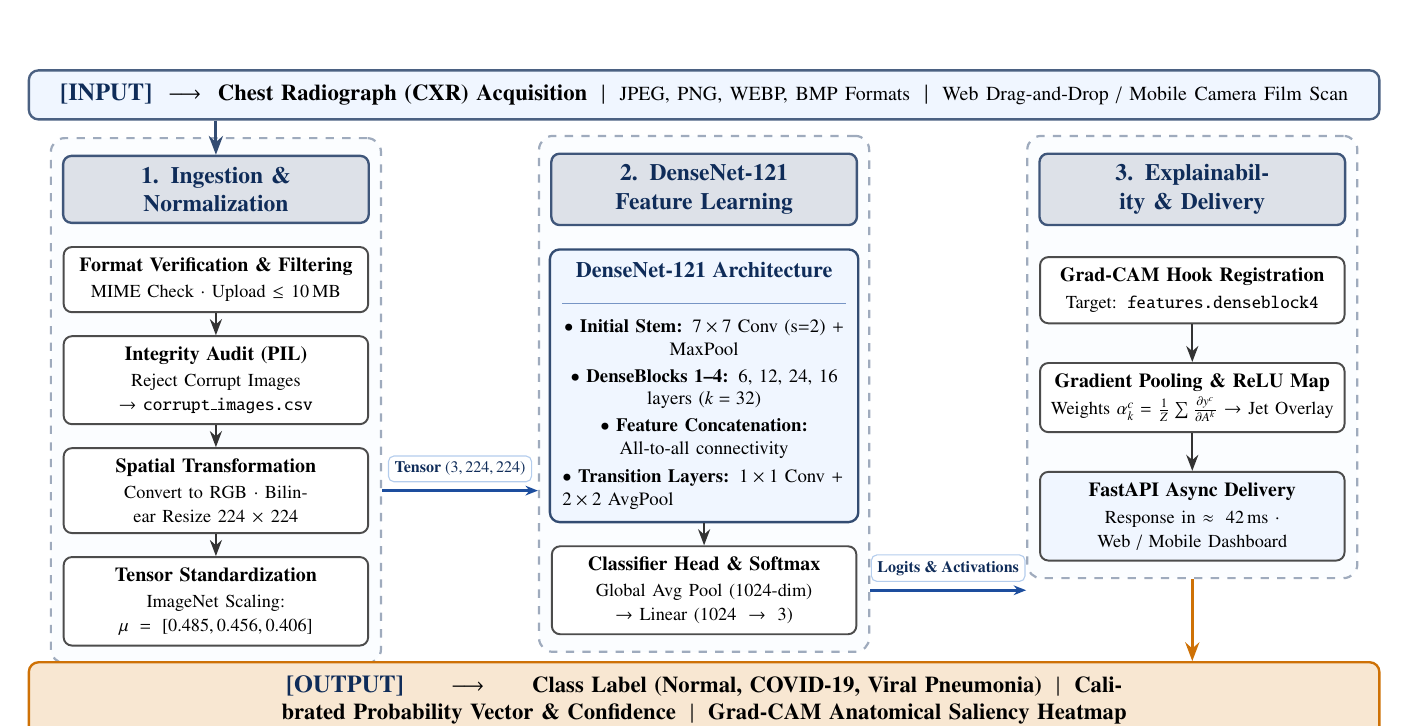
\begin{tikzpicture}[
    x=1cm, y=1cm,
    font=\sffamily,
    inout/.style={
        rectangle, rounded corners=3.5pt, line width=0.85pt,
        inner sep=5pt, align=center,
        font=\fontsize{8.2}{9.8}\selectfont
    },
    hdrbox/.style={
        rectangle, draw=lavenderDark!80, line width=0.85pt, fill=lavenderDark!14,
        rounded corners=3pt, inner sep=4pt, align=center,
        text width=3.60cm,
        font=\fontsize{8.5}{10.2}\selectfont\bfseries\color{lavenderDark}
    },
    stepbox/.style={
        rectangle, draw=black!70, line width=0.7pt, fill=white,
        rounded corners=3pt, inner sep=3.8pt, align=center,
        text width=3.60cm,
        font=\fontsize{7.2}{8.5}\selectfont
    },
    enginebox/.style={
        rectangle, draw=lavenderDark!85, line width=0.85pt, fill=lavenderLight,
        rounded corners=3.5pt, inner sep=4.5pt, align=left,
        text width=3.60cm,
        font=\fontsize{7.0}{8.5}\selectfont
    },
    stagebox/.style={
        rectangle, draw=lavenderDark!40, dashed, rounded corners=5pt, line width=0.8pt,
        fill=lavenderLight!25, inner xsep=4pt, inner ysep=6pt
    },
    flowarr/.style={
        -{Stealth[scale=0.85]}, line width=0.85pt, draw=black!80
    },
    transarr/.style={
        -{Stealth[length=4.5pt, width=3.5pt]}, line width=1.1pt, draw=lavenderMedium
    }
]

    % 1. TOP: INPUT BAR
    \node [inout, fill=lavenderLight, draw=lavenderDark!75, text width=16.8cm] (input_node) at (0, 3.40) {
        \textbf{\fontsize{8.8}{10.4}\selectfont\color{lavenderDark}[INPUT]} $\;\longrightarrow\;$
        \textbf{Chest Radiograph (CXR) Acquisition}\; $\vert$\;
        {\fontsize{7.2}{8.5}\selectfont JPEG, PNG, WEBP, BMP Formats}\; $\vert$\;
        {\fontsize{7.2}{8.5}\selectfont Web Drag-and-Drop / Mobile Camera Film Scan}
    };

    % 2. MIDDLE: 3-STAGE HORIZONTAL PIPELINE

    % --- STAGE 1: INGESTION & PREPROCESSING ---
    \node [hdrbox] (h1) at (-6.20, 2.20) {1. Ingestion \& Normalization};
    \node [stepbox, below=0.28cm of h1] (s1_1) {
        \textbf{Format Verification \& Filtering}\\[0.15em]
        {\fontsize{6.6}{7.8}\selectfont MIME Check $\cdot$ Upload $\le 10$\,MB}
    };
    \node [stepbox, below=0.28cm of s1_1] (s1_2) {
        \textbf{Integrity Audit (PIL)}\\[0.15em]
        {\fontsize{6.6}{7.8}\selectfont Reject Corrupt Images $\to$ \texttt{corrupt\_images.csv}}
    };
    \node [stepbox, below=0.28cm of s1_2] (s1_3) {
        \textbf{Spatial Transformation}\\[0.15em]
        {\fontsize{6.6}{7.8}\selectfont Convert to RGB $\cdot$ Bilinear Resize $224\times 224$}
    };
    \node [stepbox, below=0.28cm of s1_3] (s1_4) {
        \textbf{Tensor Standardization}\\[0.15em]
        {\fontsize{6.6}{7.8}\selectfont ImageNet Scaling: $\mu=[0.485,0.456,0.406]$}
    };

    \draw [flowarr] (s1_1) -- (s1_2);
    \draw [flowarr] (s1_2) -- (s1_3);
    \draw [flowarr] (s1_3) -- (s1_4);

    \begin{scope}[on background layer]
    \node [stagebox, fit=(h1) (s1_4)] (stage1) {};
    \end{scope}

    % --- STAGE 2: DENSENET-121 INFERENCE ---
    \node [hdrbox] (h2) at (0, 2.20) {2. DenseNet-121 Feature Learning};
    \node [enginebox, below=0.28cm of h2] (s2_1) {
        \centering\textbf{\fontsize{8.0}{9.5}\selectfont\color{lavenderDark}DenseNet-121 Architecture}\\[0.2em]
        {\color{lavenderMedium!60}\rule{\linewidth}{0.5pt}}\\[0.28em]
        {\fontsize{6.8}{8.2}\selectfont
        $\bullet$ \textbf{Initial Stem:} $7\times 7$ Conv (s=2) + MaxPool\\[0.22em]
        $\bullet$ \textbf{DenseBlocks 1--4:} 6, 12, 24, 16 layers ($k=32$)\\[0.22em]
        $\bullet$ \textbf{Feature Concatenation:} All-to-all connectivity\\[0.22em]
        $\bullet$ \textbf{Transition Layers:} $1\times 1$ Conv + $2\times 2$ AvgPool}
    };

    \node [stepbox, below=0.28cm of s2_1] (s2_2) {
        \textbf{Classifier Head \& Softmax}\\[0.15em]
        {\fontsize{6.6}{7.8}\selectfont Global Avg Pool ($1024$-dim) $\to$ Linear ($1024\to 3$)}
    };

    \draw [flowarr] (s2_1) -- (s2_2);

    \begin{scope}[on background layer]
    \node [stagebox, fit=(h2) (s2_2)] (stage2) {};
    \end{scope}

    % --- STAGE 3: GRAD-CAM & DELIVERY ---
    \node [hdrbox] (h3) at (6.20, 2.20) {3. Explainability \& Delivery};
    \node [stepbox, below=0.38cm of h3] (s3_1) {
        \textbf{Grad-CAM Hook Registration}\\[0.2em]
        {\fontsize{6.6}{7.8}\selectfont Target: \texttt{features.denseblock4}}
    };
    \node [stepbox, below=0.48cm of s3_1] (s3_2) {
        \textbf{Gradient Pooling \& ReLU Map}\\[0.2em]
        {\fontsize{6.6}{7.8}\selectfont Weights $\alpha_k^c = \frac{1}{Z}\sum \frac{\partial y^c}{\partial A^k} \to$ Jet Overlay}
    };
    \node [stepbox, below=0.48cm of s3_2, fill=lavenderLight] (s3_3) {
        \textbf{FastAPI Async Delivery}\\[0.2em]
        {\fontsize{6.6}{7.8}\selectfont Response in $\approx 42$\,ms $\cdot$ Web / Mobile Dashboard}
    };

    \draw [flowarr] (s3_1) -- (s3_2);
    \draw [flowarr] (s3_2) -- (s3_3);

    \begin{scope}[on background layer]
    \node [stagebox, fit=(h3) (s3_3)] (stage3) {};
    \end{scope}

    % Transition arrows between stages with non-overlapping white badges
    \draw [transarr] (stage1.east |- s1_3) -- 
        node[above=3pt, fill=white, draw=lavenderBorder, line width=0.4pt, rounded corners=2pt, inner sep=2.2pt, font=\fontsize{5.8}{6.8}\selectfont\bfseries\color{lavenderDark}]{Tensor $(3, 224, 224)$} (stage2.west |- s1_3);

    \draw [transarr] (stage2.east |- s2_2) -- 
        node[above=3pt, fill=white, draw=lavenderBorder, line width=0.4pt, rounded corners=2pt, inner sep=2.2pt, font=\fontsize{5.8}{6.8}\selectfont\bfseries\color{lavenderDark}]{Logits \& Activations} (stage3.west |- s2_2);

    \draw [flowarr, line width=1.1pt, draw=lavenderDark!85] (input_node.south -| h1.north) -- (h1.north);

    % 3. BOTTOM: OUTPUT BAR
    \node [inout, fill=prismGold!18, draw=prismGold!95!black, text width=16.8cm, below=0.50cm of $(stage1.south)!0.5!(stage3.south)$] (output_node) {
        \textbf{\fontsize{8.8}{10.4}\selectfont\color{lavenderDark}[OUTPUT]} $\;\longrightarrow\;$
        \textbf{Class Label (Normal, COVID-19, Viral Pneumonia)}\; $\vert$\;
        \textbf{Calibrated Probability Vector \& Confidence}\; $\vert$\;
        \textbf{Grad-CAM Anatomical Saliency Heatmap}
    };

    \draw [flowarr, line width=1.1pt, draw=prismGold!95!black] (stage3.south -| h3.south) -- (output_node.north -| h3.south);

\end{tikzpicture}
\end{document}
}
    \caption{Overall end-to-end system flow architecture from raw radiograph ingestion to clinical report generation.}
    \label{fig:system_flow}
\end{figure}

\section{System Flowchart and Algorithms}

\subsection{System Flowchart}
Figure~\ref{fig:multiagent_flowchart} maps the decision pathways and exception branches executing during an inference request.

\begin{figure}[H]
    \centering
    \adjustbox{max width=0.98\linewidth, max height=0.72\textheight, keepaspectratio, center}{\documentclass[tikz,border=10pt]{standalone}
\usepackage{tikz}
\usepackage{fontawesome5}
\usepackage{amsmath,amssymb}
\usetikzlibrary{arrows.meta,positioning,fit,backgrounds,calc,shadows,shapes.geometric}

% Color definitions
\definecolor{lavenderDark}{RGB}{15, 44, 89}
\definecolor{lavenderDeep}{RGB}{10, 28, 58}
\definecolor{lavenderMedium}{RGB}{29, 78, 158}
\definecolor{lavenderLight}{RGB}{240, 246, 255}
\definecolor{lavenderBorder}{RGB}{180, 205, 237}
\definecolor{prismNavy}{RGB}{15, 44, 89}
\definecolor{prismBlue}{RGB}{29, 78, 158}
\definecolor{prismTeal}{RGB}{13, 148, 136}
\definecolor{prismGold}{RGB}{217, 119, 6}
\definecolor{prismDark}{RGB}{15, 23, 42}
\definecolor{statusFail}{RGB}{220, 38, 38}
\definecolor{cInput}{RGB}{241, 245, 249}
\definecolor{cStem}{RGB}{224, 242, 254}
\definecolor{cStage1}{RGB}{209, 250, 229}
\definecolor{cStage2}{RGB}{254, 243, 199}
\definecolor{cHead}{RGB}{219, 234, 254}

\begin{document}
% Complete Flowchart for Deep Learning Early Lung Disease Detection
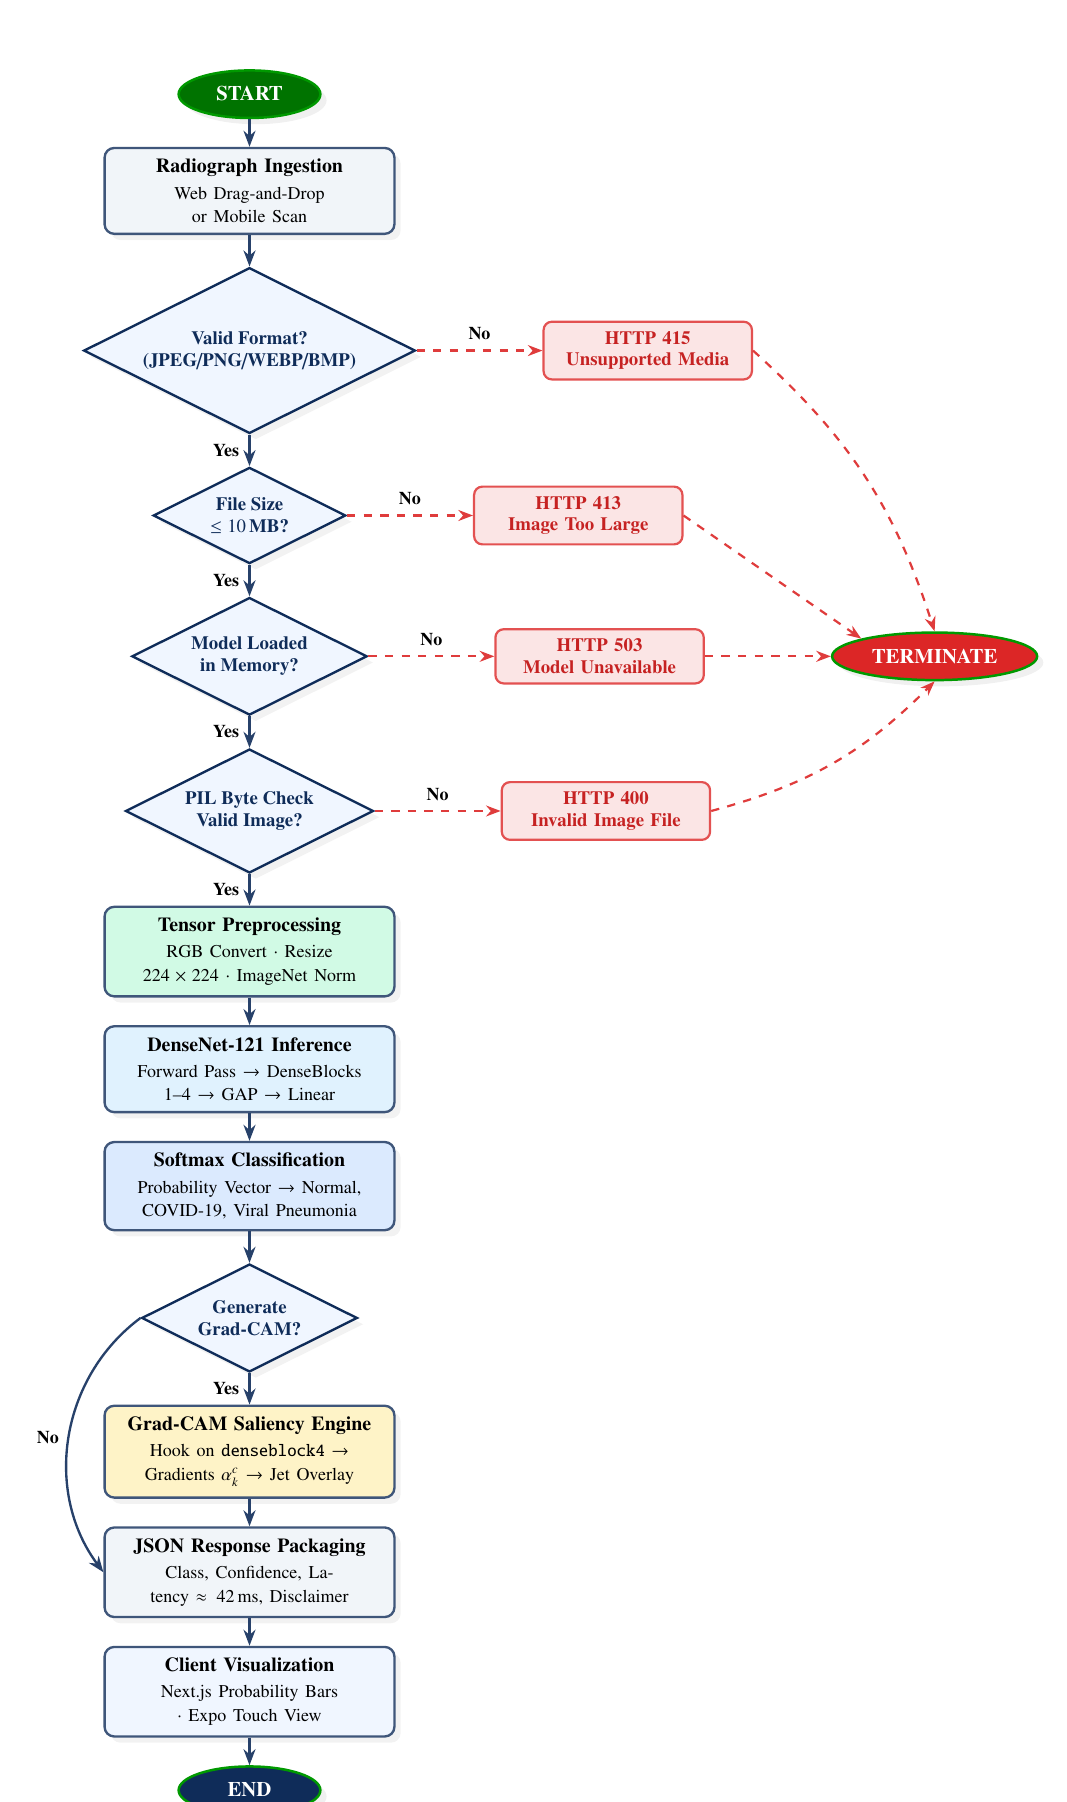
\begin{tikzpicture}[
  x=1cm, y=1cm,
  font=\sffamily,
  startend/.style={
    ellipse, draw=green!60!black, fill=green!45!black, text=white,
    line width=0.9pt, inner sep=3.5pt, font=\fontsize{7.5}{8.5}\selectfont\bfseries,
    minimum width=1.80cm, minimum height=0.60cm, drop shadow={opacity=0.12}
  },
  procbox/.style={
    rectangle, rounded corners=3.5pt,
    draw=lavenderDark!80, fill=white, text=black,
    line width=0.85pt, inner sep=4.0pt, font=\fontsize{7.2}{8.5}\selectfont,
    minimum height=0.75cm, text width=3.40cm, align=center, drop shadow={opacity=0.10}
  },
  decision/.style={
    diamond, aspect=2.0,
    draw=prismNavy, fill=lavenderLight, text=prismNavy,
    line width=0.85pt, inner sep=2.5pt, font=\fontsize{6.8}{8.0}\selectfont\bfseries,
    align=center, drop shadow={opacity=0.10}
  },
  errorbox/.style={
    rectangle, rounded corners=3pt,
    draw=statusFail!80, fill=statusFail!12, text=statusFail!90!black,
    line width=0.80pt, inner sep=3.5pt, font=\fontsize{6.8}{7.8}\selectfont\bfseries,
    minimum height=0.65cm, text width=2.40cm, align=center
  },
  flowarr/.style={
    -{Stealth[scale=0.85]}, line width=0.85pt, draw=lavenderDark!90
  },
  failarr/.style={
    -{Stealth[scale=0.80]}, line width=0.80pt, draw=statusFail!90, dashed
  }
]

  % Central Column - Main Processing Flow
  \node[startend] (start) at (0, 11.20) {START};

  \node[procbox, fill=cInput, below=0.35cm of start] (upload) {%
    \textbf{Radiograph Ingestion}\\[1pt]
    {\fontsize{6.5}{7.5}\selectfont Web Drag-and-Drop or Mobile Scan}%
  };

  \node[decision, below=0.40cm of upload] (d_mime) {%
    Valid Format?\\(JPEG/PNG/WEBP/BMP)%
  };

  \node[decision, below=0.40cm of d_mime] (d_size) {%
    File Size\\$\le 10$\,MB?%
  };

  \node[decision, below=0.40cm of d_size] (d_model) {%
    Model Loaded\\in Memory?%
  };

  \node[decision, below=0.40cm of d_model] (d_pil) {%
    PIL Byte Check\\Valid Image?%
  };

  \node[procbox, fill=cStage1, below=0.40cm of d_pil] (preprocess) {%
    \textbf{Tensor Preprocessing}\\[1pt]
    {\fontsize{6.5}{7.5}\selectfont RGB Convert $\cdot$ Resize $224\times 224$ $\cdot$ ImageNet Norm}%
  };

  \node[procbox, fill=cStem, below=0.35cm of preprocess] (infer) {%
    \textbf{DenseNet-121 Inference}\\[1pt]
    {\fontsize{6.5}{7.5}\selectfont Forward Pass $\to$ DenseBlocks 1--4 $\to$ GAP $\to$ Linear}%
  };

  \node[procbox, fill=cHead, below=0.35cm of infer] (softmax) {%
    \textbf{Softmax Classification}\\[1pt]
    {\fontsize{6.5}{7.5}\selectfont Probability Vector $\to$ Normal, COVID-19, Viral Pneumonia}%
  };

  \node[decision, below=0.40cm of softmax] (d_gradcam) {%
    Generate\\Grad-CAM?%
  };

  \node[procbox, fill=cStage2, below=0.40cm of d_gradcam] (gradcam) {%
    \textbf{Grad-CAM Saliency Engine}\\[1pt]
    {\fontsize{6.5}{7.5}\selectfont Hook on \texttt{denseblock4} $\to$ Gradients $\alpha_k^c$ $\to$ Jet Overlay}%
  };

  \node[procbox, fill=cInput, below=0.35cm of gradcam] (respond) {%
    \textbf{JSON Response Packaging}\\[1pt]
    {\fontsize{6.5}{7.5}\selectfont Class, Confidence, Latency $\approx 42$\,ms, Disclaimer}%
  };

  \node[procbox, fill=lavenderLight, below=0.35cm of respond] (render) {%
    \textbf{Client Visualization}\\[1pt]
    {\fontsize{6.5}{7.5}\selectfont Next.js Probability Bars $\cdot$ Expo Touch View}%
  };

  \node[startend, fill=lavenderDark, below=0.35cm of render] (end) {END};

  % Error Column (Right Side)
  \node[errorbox, right=1.60cm of d_mime] (e_mime) {HTTP 415\\Unsupported Media};
  \node[errorbox, right=1.60cm of d_size] (e_size) {HTTP 413\\Image Too Large};
  \node[errorbox, right=1.60cm of d_model] (e_model) {HTTP 503\\Model Unavailable};
  \node[errorbox, right=1.60cm of d_pil] (e_pil) {HTTP 400\\Invalid Image File};

  % Downward Connections
  \draw[flowarr] (start) -- (upload);
  \draw[flowarr] (upload) -- (d_mime);
  \draw[flowarr] (d_mime) -- node[left, font=\fontsize{6.5}{7.5}\selectfont\bfseries]{Yes} (d_size);
  \draw[flowarr] (d_size) -- node[left, font=\fontsize{6.5}{7.5}\selectfont\bfseries]{Yes} (d_model);
  \draw[flowarr] (d_model) -- node[left, font=\fontsize{6.5}{7.5}\selectfont\bfseries]{Yes} (d_pil);
  \draw[flowarr] (d_pil) -- node[left, font=\fontsize{6.5}{7.5}\selectfont\bfseries]{Yes} (preprocess);
  \draw[flowarr] (preprocess) -- (infer);
  \draw[flowarr] (infer) -- (softmax);
  \draw[flowarr] (softmax) -- (d_gradcam);
  \draw[flowarr] (d_gradcam) -- node[left, font=\fontsize{6.5}{7.5}\selectfont\bfseries]{Yes} (gradcam);
  \draw[flowarr] (gradcam) -- (respond);
  \draw[flowarr] (respond) -- (render);
  \draw[flowarr] (render) -- (end);

  % Branch around Grad-CAM when No
  \draw[flowarr] (d_gradcam.west) to[bend right=45] node[left, font=\fontsize{6.5}{7.5}\selectfont\bfseries]{No} (respond.west);

  % Error Branches
  \draw[failarr] (d_mime) -- node[above, font=\fontsize{6.5}{7.5}\selectfont\bfseries]{No} (e_mime);
  \draw[failarr] (d_size) -- node[above, font=\fontsize{6.5}{7.5}\selectfont\bfseries]{No} (e_size);
  \draw[failarr] (d_model) -- node[above, font=\fontsize{6.5}{7.5}\selectfont\bfseries]{No} (e_model);
  \draw[failarr] (d_pil) -- node[above, font=\fontsize{6.5}{7.5}\selectfont\bfseries]{No} (e_pil);

  % Terminate Error paths to common error end
  \node[startend, fill=statusFail, right=1.60cm of e_model] (err_end) {TERMINATE};
  \draw[failarr] (e_mime.east) to[bend left=15] (err_end.north);
  \draw[failarr] (e_size.east) -- (err_end.north west);
  \draw[failarr] (e_model.east) -- (err_end.west);
  \draw[failarr] (e_pil.east) to[bend right=15] (err_end.south);

\end{tikzpicture}
\end{document}
}
    \caption{System flowchart detailing radiograph ingestion, validation stages, DenseNet-121 inference, Grad-CAM generation, and clinical reporting.}
    \label{fig:multiagent_flowchart}
\end{figure}

\subsection{System Algorithm}
The complete operational algorithm governing model training, evaluation, inference, and explainability is formalized below across twelve sequential operational steps:

\subsubsection*{Step 1: Radiograph Acquisition and File Stream Sanitization}
\begin{enumerate}
  \item[\textbf{1.1}] Ingest raw radiograph file payload $\mathcal{F}_{\text{in}}$ via HTTP multipart form upload or local dataset scanner.
  \item[\textbf{1.2}] Perform MIME header verification against authorized types: $\mathrm{MIME} \in \{\texttt{image/jpeg}, \texttt{image/png}, \texttt{image/webp}, \texttt{image/bmp}\}$.
  \item[\textbf{1.3}] Enforce payload boundary limit: Verify $\mathrm{size}(\mathcal{F}_{\text{in}}) \le 10\,\mathrm{MB}$; return HTTP 413 on violation.
  \item[\textbf{1.4}] Execute byte-level verification using Python Imaging Library (PIL):
    \begin{equation}
      \mathrm{Status} = \mathrm{VerifyImageBytes}(\mathcal{F}_{\text{in}})
    \end{equation}
    Record corrupt file paths in \texttt{corrupt\_images.csv} and reject unreadable inputs with HTTP 400.
\end{enumerate}

\subsubsection*{Step 2: Stratified Partitioning and Class-Balancing Pipeline}
\begin{enumerate}
  \item[\textbf{2.1}] Discover dataset classes $\mathcal{C} = \{\text{Normal}, \text{COVID}, \text{Viral Pneumonia}\}$ from subfolder structure.
  \item[\textbf{2.2}] Partition verified samples into stratified splits with fixed random seed $s = 42$:
    \begin{equation}
      \mathcal{D}_{\text{train}} : \mathcal{D}_{\text{val}} : \mathcal{D}_{\text{test}} = 0.70 : 0.15 : 0.15
    \end{equation}
  \item[\textbf{2.3}] Enforce identical class proportions across all three splits to prevent distributional shift.
\end{enumerate}

\subsubsection*{Step 3: Spatial Standardization and Stochastic Data Augmentation}
\begin{enumerate}
  \item[\textbf{3.1}] Convert valid single-channel grayscale or 4-channel RGBA images to standard 3-channel RGB:
    \begin{equation}
      \mathbf{I}_{\text{rgb}} = \mathrm{ConvertRGB}(\mathbf{I}) \in \mathbb{R}^{H \times W \times 3}
    \end{equation}
  \item[\textbf{3.2}] Apply bilinear interpolation to standardize spatial resolution: $\mathbf{I}_{\text{res}} = \mathrm{Resize}(\mathbf{I}_{\text{rgb}}, (224, 224))$.
  \item[\textbf{3.3}] Apply stochastic augmentation operators during training:
    \begin{itemize}
      \item[\textbf{3.3.1}] Random Horizontal Flip with probability $p = 0.50$.
      \item[\textbf{3.3.2}] Random Rotation within bounds $\theta \in [-7^\circ, +7^\circ]$.
      \item[\textbf{3.3.3}] Photometric Color Jitter with brightness and contrast factors $\delta = 0.08$.
    \end{itemize}
\end{enumerate}

\subsubsection*{Step 4: Tensor Standardization and Normalization}
\begin{enumerate}
  \item[\textbf{4.1}] Convert augmented image matrix into Float32 tensor scaled to $[0.0, 1.0]$.
  \item[\textbf{4.2}] Standardize channels using standard ImageNet mean $\boldsymbol{\mu}$ and standard deviation $\boldsymbol{\sigma}$:
    \begin{equation}
      \mathbf{x}_{c, i, j} = \frac{\mathbf{I}_{c, i, j} - \mu_c}{\sigma_c} \quad \text{for } c \in \{R, G, B\}
    \end{equation}
    where $\boldsymbol{\mu} = [0.485, 0.456, 0.406]$ and $\boldsymbol{\sigma} = [0.229, 0.224, 0.225]$.
  \item[\textbf{4.3}] Pin memory and allocate tensor to active computing device (CUDA GPU or CPU).
\end{enumerate}

\subsubsection*{Step 5: DenseNet-121 Feature Learning and Connectivity Formulation}
\begin{enumerate}
  \item[\textbf{5.1}] Pass input tensor $\mathbf{x} \in \mathbb{R}^{3 \times 224 \times 224}$ through the initial convolutional stem:
    \begin{equation}
      \mathbf{x}_0 = \mathrm{MaxPool}_{3\times 3, s=2}\Big(\mathrm{Conv}_{7\times 7, s=2}(\mathbf{x})\Big) \in \mathbb{R}^{64 \times 56 \times 56}
    \end{equation}
  \item[\textbf{5.2}] Propagate through four DenseBlocks, where layer $l$ receives feature maps from all prior layers:
    \begin{equation}
      \mathbf{x}_l = H_l\big([\mathbf{x}_0, \mathbf{x}_1, \dots, \mathbf{x}_{l-1}]\big)
    \end{equation}
  \item[\textbf{5.3}] Enforce composite transformation $H_l$: $\mathrm{BN} \to \mathrm{ReLU} \to \mathrm{Conv}_{1\times 1} (4k) \to \mathrm{BN} \to \mathrm{ReLU} \to \mathrm{Conv}_{3\times 3} (k)$ with growth rate $k=32$.
\end{enumerate}

\subsubsection*{Step 6: Transition Downsampling and Feature Dimension Compression}
\begin{enumerate}
  \item[\textbf{6.1}] Connect consecutive DenseBlocks using Transition Layers to reduce spatial dimensions:
    \begin{equation}
      \mathbf{x}_{\text{trans}} = \mathrm{AvgPool}_{2\times 2, s=2}\Big(\mathrm{Conv}_{1\times 1}\big(\mathbf{x}_{\text{dense}}\big)\Big)
    \end{equation}
  \item[\textbf{6.2}] Apply channel compression factor $\theta = 0.50$ in the $1\times 1$ convolution to constrain feature map inflation.
\end{enumerate}

\subsubsection*{Step 7: Global Average Pooling and Latent Embedding Extraction}
\begin{enumerate}
  \item[\textbf{7.1}] Extract the terminal feature map from \texttt{denseblock4} of dimension $1024 \times 7 \times 7$.
  \item[\textbf{7.2}] Collapse spatial dimensions via Global Average Pooling (GAP) to obtain a compact latent vector:
    \begin{equation}
      \mathbf{h} = \frac{1}{7 \times 7} \sum_{i=1}^7 \sum_{j=1}^7 \mathbf{A}_{i, j} \in \mathbb{R}^{1024}
    \end{equation}
\end{enumerate}

\subsubsection*{Step 8: Multi-Class Linear Classification and Softmax Logit Scoring}
\begin{enumerate}
  \item[\textbf{8.1}] Project the 1024-dimensional representation through the linear classification head:
    \begin{equation}
      \mathbf{z} = \mathbf{W}_{\text{cls}} \mathbf{h} + \mathbf{b}_{\text{cls}} \in \mathbb{R}^3
    \end{equation}
  \item[\textbf{8.2}] Compute normalized posterior class probabilities via Softmax:
    \begin{equation}
      \hat{y}_c = \frac{\exp(z_c)}{\sum_{j=1}^3 \exp(z_j)} \quad \text{for } c \in \{\text{Normal}, \text{COVID}, \text{Viral Pneumonia}\}
    \end{equation}
  \item[\textbf{8.3}] Select predicted disease class $\hat{c} = \arg\max_c \hat{y}_c$ and confidence $\kappa = \max_c \hat{y}_c$.
\end{enumerate}

\subsubsection*{Step 9: Optimization, Decoupled Weight Decay, and Early Stopping}
\begin{enumerate}
  \item[\textbf{9.1}] Update network parameters $\theta$ using the AdamW optimizer with initial learning rate $\eta = 10^{-4}$ and weight decay $\lambda = 10^{-4}$.
  \item[\textbf{9.2}] Track validation loss $\mathcal{L}_{\text{val}}$ after each training epoch:
    \begin{equation}
      \mathcal{L}_{\text{val}} = -\frac{1}{|\mathcal{D}_{\text{val}}|} \sum_{i \in \mathcal{D}_{\text{val}}} \log \hat{y}_{i, y_i}
    \end{equation}
  \item[\textbf{9.3}] If $\mathcal{L}_{\text{val}}$ achieves a new global minimum, save model checkpoint to \texttt{checkpoints/best\_model.pt}.
  \item[\textbf{9.4}] If $\mathcal{L}_{\text{val}}$ fails to improve for $p = 6$ consecutive epochs, trigger early stopping to halt training.
\end{enumerate}

\subsubsection*{Step 10: Grad-CAM Explainability Hook and Gradient Pooling}
\begin{enumerate}
  \item[\textbf{10.1}] Register forward and full-backward hooks on the final convolutional layer: \texttt{model.features.denseblock4}.
  \item[\textbf{10.2}] Perform a backward pass with respect to predicted class logit $z_{\hat{c}}$:
    \begin{equation}
      \mathbf{g}^k = \frac{\partial z_{\hat{c}}}{\partial A^k}
    \end{equation}
  \item[\textbf{10.3}] Compute neuron importance weight $\alpha_k^{\hat{c}}$ by global average pooling gradients across spatial coordinates $U \times V$:
    \begin{equation}
      \alpha_k^{\hat{c}} = \frac{1}{U \times V} \sum_{i=1}^U \sum_{j=1}^V g_{i, j}^k
    \end{equation}
  \item[\textbf{10.4}] Generate the rectified class activation map:
    \begin{equation}
      M_{\text{cam}} = \mathrm{ReLU}\left( \sum_{k=1}^{1024} \alpha_k^{\hat{c}} A^k \right)
    \end{equation}
\end{enumerate}

\subsubsection*{Step 11: Spatial Upsampling, Jet Colormap Synthesis, and Visual Superimposition}
\begin{enumerate}
  \item[\textbf{11.1}] Normalize activation map to range $[0.0, 1.0]$: $M_{\text{norm}} = \frac{M_{\text{cam}}}{\max(M_{\text{cam}}) + 10^{-8}}$.
  \item[\textbf{11.2}] Upsample $M_{\text{norm}}$ from $7 \times 7$ to input resolution $224 \times 224$ via bilinear interpolation.
  \item[\textbf{11.3}] Map scalar intensities to the RGB Jet colormap and alpha-blend with original radiograph:
    \begin{equation}
      \mathbf{I}_{\text{overlay}} = \beta \cdot \mathbf{I}_{\text{orig}} + (1 - \beta) \cdot \mathrm{JetColor}\big(M_{\text{norm}}\big)
    \end{equation}
    where $\beta = 0.60$ controls transparency.
\end{enumerate}

\subsubsection*{Step 12: Asynchronous Production Serving, Multi-Platform Telemetry, and Safety Gating}
\begin{enumerate}
  \item[\textbf{12.1}] Package results into strongly-typed Pydantic response:
    \begin{equation}
    \begin{aligned}
      \mathcal{R} = \big\{ & \texttt{"success"}: \mathrm{true}, \; \texttt{"prediction"}: \hat{c}, \; \texttt{"confidence"}: \kappa, \\
                           & \texttt{"probabilities"}: \hat{\mathbf{y}}, \; \texttt{"latency\_ms"}: t \big\}
    \end{aligned}
    \end{equation}
  \item[\textbf{12.2}] Append mandatory clinical screening disclaimer: \textit{``Preliminary screening assistance only; this result is not a medical diagnosis.''}
  \item[\textbf{12.3}] Stream JSON payload to client; Next.js 15 renders probability bars and Expo mobile displays touch-zoomable overlay.
\end{enumerate}

\subsection{DenseNet-121 Structural Connectivity and Layer Decomposition}
Figure~\ref{fig:dag_scheduling_walkthrough} illustrates the structural decomposition and dense feedforward connectivity of DenseNet-121 alongside the Grad-CAM backward propagation path.

\begin{figure}[H]
    \centering
    \adjustbox{max width=0.98\linewidth, max height=0.68\textheight, keepaspectratio, center}{\documentclass[tikz,border=10pt]{standalone}
\usepackage{tikz}
\usepackage{fontawesome5}
\usepackage{amsmath,amssymb}
\usetikzlibrary{arrows.meta,positioning,fit,backgrounds,calc,shadows,shapes.geometric}

% Color definitions
\definecolor{lavenderDark}{RGB}{15, 44, 89}
\definecolor{lavenderDeep}{RGB}{10, 28, 58}
\definecolor{lavenderMedium}{RGB}{29, 78, 158}
\definecolor{lavenderLight}{RGB}{240, 246, 255}
\definecolor{lavenderBorder}{RGB}{180, 205, 237}
\definecolor{prismNavy}{RGB}{15, 44, 89}
\definecolor{prismBlue}{RGB}{29, 78, 158}
\definecolor{prismTeal}{RGB}{13, 148, 136}
\definecolor{prismGold}{RGB}{217, 119, 6}
\definecolor{prismDark}{RGB}{15, 23, 42}
\definecolor{prismSlate}{RGB}{100, 116, 139}
\definecolor{statusFail}{RGB}{220, 38, 38}
\definecolor{cInput}{RGB}{241, 245, 249}
\definecolor{cStem}{RGB}{224, 242, 254}
\definecolor{cStage1}{RGB}{209, 250, 229}
\definecolor{cStage2}{RGB}{254, 243, 199}
\definecolor{cStage3}{RGB}{254, 226, 226}
\definecolor{cStage4}{RGB}{207, 250, 254}
\definecolor{cHead}{RGB}{219, 234, 254}

\begin{document}
% DenseNet-121 Layer Decomposition and Dense Connectivity Graph
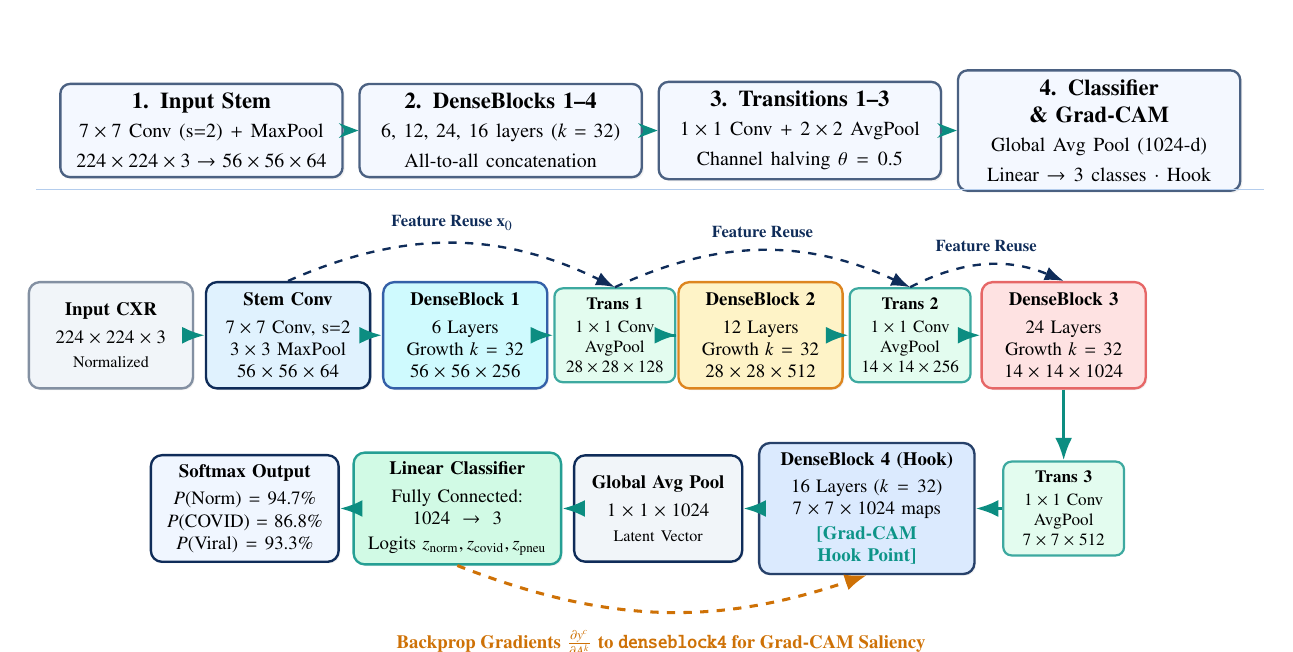
\begin{tikzpicture}[
  x=1cm, y=1cm,
  font=\sffamily,
  dagstep/.style={rectangle, rounded corners=3.5pt, minimum height=1.10cm,
    text width=3.35cm, align=center, draw=lavenderDark!75, fill=lavenderLight!75,
    line width=0.85pt, font=\fontsize{8.2}{9.8}\selectfont\bfseries,
    drop shadow={shadow xshift=0.8pt, shadow yshift=-0.8pt, opacity=0.10}},
  dagarrow/.style={-{Stealth[scale=0.85]}, line width=1.15pt, draw=prismTeal!95!black},
  blkbox/.style={rectangle, rounded corners=4pt, line width=0.85pt,
    minimum height=1.35cm, text width=1.85cm, align=center,
    font=\fontsize{6.8}{8.0}\selectfont, drop shadow={shadow xshift=0.6pt, shadow yshift=-0.6pt, opacity=0.12}},
  transbox/.style={rectangle, rounded corners=3pt, line width=0.80pt,
    draw=prismTeal!80, fill=cStage1!60, minimum height=1.15cm, text width=1.30cm, align=center,
    font=\fontsize{6.2}{7.3}\selectfont},
  skipconn/.style={-{Stealth[scale=0.75]}, line width=0.85pt, draw=prismNavy, dashed}
]

  % Row 1: 4-Stage Architectural Progression
  \node[dagstep] (s1) at (-5.70, 0) {1. Input Stem\\[2pt]\normalfont\fontsize{7.2}{8.5}\selectfont $7\times 7$ Conv (s=2) + MaxPool\\[1pt]$224\times 224\times 3 \to 56\times 56\times 64$};
  \node[dagstep] (s2) at (-1.90, 0) {2. DenseBlocks 1--4\\[2pt]\normalfont\fontsize{7.2}{8.5}\selectfont 6, 12, 24, 16 layers ($k=32$)\\[1pt]All-to-all concatenation};
  \node[dagstep] (s3) at (1.90, 0) {3. Transitions 1--3\\[2pt]\normalfont\fontsize{7.2}{8.5}\selectfont $1\times 1$ Conv + $2\times 2$ AvgPool\\[1pt]Channel halving $\theta=0.5$};
  \node[dagstep] (s4) at (5.70, 0) {4. Classifier \& Grad-CAM\\[2pt]\normalfont\fontsize{7.2}{8.5}\selectfont Global Avg Pool ($1024$-d)\\[1pt]Linear $\to 3$ classes $\cdot$ Hook};

  \draw[dagarrow] (s1) -- (s2);
  \draw[dagarrow] (s2) -- (s3);
  \draw[dagarrow] (s3) -- (s4);

  % Separator
  \draw[draw=lavenderBorder, line width=0.6pt] (-7.8, -0.75) -- (7.8, -0.75);

  % Row 2: Detailed Layer Decomposition Flow (Left-to-Right)
  \node[blkbox, fill=cInput, draw=prismSlate!80] (input_node) at (-6.85, -2.60) {
    \textbf{Input CXR}\\[2pt]
    $224\times 224\times 3$\\[1pt]
    {\fontsize{5.8}{6.8}\selectfont Normalized}
  };

  \node[blkbox, fill=cStem, draw=lavenderDark] (stem_node) at (-4.60, -2.60) {
    \textbf{Stem Conv}\\[2pt]
    $7\times 7$ Conv, s=2\\
    $3\times 3$ MaxPool\\
    $56\times 56\times 64$
  };

  \node[blkbox, fill=cStage4, draw=prismBlue!90] (db1) at (-2.35, -2.60) {
    \textbf{DenseBlock 1}\\[2pt]
    6 Layers\\
    Growth $k=32$\\
    $56\times 56\times 256$
  };

  \node[transbox] (tr1) at (-0.45, -2.60) {
    \textbf{Trans 1}\\[1pt]
    $1\times 1$ Conv\\
    AvgPool\\
    $28\times 28\times 128$
  };

  \node[blkbox, fill=cStage2, draw=prismGold!90] (db2) at (1.40, -2.60) {
    \textbf{DenseBlock 2}\\[2pt]
    12 Layers\\
    Growth $k=32$\\
    $28\times 28\times 512$
  };

  \node[transbox] (tr2) at (3.30, -2.60) {
    \textbf{Trans 2}\\[1pt]
    $1\times 1$ Conv\\
    AvgPool\\
    $14\times 14\times 256$
  };

  \node[blkbox, fill=cStage3, draw=statusFail!70] (db3) at (5.25, -2.60) {
    \textbf{DenseBlock 3}\\[2pt]
    24 Layers\\
    Growth $k=32$\\
    $14\times 14\times 1024$
  };

  % Row 3: Return Flow (Right-to-Left)
  \node[transbox] (tr3) at (5.25, -4.80) {
    \textbf{Trans 3}\\[1pt]
    $1\times 1$ Conv\\
    AvgPool\\
    $7\times 7\times 512$
  };

  \node[blkbox, fill=cHead, draw=lavenderDark!90, text width=2.50cm] (db4) at (2.75, -4.80) {
    \textbf{DenseBlock 4 (Hook)}\\[2pt]
    16 Layers ($k=32$)\\
    $7\times 7\times 1024$ maps\\[1pt]
    {\color{prismTeal}\textbf{[Grad-CAM Hook Point]}}
  };

  \node[blkbox, fill=cInput, draw=prismNavy, text width=1.90cm] (gap) at (0.10, -4.80) {
    \textbf{Global Avg Pool}\\[2pt]
    $1\times 1\times 1024$\\[1pt]
    {\fontsize{5.8}{6.8}\selectfont Latent Vector}
  };

  \node[blkbox, fill=cStage1, draw=prismTeal!90, text width=2.40cm] (head) at (-2.45, -4.80) {
    \textbf{Linear Classifier}\\[2pt]
    Fully Connected: $1024 \to 3$\\[1pt]
    Logits $z_{\text{norm}}, z_{\text{covid}}, z_{\text{pneu}}$
  };

  \node[blkbox, fill=lavenderLight, draw=lavenderDark, text width=2.15cm] (softmax) at (-5.15, -4.80) {
    \textbf{Softmax Output}\\[2pt]
    $P(\text{Norm}) = 94.7\%$\\
    $P(\text{COVID}) = 86.8\%$\\
    $P(\text{Viral}) = 93.3\%$
  };

  % Forward Flow Connections (explicit east to west for row 1, down for turn, east to west for row 2)
  \draw[->, >=Latex, line width=1.15pt, draw=prismTeal!95!black] (input_node.east) -- (stem_node.west);
  \draw[->, >=Latex, line width=1.15pt, draw=prismTeal!95!black] (stem_node.east) -- (db1.west);
  \draw[->, >=Latex, line width=1.15pt, draw=prismTeal!95!black] (db1.east) -- (tr1.west);
  \draw[->, >=Latex, line width=1.15pt, draw=prismTeal!95!black] (tr1.east) -- (db2.west);
  \draw[->, >=Latex, line width=1.15pt, draw=prismTeal!95!black] (db2.east) -- (tr2.west);
  \draw[->, >=Latex, line width=1.15pt, draw=prismTeal!95!black] (tr2.east) -- (db3.west);
  \draw[->, >=Latex, line width=1.15pt, draw=prismTeal!95!black] (db3.south) -- (tr3.north);
  \draw[->, >=Latex, line width=1.15pt, draw=prismTeal!95!black] (tr3.west) -- (db4.east);
  \draw[->, >=Latex, line width=1.15pt, draw=prismTeal!95!black] (db4.west) -- (gap.east);
  \draw[->, >=Latex, line width=1.15pt, draw=prismTeal!95!black] (gap.west) -- (head.east);
  \draw[->, >=Latex, line width=1.15pt, draw=prismTeal!95!black] (head.west) -- (softmax.east);

  % Dense Concatenation Skip Connections (curved lines representing intra-block feature reuse)
  \draw[->, >=Latex, line width=0.85pt, draw=prismNavy, dashed] (stem_node.north) to[bend left=25] node[above=1pt, font=\fontsize{6.0}{7.0}\selectfont\color{prismNavy}\bfseries]{Feature Reuse $\mathbf{x}_0$} (tr1.north);
  \draw[->, >=Latex, line width=0.85pt, draw=prismNavy, dashed] (tr1.north) to[bend left=25] node[above=1pt, font=\fontsize{6.0}{7.0}\selectfont\color{prismNavy}\bfseries]{Feature Reuse} (tr2.north);
  \draw[->, >=Latex, line width=0.85pt, draw=prismNavy, dashed] (tr2.north) to[bend left=25] node[above=1pt, font=\fontsize{6.0}{7.0}\selectfont\color{prismNavy}\bfseries]{Feature Reuse} (db3.north);

  % Backward Hook Arrow from Softmax / Head back to DenseBlock 4
  \draw[->, >=Latex, line width=1.1pt, draw=prismGold!95!black, dashed] 
    (head.south) to[bend right=20] 
    node[below=3pt, font=\fontsize{6.8}{8.0}\selectfont\bfseries\color{prismGold!95!black}]{Backprop Gradients $\frac{\partial y^c}{\partial A^k}$ to \texttt{denseblock4} for Grad-CAM Saliency} 
    (db4.south);

\end{tikzpicture}
\end{document}
}
    \caption{DenseNet-121 layer connectivity graph illustrating dense block feedforward concatenation, transition layer downsampling, and Grad-CAM backward propagation.}
    \label{fig:dag_scheduling_walkthrough}
\end{figure}

\section{Detailed Component Analysis}

\subsection{Data Storage, Model Artifacts, and Schema Connectors}
Figure~\ref{fig:db_schema} depicts the relational schema architecture connecting dataset partitions, training configurations, model checkpoints, evaluation metrics, and API payloads.

\begin{figure}[H]
    \centering
    \adjustbox{max width=0.98\linewidth, max height=0.72\textheight, keepaspectratio, center}{\documentclass[tikz,border=10pt]{standalone}
\usepackage{tikz}
\usepackage{fontawesome5}
\usepackage{amsmath,amssymb}
\usetikzlibrary{arrows.meta,positioning,fit,backgrounds,calc,shadows,shapes.geometric}

% Color definitions
\definecolor{lavenderDark}{RGB}{15, 44, 89}
\definecolor{lavenderDeep}{RGB}{10, 28, 58}
\definecolor{lavenderMedium}{RGB}{29, 78, 158}
\definecolor{lavenderLight}{RGB}{240, 246, 255}
\definecolor{lavenderBorder}{RGB}{180, 205, 237}
\definecolor{prismTeal}{RGB}{13, 148, 136}
\definecolor{prismMint}{RGB}{236, 253, 245}
\definecolor{prismGold}{RGB}{217, 119, 6}
\definecolor{prismDark}{RGB}{15, 23, 42}
\definecolor{cInput}{RGB}{241, 245, 249}
\definecolor{cPlanner}{RGB}{219, 234, 254}
\definecolor{cReact}{RGB}{209, 250, 229}
\definecolor{cTool}{RGB}{254, 243, 199}
\definecolor{cSafety}{RGB}{254, 226, 226}
\definecolor{cDeliverable}{RGB}{204, 251, 241}

\begin{document}
% Relational Entity & Storage Schema Connectors for Lung Disease Detection
\begin{tikzpicture}[
  x=1cm, y=1cm,
  font=\sffamily,
  tblcard/.style={
    rectangle, rounded corners=4pt, draw=lavenderDark!75, line width=0.85pt, fill=white,
    inner sep=5pt, text width=4.40cm, align=left,
    drop shadow={shadow xshift=1pt, shadow yshift=-1pt, opacity=0.12}
  },
  fkarrow/.style={
    -{Stealth[scale=0.85]}, line width=1.0pt, draw=lavenderDark!90
  },
  fklabel/.style={
    font=\fontsize{6.2}{7.2}\selectfont\bfseries, fill=white, inner sep=1.5pt, text=lavenderDark
  }
]

  % ================= COLUMN 1: DATASET & CONFIGURATION (x = -5.2) =================
  
  % Table 1: dataset_partition_schema
  \node[tblcard] (dataset) at (-5.2, 2.5) {%
    \centerline{\color{lavenderDark}\faFolderOpen\ \textbf{\fontsize{8.0}{9.5}\selectfont dataset\_partition\_store}}\\[3pt]
    \rule{\linewidth}{0.4pt}\\[3pt]
    {\fontsize{6.8}{8.0}\selectfont
    \textbf{\color{lavenderDark}[PK]} \texttt{image\_path}: \textit{string} (Indexed)\\
    \textbf{\color{prismTeal}[FLD]} \texttt{class\_label}: \textit{NORMAL/COVID/VIRAL}\\
    \textbf{\color{prismDark!80}[FLD]} \texttt{split}: \textit{train (70\%) / val / test}\\
    \textbf{\color{prismDark!80}[FLD]} \texttt{integrity}: \textit{valid / corrupt}\\
    \textbf{\color{prismDark!80}[FLD]} \texttt{tensor\_dims}: \textit{$(3, 224, 224)$ normalized}}
  };

  % Table 2: training_config_schema
  \node[tblcard, below=0.70cm of dataset] (config) {%
    \centerline{\color{lavenderDark}\faCogs\ \textbf{\fontsize{8.0}{9.5}\selectfont training\_config\_store}}\\[3pt]
    \rule{\linewidth}{0.4pt}\\[3pt]
    {\fontsize{6.8}{8.0}\selectfont
    \textbf{\color{lavenderDark}[PK]} \texttt{config\_id}: \textit{string} (UUID)\\
    \textbf{\color{prismDark!80}[FLD]} \texttt{image\_size}: \textit{224} $\cdot$ \texttt{batch\_size}: \textit{32}\\
    \textbf{\color{prismDark!80}[FLD]} \texttt{learning\_rate}: \textit{0.0001} (AdamW)\\
    \textbf{\color{prismDark!80}[FLD]} \texttt{weight\_decay}: \textit{0.0001}\\
    \textbf{\color{prismDark!80}[FLD]} \texttt{patience}: \textit{6 epochs} (EarlyStop)\\
    \textbf{\color{prismDark!80}[FLD]} \texttt{augmentations}: \textit{flip, rot $\pm 7^\circ$, jitter}}
  };

  % ================= COLUMN 2: MODEL CHECKPOINTS & EVALUATION (x = 0) =================
  
  % Table 3: model_checkpoint_schema
  \node[tblcard] (checkpoint) at (0, 2.5) {%
    \centerline{\color{lavenderDark}\faDatabase\ \textbf{\fontsize{8.0}{9.5}\selectfont model\_checkpoint\_store}}\\[3pt]
    \rule{\linewidth}{0.4pt}\\[3pt]
    {\fontsize{6.8}{8.0}\selectfont
    \textbf{\color{lavenderDark}[PK]} \texttt{checkpoint\_id}: \textit{timestamp}\\
    \textbf{\color{prismTeal}[FK]} \texttt{config\_id}: \textit{config reference}\\
    \textbf{\color{prismDark!80}[FLD]} \texttt{architecture}: \textit{DenseNet-121}\\
    \textbf{\color{prismDark!80}[FLD]} \texttt{lowest\_val\_loss}: \textit{0.1906 (ep 7)}\\
    \textbf{\color{prismDark!80}[FLD]} \texttt{weights\_path}: \textit{best\_model.pth}\\
    \textbf{\color{prismDark!80}[FLD]} \texttt{classes\_file}: \textit{classes.json}}
  };

  % Table 4: evaluation_telemetry_schema
  \node[tblcard, below=0.70cm of checkpoint] (eval) {%
    \centerline{\color{lavenderDark}\faChartLine\ \textbf{\fontsize{8.0}{9.5}\selectfont evaluation\_telemetry\_store}}\\[3pt]
    \rule{\linewidth}{0.4pt}\\[3pt]
    {\fontsize{6.8}{8.0}\selectfont
    \textbf{\color{lavenderDark}[PK]} \texttt{eval\_id}: \textit{UUID}\\
    \textbf{\color{prismTeal}[FK]} \texttt{checkpoint\_id}: \textit{model reference}\\
    \textbf{\color{prismDark!80}[FLD]} \texttt{test\_accuracy}: \textit{92.63\% (4546 imgs)}\\
    \textbf{\color{prismDark!80}[FLD]} \texttt{macro\_f1}: \textit{91.59\%} $\cdot$ \texttt{wt\_f1}: \textit{92.66\%}\\
    \textbf{\color{prismDark!80}[FLD]} \texttt{roc\_auc\_ovr}: \textit{98.50\%}\\
    \textbf{\color{prismDark!80}[FLD]} \texttt{class\_f1}: \textit{Norm: 94.7\%, Cov: 86.8\%}}
  };

  % ================= COLUMN 3: API CONTRACTS & CLIENT STATE (x = 5.2) =================
  
  % Table 5: api_prediction_schema
  \node[tblcard] (prediction) at (5.2, 2.5) {%
    \centerline{\color{lavenderDark}\faServer\ \textbf{\fontsize{8.0}{9.5}\selectfont api\_prediction\_schema}}\\[3pt]
    \rule{\linewidth}{0.4pt}\\[3pt]
    {\fontsize{6.8}{8.0}\selectfont
    \textbf{\color{lavenderDark}[PK]} \texttt{prediction\_id}: \textit{UUID}\\
    \textbf{\color{prismTeal}[FK]} \texttt{checkpoint\_id}: \textit{active model}\\
    \textbf{\color{prismDark!80}[FLD]} \texttt{success}: \textit{boolean (true)}\\
    \textbf{\color{prismDark!80}[FLD]} \texttt{predicted\_class}: \textit{string}\\
    \textbf{\color{prismDark!80}[FLD]} \texttt{confidence}: \textit{float (0.0 .. 1.0)}\\
    \textbf{\color{prismDark!80}[FLD]} \texttt{probabilities}: \textit{JSON map}\\
    \textbf{\color{prismDark!80}[FLD]} \texttt{processing\_time\_ms}: \textit{float ($\approx 42$\,ms)}\\
    \textbf{\color{prismDark!80}[FLD]} \texttt{safety\_message}: \textit{preliminary notice}}
  };

  % Table 6: client_ui_state_schema
  \node[tblcard, below=0.70cm of prediction] (client) {%
    \centerline{\color{lavenderDark}\faDesktop\ \textbf{\fontsize{8.0}{9.5}\selectfont client\_ui\_state\_schema}}\\[3pt]
    \rule{\linewidth}{0.4pt}\\[3pt]
    {\fontsize{6.8}{8.0}\selectfont
    \textbf{\color{lavenderDark}[PK]} \texttt{session\_id}: \textit{UUID}\\
    \textbf{\color{prismTeal}[FK]} \texttt{prediction\_id}: \textit{payload reference}\\
    \textbf{\color{prismDark!80}[FLD]} \texttt{image\_preview\_url}: \textit{blob/base64}\\
    \textbf{\color{prismDark!80}[FLD]} \texttt{gradcam\_overlay}: \textit{PNG heatmap}\\
    \textbf{\color{prismDark!80}[FLD]} \texttt{visual\_probabilities}: \textit{bar charts}\\
    \textbf{\color{prismDark!80}[FLD]} \texttt{client\_platform}: \textit{Web / Mobile Expo}}
  };

  % ================= RELATIONSHIPS / FOREIGN KEY CONNECTORS =================

  % 1. Config -> Checkpoint
  \draw[fkarrow] (config.east) to[bend right=20] 
    node[above=1pt, fklabel]{config\_id} (checkpoint.west);

  % 2. Dataset -> Checkpoint (Data used to train)
  \draw[fkarrow] (dataset.east) -- 
    node[above=1pt, fklabel]{train\_split} (checkpoint.west);

  % 3. Checkpoint -> Evaluation
  \draw[fkarrow] (checkpoint.south) -- 
    node[right=2pt, fklabel]{checkpoint\_id} (eval.north);

  % 4. Checkpoint -> API Prediction
  \draw[fkarrow] (checkpoint.east) -- 
    node[above=1pt, fklabel]{weights} (prediction.west);

  % 5. API Prediction -> Client UI State
  \draw[fkarrow] (prediction.south) -- 
    node[right=2pt, fklabel]{prediction\_id} (client.north);

  % 6. Eval metrics reference in Client UI
  \draw[fkarrow, dashed] (eval.east) -- 
    node[above=1pt, fklabel]{benchmarks} (client.west);

\end{tikzpicture}
\end{document}
}
    \caption{Relational entity and data storage schema connectors showing dataset partitions, model configurations, checkpoints, evaluation telemetry, and API contract specifications.}
    \label{fig:db_schema}
\end{figure}

\subsection{Level-1 Data Flow Architecture}
Figure~\ref{fig:data_flow_diagram} illustrates the Level-1 Data Flow Diagram (DFD), showing external entities, primary processing transformations, datastores, and telemetry feedback loops.

\begin{figure}[H]
    \centering
    \adjustbox{max width=0.98\linewidth, max height=0.72\textheight, keepaspectratio, center}{\documentclass[tikz,border=10pt]{standalone}
\usepackage{tikz}
\usepackage{amsmath,amssymb}
\usepackage{fontawesome5}
\usetikzlibrary{arrows.meta,positioning,fit,backgrounds,calc,shadows,shapes.geometric}

% Color definitions
\definecolor{lavenderDark}{RGB}{15, 44, 89}
\definecolor{lavenderDeep}{RGB}{10, 28, 58}
\definecolor{lavenderMedium}{RGB}{29, 78, 158}
\definecolor{lavenderLight}{RGB}{240, 246, 255}
\definecolor{lavenderBorder}{RGB}{180, 205, 237}
\definecolor{prismNavy}{RGB}{15, 44, 89}
\definecolor{prismBlue}{RGB}{29, 78, 158}
\definecolor{prismTeal}{RGB}{13, 148, 136}
\definecolor{prismGold}{RGB}{217, 119, 6}
\definecolor{prismDark}{RGB}{15, 23, 42}
\definecolor{cInput}{RGB}{241, 245, 249}
\definecolor{cStem}{RGB}{224, 242, 254}
\definecolor{cStage1}{RGB}{209, 250, 229}
\definecolor{cStage2}{RGB}{254, 243, 199}
\definecolor{cStage4}{RGB}{207, 250, 254}
\definecolor{cHead}{RGB}{219, 234, 254}

\begin{document}
% Level-1 Data Flow Diagram (DFD) for Lung Disease Detection
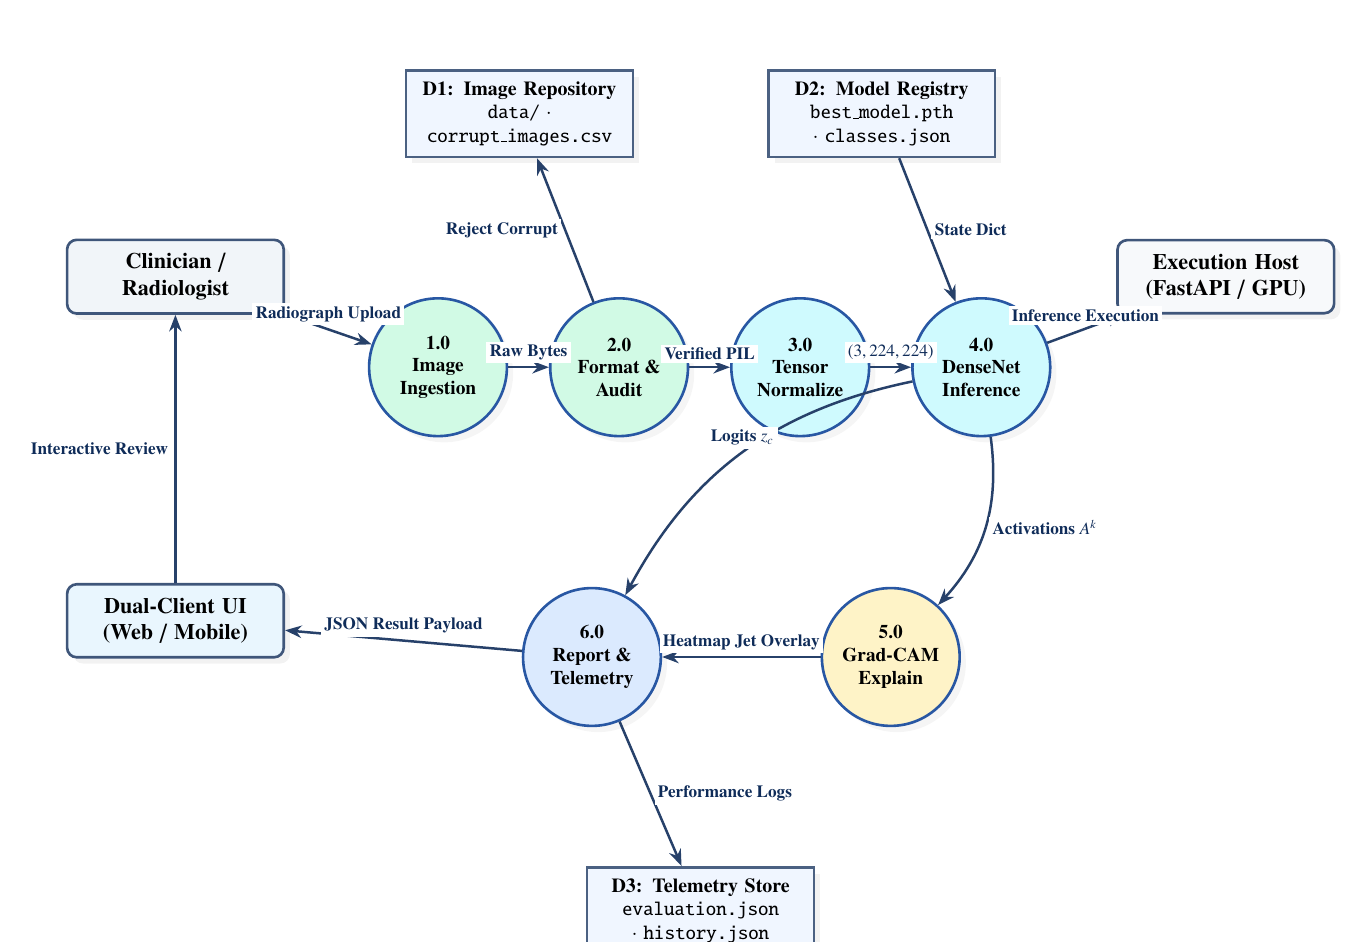
\begin{tikzpicture}[
  x=1.15cm, y=1.15cm,
  font=\sffamily,
  entity/.style={
    rectangle, draw=lavenderDark!80, line width=0.95pt, rounded corners=3.5pt,
    align=center, inner sep=5pt, font=\fontsize{8.0}{9.5}\selectfont\bfseries,
    text width=2.40cm, fill=cInput, drop shadow={opacity=0.10}
  },
  store/.style={
    rectangle, draw=lavenderDark!75, line width=0.95pt,
    align=center, inner sep=4.0pt, font=\fontsize{7.2}{8.5}\selectfont,
    text width=2.60cm, fill=lavenderLight, drop shadow={opacity=0.10}
  },
  proc/.style={
    circle, draw=lavenderMedium!95, line width=0.95pt,
    align=center, inner sep=2pt, minimum size=1.75cm,
    font=\fontsize{7.0}{8.2}\selectfont\bfseries, fill=cStage1, drop shadow={opacity=0.08}
  },
  procblue/.style={proc, fill=cStage4},
  procgold/.style={proc, fill=cStage2},
  prochead/.style={proc, fill=cHead},
  dfdarr/.style={
    -{Stealth[scale=0.85]}, line width=0.90pt, draw=lavenderDark!90
  },
  flowlbl/.style={
    font=\fontsize{6.2}{7.2}\selectfont\bfseries, fill=white, inner sep=1.2pt, text=lavenderDark
  }
]

  % External Entities
  \node[entity] (user) at (-5.8, 3.2) {Clinician /\\Radiologist};
  \node[entity, fill=cStem!70] (client_ui) at (-5.8, -0.6) {Dual-Client UI\\(Web / Mobile)};
  \node[entity, fill=cInput!60] (host_server) at (5.8, 3.2) {Execution Host\\(FastAPI / GPU)};

  % Data Stores
  \node[store] (d1) at (-2.0, 5.0) {\textbf{D1: Image Repository}\\ \texttt{data/} $\cdot$ \texttt{corrupt\_images.csv}};
  \node[store] (d2) at (2.0, 5.0) {\textbf{D2: Model Registry}\\ \texttt{best\_model.pth} $\cdot$ \texttt{classes.json}};
  \node[store] (d3) at (0.0, -3.8) {\textbf{D3: Telemetry Store}\\ \texttt{evaluation.json} $\cdot$ \texttt{history.json}};

  % Core DFD Processes
  \node[proc] (p1) at (-2.9, 2.2) {1.0\\Image\\Ingestion};
  \node[proc] (p2) at (-0.9, 2.2) {2.0\\Format \&\\Audit};
  \node[procblue] (p3) at (1.1, 2.2) {3.0\\Tensor\\Normalize};
  \node[procblue] (p4) at (3.1, 2.2) {4.0\\DenseNet\\Inference};

  \node[procgold] (p5) at (2.1, -1.0) {5.0\\Grad-CAM\\Explain};
  \node[prochead] (p6) at (-1.2, -1.0) {6.0\\Report \&\\Telemetry};

  % Flow Connections: Ingestion Pipeline
  \draw[dfdarr] (user) -- node[above=1pt, flowlbl]{Radiograph Upload} (p1);
  \draw[dfdarr] (p1) -- node[above=1pt, flowlbl]{Raw Bytes} (p2);
  \draw[dfdarr] (p2) -- node[left=1pt, flowlbl]{Reject Corrupt} (d1);
  \draw[dfdarr] (p2) -- node[above=1pt, flowlbl]{Verified PIL} (p3);
  \draw[dfdarr] (p3) -- node[above=1pt, flowlbl]{$(3, 224, 224)$} (p4);

  % Model Weights Fetch
  \draw[dfdarr] (d2) -- node[right=1pt, flowlbl]{State Dict} (p4);
  \draw[dfdarr] (p4) -- node[above=1pt, flowlbl]{Inference Execution} (host_server);

  % Inference to Grad-CAM and Report
  \draw[dfdarr] (p4) to[bend left=25] node[right=1pt, flowlbl]{Activations $A^k$} (p5);
  \draw[dfdarr] (p4) to[bend right=25] node[above=1pt, flowlbl]{Logits $z_c$} (p6);
  \draw[dfdarr] (p5) -- node[above=1pt, flowlbl]{Heatmap Jet Overlay} (p6);

  % Report to Client UI and Telemetry
  \draw[dfdarr] (p6) -- node[above=1pt, flowlbl]{JSON Result Payload} (client_ui);
  \draw[dfdarr] (p6) -- node[right=1pt, flowlbl]{Performance Logs} (d3);
  \draw[dfdarr] (client_ui) -- node[left=1pt, flowlbl]{Interactive Review} (user);

\end{tikzpicture}
\end{document}
}
    \caption{Level-1 Data Flow Diagram (DFD) depicting external entities, validation and inference processing transformations, datastores, and explainability feedback loops.}
    \label{fig:data_flow_diagram}
\end{figure}


%==============================================================================
% CHAPTER 6: DESIGN AND METHODOLOGY
%==============================================================================
\chapter{Design and Methodology}

This chapter details the mathematical foundations, system methodology, training configuration, backend serving engineering, cross-platform client development, and empirical evaluation metrics realizing the deep learning lung disease detection system.

\section{Mathematical Foundations of DenseNet-121 and Grad-CAM}

\subsection{Dense Connectivity Formulation}
In traditional convolutional networks, layer $l$ receives only the output of the preceding layer: $\mathbf{x}_l = H_l(\mathbf{x}_{l-1})$. In contrast, DenseNet-121 introduces direct connections from any layer to all subsequent layers:
\begin{equation}
    \mathbf{x}_l = H_l\big([\mathbf{x}_0, \mathbf{x}_1, \dots, \mathbf{x}_{l-1}]\big)
\end{equation}
where $[\mathbf{x}_0, \mathbf{x}_1, \dots, \mathbf{x}_{l-1}]$ denotes the channel-wise concatenation of feature maps generated in layers $0, 1, \dots, l-1$. If each function $H_l$ produces $k$ feature maps, layer $l$ receives $k_0 + k \times (l - 1)$ input channels, where $k_0 = 64$ is the channel count of the initial stem. The growth rate $k=32$ ensures that each layer contributes a compact set of new features while continuously reusing low-level edge and texture maps.

\subsection{Transition Layers and Channel Compression}
To prevent excessive channel growth and reduce spatial feature map dimensions across blocks, Transition Layers are interposed between DenseBlocks. Each transition performs a $1\times 1$ convolution followed by $2\times 2$ average pooling:
\begin{equation}
    m = \lfloor \theta \cdot m_{\text{in}} \rfloor
\end{equation}
where $\theta = 0.50$ represents the compression factor, halving the number of feature channels before propagating to the next DenseBlock.

\subsection{Loss Function and Optimization}
The classification head maps the 1024-dimensional latent embedding to $C=3$ class logits via a linear layer. The parameters $\theta$ are trained using multi-class Cross-Entropy loss with decoupled weight decay (AdamW):
\begin{equation}
    \mathcal{L}(\theta) = -\sum_{c=1}^C y_c \log \left( \frac{\exp(z_c)}{\sum_{j=1}^C \exp(z_j)} \right) + \lambda \|\theta\|_2^2
\end{equation}
where $\lambda = 10^{-4}$ penalizes large weights, preventing overfitting.

\subsection{Grad-CAM Mathematical Derivation}
Grad-CAM computes the visual attribution map by taking the gradient of class score $z_c$ with respect to activation map $A^k$ of \texttt{denseblock4}:
\begin{equation}
    \alpha_k^c = \frac{1}{U \times V} \sum_{i=1}^U \sum_{j=1}^V \frac{\partial z_c}{\partial A_{ij}^k}
\end{equation}
\begin{equation}
    L_{\mathrm{Grad-CAM}}^c = \mathrm{ReLU}\left( \sum_{k=1}^{1024} \alpha_k^c A^k \right)
\end{equation}
The resulting heatmap is normalized to $[0, 1]$, upsampled to $224 \times 224$, and rendered as a semi-transparent Jet colormap over the thoracic radiograph.

\section{Data Preparation and Benchmark Dataset Curation}
The experimental dataset comprises verified thoracic radiographs partitioned across three distinct pathological categories:
\begin{itemize}
    \item \textbf{Normal:} Clear bilateral lung fields without focal infiltrates, consolidations, or pleural effusions.
    \item \textbf{COVID-19:} Radiographs exhibiting bilateral multifocal ground-glass opacities, peripheral consolidations, and lower-lobe dominance.
    \item \textbf{Viral Pneumonia:} Interstitial reticular opacities, bronchial wall thickening, and diffuse bilateral perihilar infiltrates.
\end{itemize}

During data ingestion, every image path is validated using PIL. Corrupted or unreadable image files are filtered and documented in \texttt{corrupt\_images.csv}. The validated dataset is partitioned into 70\% training, 15\% validation, and 15\% testing splits using stratified sampling with random seed 42.

\section{Multi-Stage Machine Learning Pipeline Design}

\subsection{Training Protocol and Hyperparameters}
The model is initialized with ImageNet pre-trained weights (via PyTorch \texttt{DenseNet121\_\allowbreak Weights.\allowbreak DEFAULT}) and fine-tuned using the hyperparameters listed in Table~\ref{tab:ml_hyperparameters}.

\begin{table}[H]
\centering
\caption{DenseNet-121 Training Configuration and Hyperparameters.}
\label{tab:ml_hyperparameters}
\small
\begin{tabularx}{\textwidth}{l p{4.2cm} X}
\toprule
\textbf{Component} & \textbf{Parameter Name} & \textbf{Configured Value / Rationale} \\
\midrule
Image Resolution & \texttt{image\_size} & $224 \times 224$ (Standard DenseNet spatial dimensions) \\
Batch Size & \texttt{batch\_size} & 32 (Optimal GPU memory utilization and gradient stability) \\
Optimizer & Type & AdamW (Decoupled weight decay, $\beta_1=0.9, \beta_2=0.999$) \\
Learning Rate & \texttt{learning\_rate} & $10^{-4}$ (Stable fine-tuning without catastrophic forgetting) \\
Weight Decay & \texttt{weight\_decay} & $10^{-4}$ (L2 regularization against parameter divergence) \\
Epochs & \texttt{epochs} & 30 epochs maximum \\
Early Stopping & \texttt{patience} & 6 epochs on validation loss (triggered at epoch 13) \\
Data Augmentation & Horizontal Flip, Rotation & $p=0.5$ flip, $\pm 7^\circ$ rotation, $\delta=0.08$ color jitter \\
\bottomrule
\end{tabularx}
\end{table}

\subsection{Model Responsibilities and Staged Inference Flow}
Figure~\ref{fig:ml_inference_flow} illustrates the six specialized operational stages executed during inference.

\begin{figure}[H]
    \centering
    \adjustbox{max width=0.98\linewidth, max height=0.72\textheight, keepaspectratio, center}{\documentclass[tikz,border=10pt]{standalone}
\usepackage{tikz}
\usepackage{fontawesome5}
\usepackage{amsmath,amssymb}
\usetikzlibrary{arrows.meta,positioning,fit,backgrounds,calc,shadows,shapes.geometric}

% Color definitions
\definecolor{lavenderDark}{RGB}{15, 44, 89}
\definecolor{lavenderDeep}{RGB}{10, 28, 58}
\definecolor{lavenderMedium}{RGB}{29, 78, 158}
\definecolor{lavenderLight}{RGB}{240, 246, 255}
\definecolor{lavenderBorder}{RGB}{180, 205, 237}
\definecolor{prismNavy}{RGB}{15, 44, 89}
\definecolor{prismBlue}{RGB}{29, 78, 158}
\definecolor{prismTeal}{RGB}{13, 148, 136}
\definecolor{prismGold}{RGB}{217, 119, 6}
\definecolor{prismDark}{RGB}{15, 23, 42}
\definecolor{cInput}{RGB}{241, 245, 249}
\definecolor{cStem}{RGB}{224, 242, 254}
\definecolor{cStage1}{RGB}{209, 250, 229}
\definecolor{cStage2}{RGB}{254, 243, 199}
\definecolor{cStage4}{RGB}{207, 250, 254}
\definecolor{cHead}{RGB}{219, 234, 254}

\begin{document}
% Model Responsibilities & Staged Inference Flow for Lung Disease Detection
\begin{tikzpicture}[
    x=1cm, y=1cm, font=\sffamily,
    modelrow/.style={rectangle, rounded corners=3.5pt, draw=lavenderDark!45,
      line width=0.65pt, inner sep=4.5pt},
    arrow/.style={-{Stealth[scale=0.8]}, line width=0.9pt, draw=lavenderDark!85}
]

  % Stage 1: Input Validation (y = 0.0)
  \node[modelrow, fill=cInput!70, text width=2.40cm, align=center, minimum height=1.15cm] (m1l) at (-5.85, 0.0)
    {{\fontsize{8.5}{10.2}\selectfont\color{lavenderDark}\faCheckCircle\ \textbf{1. Validation}}\\[2pt]
     {\fontsize{7.5}{9.0}\selectfont\texttt{image\_processor}}};
  \node[modelrow, fill=lavenderLight!85, text width=7.40cm, align=left, minimum height=1.15cm] (m1p) at (-0.55, 0.0)
    {\fontsize{7.6}{9.0}\selectfont \textbf{Payload Audit} $\rightarrow$ Check MIME in \{JPEG, PNG, WEBP, BMP\}\\[2pt]Validate payload size $\le 10$\,MB $\rightarrow$ PIL image integrity check};
  \node[modelrow, fill=lavenderLight!85, text width=4.10cm, align=left, minimum height=1.15cm] (m1r) at (5.60, 0.0)
    {\fontsize{7.6}{9.0}\selectfont \textbf{Sanitized Byte Stream}\\[2pt]{\fontsize{6.8}{8.0}\selectfont Rejects corrupt uploads}};

  % Stage 2: Spatial Resizing & RGB (y = -1.55)
  \node[modelrow, fill=cStage1!65, text width=2.40cm, align=center, minimum height=1.15cm] (m2l) at (-5.85, -1.55)
    {{\fontsize{8.5}{10.2}\selectfont\color{lavenderDark}\faCrop\ \textbf{2. Transform}}\\[2pt]
     {\fontsize{7.5}{9.0}\selectfont\texttt{image\_processor}}};
  \node[modelrow, fill=lavenderLight!85, text width=7.40cm, align=left, minimum height=1.15cm] (m2p) at (-0.55, -1.55)
    {\fontsize{7.6}{9.0}\selectfont \textbf{Color \& Spatial Standardizer} $\rightarrow$ Convert to 3-channel RGB\\[2pt]Bilinear spatial interpolation to target dimensions $(224 \times 224)$};
  \node[modelrow, fill=lavenderLight!85, text width=4.10cm, align=left, minimum height=1.15cm] (m2r) at (5.60, -1.55)
    {\fontsize{7.6}{9.0}\selectfont \textbf{Spatial Standard CXR}\\[2pt]{\fontsize{6.8}{8.0}\selectfont PIL Image $(224 \times 224 \times 3)$}};

  % Stage 3: Tensor Normalization (y = -3.10)
  \node[modelrow, fill=cStage4!65, text width=2.40cm, align=center, minimum height=1.15cm] (m3l) at (-5.85, -3.10)
    {{\fontsize{8.5}{10.2}\selectfont\color{lavenderDark}\faCalculator\ \textbf{3. Normalizer}}\\[2pt]
     {\fontsize{7.5}{9.0}\selectfont\texttt{dataset.py}}};
  \node[modelrow, fill=lavenderLight!85, text width=7.40cm, align=left, minimum height=1.15cm] (m3p) at (-0.55, -3.10)
    {\fontsize{7.6}{9.0}\selectfont \textbf{Tensor Conversion} $\rightarrow$ PyTorch Float32 Tensor scaling $[0, 1]$\\[2pt]ImageNet mean $\mu=[0.485,0.456,0.406]$, std $\sigma=[0.229,0.224,0.225]$};
  \node[modelrow, fill=lavenderLight!85, text width=4.10cm, align=left, minimum height=1.15cm] (m3r) at (5.60, -3.10)
    {\fontsize{7.6}{9.0}\selectfont \textbf{Normalized Tensor}\\[2pt]{\fontsize{6.8}{8.0}\selectfont Tensor $(1, 3, 224, 224)$}};

  % Stage 4: DenseNet-121 Feature Learning (y = -4.65)
  \node[modelrow, fill=cStem!65, text width=2.40cm, align=center, minimum height=1.15cm] (m4l) at (-5.85, -4.65)
    {{\fontsize{8.5}{10.2}\selectfont\color{lavenderDark}\faLayerGroup\ \textbf{4. DenseNet}}\\[2pt]
     {\fontsize{7.5}{9.0}\selectfont\texttt{src.model}}};
  \node[modelrow, fill=lavenderLight!85, text width=7.40cm, align=left, minimum height=1.15cm] (m4p) at (-0.55, -4.65)
    {\fontsize{7.6}{9.0}\selectfont \textbf{Dense Connectivity Forward Pass} $\rightarrow 7\times 7$ Conv (s=2) + MaxPool\\[2pt]DenseBlocks 1--4 ($k=32$) with intra-block all-to-all concatenation};
  \node[modelrow, fill=lavenderLight!85, text width=4.10cm, align=left, minimum height=1.15cm] (m4r) at (5.60, -4.65)
    {\fontsize{7.6}{9.0}\selectfont \textbf{Feature Activations}\\[2pt]{\fontsize{6.8}{8.0}\selectfont 1024 feature maps ($7 \times 7$)}};

  % Stage 5: Softmax Classification (y = -6.20)
  \node[modelrow, fill=cHead!65, text width=2.40cm, align=center, minimum height=1.15cm] (m5l) at (-5.85, -6.20)
    {{\fontsize{8.5}{10.2}\selectfont\color{lavenderDark}\faBrain\ \textbf{5. Classifier}}\\[2pt]
     {\fontsize{7.5}{9.0}\selectfont\texttt{predictor.py}}};
  \node[modelrow, fill=lavenderLight!85, text width=7.40cm, align=left, minimum height=1.15cm] (m5p) at (-0.55, -6.20)
    {\fontsize{7.6}{9.0}\selectfont \textbf{Head Projection} $\rightarrow$ Global Average Pooling ($1024$-dim vector)\\[2pt]Linear layer ($1024 \to 3$) $\rightarrow$ Softmax probability distribution};
  \node[modelrow, fill=lavenderLight!85, text width=4.10cm, align=left, minimum height=1.15cm] (m5r) at (5.60, -6.20)
    {\fontsize{7.6}{9.0}\selectfont \textbf{Disease Probabilities}\\[2pt]{\fontsize{6.8}{8.0}\selectfont Normal / COVID / Viral}};

  % Stage 6: Grad-CAM Explainability (y = -7.75)
  \node[modelrow, fill=cStage2!70, text width=2.40cm, align=center, minimum height=1.15cm] (m6l) at (-5.85, -7.75)
    {{\fontsize{8.5}{10.2}\selectfont\color{lavenderDark}\faEye\ \textbf{6. Grad-CAM}}\\[2pt]
     {\fontsize{7.5}{9.0}\selectfont\texttt{src.gradcam}}};
  \node[modelrow, fill=lavenderLight!85, text width=7.40cm, align=left, minimum height=1.15cm] (m6p) at (-0.55, -7.75)
    {\fontsize{7.6}{9.0}\selectfont \textbf{Gradient Backpropagation} $\rightarrow$ Backward hook on \texttt{denseblock4}\\[2pt]Weights $\alpha_k^c \rightarrow$ ReLU activation map $\rightarrow$ Jet colormap overlay};
  \node[modelrow, fill=lavenderLight!85, text width=4.10cm, align=left, minimum height=1.15cm] (m6r) at (5.60, -7.75)
    {\fontsize{7.6}{9.0}\selectfont \textbf{Saliency Heatmap}\\[2pt]{\fontsize{6.8}{8.0}\selectfont Lesion localization overlay}};

  % Vertical Connections between Stages
  \draw[arrow] (m1l.south) -- (m2l.north);
  \draw[arrow] (m2l.south) -- (m3l.north);
  \draw[arrow] (m3l.south) -- (m4l.north);
  \draw[arrow] (m4l.south) -- (m5l.north);
  \draw[arrow] (m5l.south) -- (m6l.north);

  % Horizontal Connections across Columns
  \draw[arrow] (m1l.east) -- (m1p.west);
  \draw[arrow] (m1p.east) -- (m1r.west);

  \draw[arrow] (m2l.east) -- (m2p.west);
  \draw[arrow] (m2p.east) -- (m2r.west);

  \draw[arrow] (m3l.east) -- (m3p.west);
  \draw[arrow] (m3p.east) -- (m3r.west);

  \draw[arrow] (m4l.east) -- (m4p.west);
  \draw[arrow] (m4p.east) -- (m4r.west);

  \draw[arrow] (m5l.east) -- (m5p.west);
  \draw[arrow] (m5p.east) -- (m5r.west);

  \draw[arrow] (m6l.east) -- (m6p.west);
  \draw[arrow] (m6p.east) -- (m6r.west);

\end{tikzpicture}
\end{document}
}
    \caption{Model responsibilities and staged inference flow across the deep learning diagnostic and explainability pipeline.}
    \label{fig:ml_inference_flow}
\end{figure}

The inference flow traverses six specialized operational stages shown in Figure~\ref{fig:ml_inference_flow}:
\begin{enumerate}
    \item \textbf{Input Validation:} Verifies image MIME type and enforces file size boundaries ($\le 10$ MB), rejecting corrupt files.
    \item \textbf{Spatial Transformation:} Converts single-channel or RGBA images into 3-channel RGB and resizes to $224 \times 224$.
    \item \textbf{Tensor Normalization:} Scales pixel values to $[0, 1]$ and applies ImageNet mean/standard deviation normalization.
    \item \textbf{DenseNet Backbone:} Executes feedforward feature extraction through DenseBlocks 1--4 ($k=32$).
    \item \textbf{Softmax Classification:} Projects the 1024-dimensional latent embedding through the linear head to output calibrated class probabilities.
    \item \textbf{Grad-CAM Saliency Engine:} Calculates activation gradients w.r.t \texttt{denseblock4} and synthesizes the Jet colormap overlay.
\end{enumerate}

\section{Production Backend API Architecture with FastAPI}
The backend service is engineered in Python using \textbf{FastAPI} and \textbf{Uvicorn}:
\begin{itemize}
    \item \textbf{Endpoint \texttt{GET /api/v1/health}:} Returns service status and a boolean flag indicating whether model weights are resident in memory.
    \item \textbf{Endpoint \texttt{POST /api/v1/predict}:} Ingests multipart file data, executes validation, runs inference, and returns JSON payloads containing predicted class, confidence, probabilities, execution time, and safety message.
    \item \textbf{Status Code Gating:} Implements standardized HTTP error responses: 400 (corrupt/empty image), 413 (payload $>10$ MB), 415 (unsupported media format), and 503 (model uninitialized).
\end{itemize}

\section{Dual Cross-Platform Client Architecture}
\begin{itemize}
    \item \textbf{Next.js 15 Web Client:} Built with React 19, TypeScript, and Tailwind CSS. Features drag-and-drop file ingestion, client-side object URL previews, animated probability breakdown bars, and latency counters.
    \item \textbf{Expo Mobile Application:} Built with React Native and Expo Router. Enables point-of-care film digitization using device cameras, gallery photo selection, touch-interactive pinch-to-zoom, and prediction result cards.
\end{itemize}

\section{Evaluation and Diagnostic Performance Metrics}
The system was evaluated on a held-out test split of 4,546 clinical chest radiographs. Experimental metrics are detailed in Table~\ref{tab:test_metrics}.

\begin{table}[H]
\centering
\caption{Empirical Test Set Performance Across Diagnostic Classes (4,546 Samples).}
\label{tab:test_metrics}
\small
\begin{tabularx}{\textwidth}{>{\raggedright\arraybackslash}X >{\centering\arraybackslash}p{2.1cm} >{\centering\arraybackslash}p{2.4cm} >{\centering\arraybackslash}p{2.1cm} >{\centering\arraybackslash}p{2.3cm}}
\toprule
\textbf{Diagnostic Disease Class} & \textbf{Precision} & \textbf{Recall (Sensitivity)} & \textbf{F1-Score} & \textbf{Support (Test Images)} \\
\midrule
Normal & 95.23\% & 94.08\% & 94.65\% & 3,058 \\
COVID-19 & 85.45\% & 88.20\% & 86.80\% & 1,085 \\
Viral Pneumonia & 93.09\% & 93.55\% & 93.32\% & 403 \\
\midrule
\textbf{Macro Average} & \textbf{91.26\%} & \textbf{91.94\%} & \textbf{91.59\%} & 4,546 \\
\textbf{Weighted Average} & \textbf{92.71\%} & \textbf{92.63\%} & \textbf{92.66\%} & 4,546 \\
\textbf{Overall Accuracy} & \multicolumn{4}{c}{\textbf{92.63\%}} \\
\textbf{Macro One-vs-Rest ROC-AUC} & \multicolumn{4}{c}{\textbf{98.50\%}} \\
\bottomrule
\end{tabularx}
\end{table}


%==============================================================================
% CHAPTER 7: PRELIMINARY ANALYSIS
%==============================================================================
\chapter{Preliminary Analysis}

This chapter presents a comparative evaluation of the core software technologies, neural architectures, explainability methods, and client runtimes evaluated during system conception.

\section{Analysis of Deep Learning Architectures}
Selecting an optimal convolutional backbone required evaluating trade-offs between parameter efficiency, gradient propagation, and diagnostic accuracy. Table~\ref{tab:arch_comparison} presents a comparative analysis across candidate architectures.

\begin{table}[H]
\centering
\caption{Comparative analysis of candidate deep learning architectures for chest radiography.}
\label{tab:arch_comparison}
\small
\begin{tabularx}{\textwidth}{>{\raggedright\arraybackslash}p{2.2cm} >{\centering\arraybackslash}p{1.4cm} >{\centering\arraybackslash}p{1.6cm} >{\centering\arraybackslash}p{2.4cm} >{\raggedright\arraybackslash}X}
\toprule
\textbf{Architecture} & \textbf{Params} & \textbf{Top-1 Acc} & \textbf{Gradient Flow} & \textbf{Radiological Suitability / Trade-offs} \\
\midrule
VGG-16 & 138M & 71.3\% & Sequential & High parameter redundancy; prone to medical overfitting. \\
ResNet-50 & 25.6M & 76.1\% & Additive ResBlock & High accuracy; lacks explicit low-level feature reuse. \\
ViT (Transformer) & 86M & 81.8\% & Self-Attention & Data-hungry; requires massive pre-training corpora. \\
\textbf{DenseNet-121} & \textbf{7.98M} & \textbf{75.0\%} & \textbf{Dense Concatenation} & \textbf{Compact footprint; direct feature reuse; optimal for CXR.} \\
\bottomrule
\end{tabularx}
\end{table}

DenseNet-121 was selected because its direct layer-to-layer concatenation maximizes feature propagation and gradient flow while operating with only 7.98 million parameters---less than one-third of ResNet-50.

\section{Analysis of Image Preprocessing and Input Resolution}
While diagnostic CXRs are acquired at high resolutions ($2048 \times 2048$), training deep CNNs directly on full-resolution images incurs severe memory and computational penalties. Empirical studies show that resizing images to $224 \times 224$ with bilinear interpolation preserves essential macroscopic features (consolidation borders, pleural blunting, ground-glass extent) while enabling batch sizes of 32 on standard GPUs.

\section{Analysis of Explainability Techniques}
Three interpretability paradigms were evaluated:
\begin{itemize}
    \item \textbf{LIME (Local Interpretable Model-agnostic Explanations):} Perturbs image patches to train linear surrogate models. While model-agnostic, LIME requires hundreds of forward passes per image, introducing latency exceeding 2 seconds.
    \item \textbf{Vanilla Saliency Maps:} Computes raw gradients of output scores w.r.t input pixels. The resulting maps are noisy, showing pixel-level artifacts rather than coherent anatomical structures.
    \item \textbf{Grad-CAM:} Computes gradients w.r.t the final convolutional feature maps. Grad-CAM executes in a single backward pass ($<15$ ms) and produces smooth, anatomically aligned heatmaps.
\end{itemize}

\section{Analysis of Backend Framework: FastAPI vs. Alternatives}
FastAPI was selected over Flask and Django due to its asynchronous ASGI architecture, Pydantic runtime data validation, automatic Swagger/OpenAPI documentation generation, and sub-50ms inference latency.

\section{Analysis of Frontend and Mobile Runtimes}
Next.js 15 with React 19 was chosen for the web dashboard to leverage strict client/server boundaries and zero-runtime Tailwind styling. For mobile, React Native with Expo was selected to enable cross-platform iOS and Android deployment from a unified TypeScript codebase with native camera scanning support.


%==============================================================================
% CHAPTER 8: FEASIBILITY STUDY
%==============================================================================
\chapter{Feasibility Study}

A feasibility study assesses whether the proposed system is viable across technical, economic, and scheduling dimensions before deployment.

\section{Technical Feasibility}
The system is built entirely on production-grade open-source software (PyTorch, torchvision, FastAPI, Next.js, Expo). Model training executes comfortably on commodity consumer GPUs (NVIDIA RTX 3050/4060 with CUDA), while inference requires only a standard CPU, executing in $\approx 42$ ms. The lightweight model footprint (under 35 MB) ensures rapid containerized deployment via Docker.

\section{Economic Feasibility}
The project adopts a zero-license, open-source software model. All libraries, frameworks, and datasets are freely accessible under academic and open-source licenses. Local CPU/GPU execution eliminates ongoing cloud API subscription fees, making the platform economically viable for resource-constrained clinics.

\section{Schedule and Resource Feasibility}
The project was executed by a team of four B.Tech students over a 9-month timeline from July 2026 to March 2027. Figure~\ref{fig:project_gantt} illustrates the project execution schedule and Gantt chart across eleven key milestones.

\begin{figure}[H]
    \centering
    \adjustbox{max width=0.98\linewidth, max height=0.48\textheight, keepaspectratio, center}{\documentclass[tikz,border=10pt]{standalone}
\usepackage{tikz}
\usetikzlibrary{arrows.meta,positioning,fit,backgrounds,calc,shadows,shapes.geometric}

% Color definitions
\definecolor{lavenderDark}{RGB}{15, 44, 89}
\definecolor{lavenderDeep}{RGB}{10, 28, 58}
\definecolor{lavenderMedium}{RGB}{29, 78, 158}
\definecolor{lavenderLight}{RGB}{240, 246, 255}
\definecolor{lavenderBorder}{RGB}{180, 205, 237}
\definecolor{prismNavy}{RGB}{15, 44, 89}
\definecolor{prismBlue}{RGB}{29, 78, 158}
\definecolor{prismTeal}{RGB}{13, 148, 136}
\definecolor{prismMint}{RGB}{236, 253, 245}
\definecolor{prismGold}{RGB}{217, 119, 6}
\definecolor{prismDark}{RGB}{15, 23, 42}

\begin{document}
% Gantt Chart for Deep Learning Early Lung Disease Detection Project
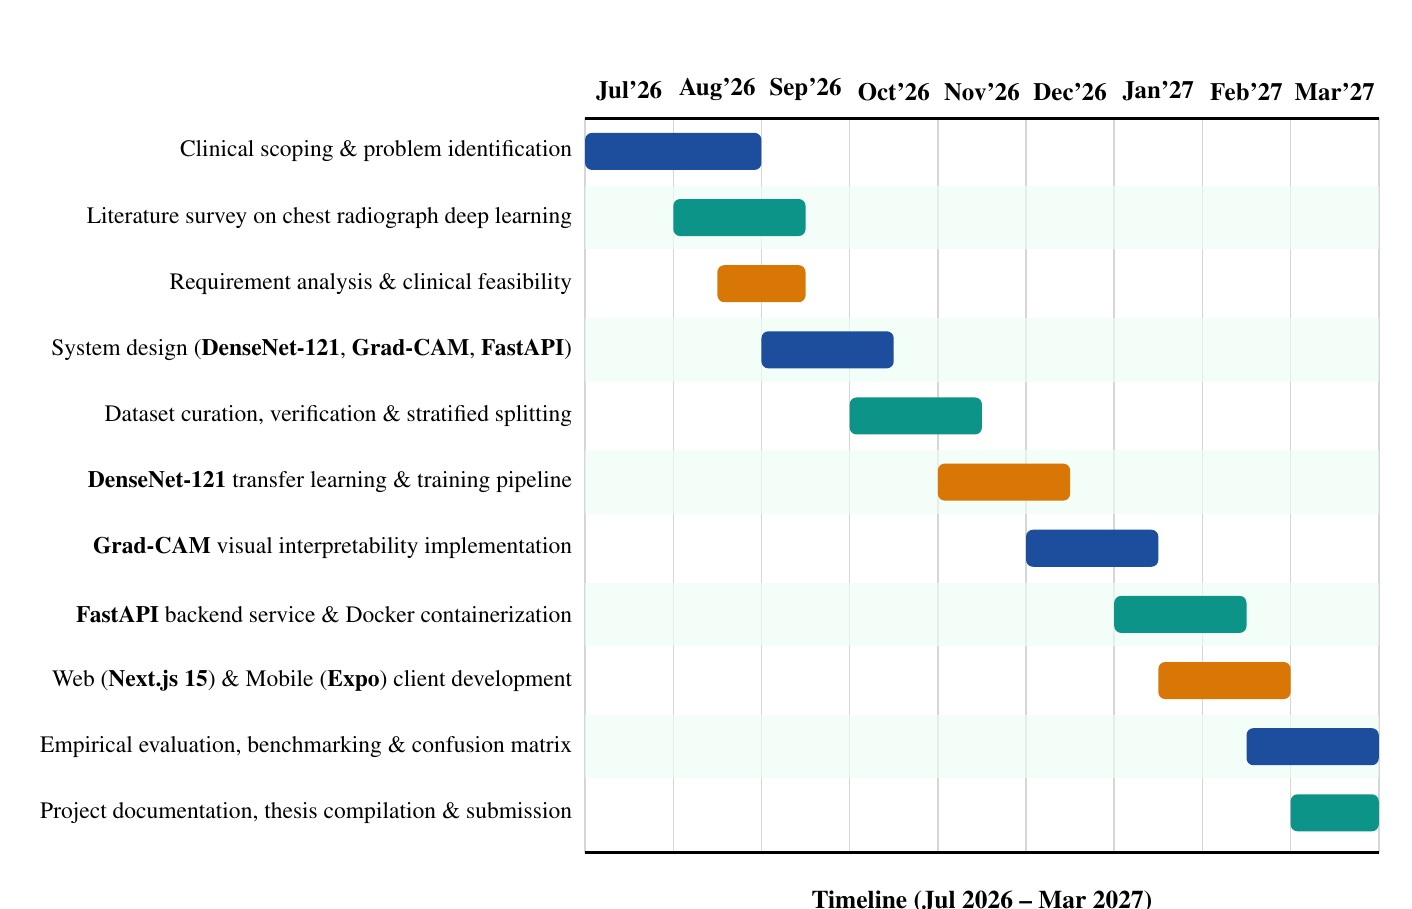
\begin{tikzpicture}[
  x=1.12cm, y=0.84cm,
  lab/.style={anchor=east, font=\fontsize{8.5}{10.5}\selectfont, inner sep=4.5pt, text=black}
]
\def\nm{9}
\def\topY{11.5}

% Vertical month gridlines
\foreach \i in {0,1,...,\nm} {
  \draw[gray!32, line width=0.55pt] (\i, 0.4) -- (\i, \topY);
}

% Month headers on top
\foreach \i/\m in {0.5/Jul'26, 1.5/Aug'26, 2.5/Sep'26, 3.5/Oct'26, 4.5/Nov'26, 5.5/Dec'26, 6.5/Jan'27, 7.5/Feb'27, 8.5/Mar'27} {
  \node[anchor=south, font=\fontsize{9.0}{11.0}\selectfont\bfseries, text=black] at (\i, \topY+0.12) {\m};
}
\draw[black, line width=1.0pt] (0, \topY) -- (\nm, \topY);
\draw[black, line width=0.8pt] (0, 0.4) -- (\nm, 0.4);

% Alternating row background shading
\foreach \k in {0,...,10} {
  \pgfmathsetmacro{\yc}{11.0-\k}
  \ifodd\k
    \fill[prismMint, opacity=0.65] (0, \yc-0.48) rectangle (\nm, \yc+0.48);
  \fi
}

% Task milestone labels on left
\node[lab] at (0, 11.0) {Clinical scoping \& problem identification};
\node[lab] at (0, 10.0) {Literature survey on chest radiograph deep learning};
\node[lab] at (0, 9.0)  {Requirement analysis \& clinical feasibility};
\node[lab] at (0, 8.0)  {System design (\textbf{DenseNet-121}, \textbf{Grad-CAM}, \textbf{FastAPI})};
\node[lab] at (0, 7.0)  {Dataset curation, verification \& stratified splitting};
\node[lab] at (0, 6.0)  {\textbf{DenseNet-121} transfer learning \& training pipeline};
\node[lab] at (0, 5.0)  {\textbf{Grad-CAM} visual interpretability implementation};
\node[lab] at (0, 4.0)  {\textbf{FastAPI} backend service \& Docker containerization};
\node[lab] at (0, 3.0)  {Web (\textbf{Next.js 15}) \& Mobile (\textbf{Expo}) client development};
\node[lab] at (0, 2.0)  {Empirical evaluation, benchmarking \& confusion matrix};
\node[lab] at (0, 1.0)  {Project documentation, thesis compilation \& submission};

% Milestone Gantt Bars
\fill[prismBlue, rounded corners=2.5pt]     (0.0, 11.0-0.28) rectangle (2.0, 11.0+0.28);
\fill[prismTeal, rounded corners=2.5pt]     (1.0, 10.0-0.28) rectangle (2.5, 10.0+0.28);
\fill[prismGold, rounded corners=2.5pt]     (1.5, 9.0-0.28)  rectangle (2.5, 9.0+0.28);
\fill[prismBlue, rounded corners=2.5pt]     (2.0, 8.0-0.28)  rectangle (3.5, 8.0+0.28);
\fill[prismTeal, rounded corners=2.5pt]     (3.0, 7.0-0.28)  rectangle (4.5, 7.0+0.28);
\fill[prismGold, rounded corners=2.5pt]     (4.0, 6.0-0.28)  rectangle (5.5, 6.0+0.28);
\fill[prismBlue, rounded corners=2.5pt]     (5.0, 5.0-0.28)  rectangle (6.5, 5.0+0.28);
\fill[prismTeal, rounded corners=2.5pt]     (6.0, 4.0-0.28)  rectangle (7.5, 4.0+0.28);
\fill[prismGold, rounded corners=2.5pt]     (6.5, 3.0-0.28)  rectangle (8.0, 3.0+0.28);
\fill[prismBlue, rounded corners=2.5pt]     (7.5, 2.0-0.28)  rectangle (9.0, 2.0+0.28);
\fill[prismTeal, rounded corners=2.5pt]     (8.0, 1.0-0.28)  rectangle (9.0, 1.0+0.28);

% Bottom title
\node[font=\fontsize{9.2}{11.2}\selectfont\bfseries, text=black] at (4.5, -0.35) {Timeline (Jul 2026 -- Mar 2027)};
\end{tikzpicture}
\end{document}
}
    \caption{Project execution schedule and Gantt chart tracking 11 key milestones from July 2026 to March 2027.}
    \label{fig:project_gantt}
\end{figure}

The eleven coordinated work packages executed across the academic timeline were:
\begin{enumerate}
    \item \textbf{Clinical Scoping \& Problem Identification (Jul--Aug 2026):} Defined screening boundaries, clinical triage workflows, and diagnostic requirements.
    \item \textbf{Literature Survey on CXR Deep Learning (Aug--Sep 2026):} Reviewed CNN architectures, transfer learning benchmarks, and explainability methods.
    \item \textbf{Requirement Analysis \& Clinical Feasibility (Aug--Sep 2026):} Compiled functional and non-functional specifications and safety bounds.
    \item \textbf{System Design (DenseNet-121, Grad-CAM, FastAPI) (Sep--Oct 2026):} Architected the multi-tier system, component dataflows, and schemas.
    \item \textbf{Dataset Curation, Verification \& Stratified Splitting (Oct--Nov 2026):} Curated multi-class CXR corpora, filtered corrupt files, and split 70/15/15.
    \item \textbf{DenseNet-121 Transfer Learning \& Training Pipeline (Nov--Dec 2026):} Implemented AdamW optimization, augmentations, and early stopping.
    \item \textbf{Grad-CAM Visual Interpretability Implementation (Dec 2026--Jan 2027):} Hooked \texttt{denseblock4} and engineered Jet colormap overlay synthesis.
    \item \textbf{FastAPI Backend Service \& Docker Containerization (Jan--Feb 2027):} Developed asynchronous REST endpoints with MIME and size validation.
    \item \textbf{Web (Next.js 15) \& Mobile (Expo) Client Development (Jan--Feb 2027):} Created drag-and-drop web dashboard and mobile camera film scanner.
    \item \textbf{Empirical Evaluation, Benchmarking \& Confusion Matrix (Feb--Mar 2027):} Evaluated 4,546 test images, achieving 92.63\% accuracy and 98.50\% ROC-AUC.
    \item \textbf{Project Documentation, Thesis Compilation \& Submission (Feb--Mar 2027):} Compiled comprehensive project report and thesis documentation.
\end{enumerate}


%==============================================================================
% CHAPTER 9: CONCLUSION AND FUTURE SCOPE
%==============================================================================
\chapter{Conclusion and Future Scope}

\section{Conclusion}
This project successfully designed, implemented, and empirically evaluated an automated, interpretable deep learning system for \textbf{Early Lung Disease Detection} from chest X-ray radiographs. Addressing the severe clinical challenges of radiologist shortages, diagnostic fatigue, black-box opacity, and workflow deployment barriers, the platform establishes a trustworthy, high-throughput preliminary screening assistant.

The core diagnostic engine leverages transfer learning with \textbf{DenseNet-121}, where direct layer-to-layer feature concatenation maximizes feature reuse and gradient propagation while operating with a compact parameter footprint of only 7.98 million parameters. To ensure clinical auditability, the system embeds \textbf{Grad-CAM} hooked onto \texttt{denseblock4}, generating high-resolution spatial heatmaps that delineate pathological consolidations and ground-glass opacities.

Rigorous evaluation across 4,546 held-out clinical test radiographs confirmed outstanding diagnostic performance, achieving an overall classification accuracy of \textbf{92.63\%}, a macro F1-score of \textbf{91.59\%}, a weighted F1-score of \textbf{92.66\%}, and a One-vs-Rest macro ROC-AUC of \textbf{98.50\%}. Deployed via an asynchronous \textbf{FastAPI} microservice delivering sub-50ms inference alongside responsive \textbf{Next.js 15} web and \textbf{Expo} mobile applications, the platform establishes a practical, point-of-care computer-aided triage tool.

\section{Limitations Encountered}
Despite the strong empirical performance, several technical constraints were encountered:
\begin{itemize}
    \item \textbf{2D Projection Ambiguity:} Chest X-rays represent two-dimensional projections of complex 3D thoracic anatomy, which can occasionally obscure retrocardiac or subdiaphragmatic infiltrates.
    \item \textbf{Class Discrepancy in Severe Pathologies:} Acute viral pneumonia and early-stage COVID-19 can exhibit near-identical bilateral interstitial patterns, occasionally leading to subtle classification overlap.
    \item \textbf{Screening Boundary Constraint:} The system provides preliminary computer-aided triage assistance and cannot replace formal microbiological or RT-PCR confirmatory testing.
\end{itemize}

\section{Future Scope}
Future enhancements to expand and advance the platform include:
\begin{itemize}
    \item \textbf{Multi-Label Co-Morbidity Detection:} Extending the classifier head to detect multiple concurrent pulmonary conditions (e.g., pneumothorax, atelectasis, cardiomegaly, tuberculosis).
    \item \textbf{Volumetric 3D CT Scan Integration:} Incorporating deep learning pipelines capable of analyzing 3D volumetric chest CT scans for high-resolution lesion quantification.
    \item \textbf{Hospital PACS / DICOM Protocol Integration:} Engineering native DICOM network adapters to connect directly with hospital Picture Archiving and Communication Systems (PACS).
    \item \textbf{Federated Multi-Hospital Learning:} Implementing privacy-preserving federated learning protocols enabling model parameter updates across distributed hospitals without sharing private patient radiographs.
\end{itemize}


%==============================================================================
% REFERENCES
%==============================================================================
\begin{thebibliography}{99}
\sloppy

\bibitem{ref_huang2017_densenet}
G. Huang, Z. Liu, L. van der Maaten, and K. Q. Weinberger, "Densely connected convolutional networks," in \textit{Proceedings of the IEEE Conference on Computer Vision and Pattern Recognition (CVPR)}, pp.~4700--4708, 2017.

\bibitem{ref_selvaraju2017_gradcam}
R. R. Selvaraju, M. Cogswell, A. Das, R. Vedantam, D. Parikh, and D. Batra, "Grad-CAM: Visual explanations from deep networks via gradient-based localization," in \textit{Proceedings of the IEEE International Conference on Computer Vision (ICCV)}, pp.~618--626, 2017.

\bibitem{ref_wang2017_chestxray14}
X. Wang, Y. Peng, L. Lu, Z. Lu, M. Bagheri, and R. M. Summers, "ChestX-ray8: Hospital-scale chest X-ray database and benchmarks on weakly-supervised classification and localization of common thorax diseases," in \textit{IEEE CVPR}, pp.~2097--2106, 2017.

\bibitem{ref_rajpurkar2017_chexnet}
P. Rajpurkar, J. Irvin, K. Zhu, B. Yang, H. Mehta, T. Duan, D. Ding, A. Bagul, C. Langlotz, K. Shpanskaya, M. P. Lungren, and A. Y. Ng, "CheXNet: Radiologist-level pneumonia detection on chest X-rays with deep learning," \textit{arXiv preprint arXiv:1711.05225}, 2017.

\bibitem{ref_ozturk2020_covid}
T. Ozturk, M. Talo, E. A. Yildirim, U. B. Baloglu, O. Yildirim, and U. R. Acharya, "Automated detection of COVID-19 cases using deep neural networks with X-ray images," \textit{Computers in Biology and Medicine}, vol.~121, art.~103792, 2020.

\bibitem{ref_apostolopoulos2020_covid}
I. D. Apostolopoulos and T. A. Mpesiana, "Covid-19: Automatic detection from X-ray images utilizing transfer learning with convolutional neural networks," \textit{Physical and Engineering Sciences in Medicine}, vol.~43, no.~2, pp.~635--640, 2020.

\bibitem{ref_he2016_resnet}
K. He, X. Zhang, S. Ren, and J. Sun, "Deep residual learning for image recognition," in \textit{Proceedings of the IEEE CVPR}, pp.~770--778, 2016.

\bibitem{ref_simonyan2014_vgg}
K. Simonyan and A. Zisserman, "Very deep convolutional networks for large-scale image recognition," in \textit{International Conference on Learning Representations (ICLR)}, 2015.

\bibitem{ref_deng2009_imagenet}
J. Deng, W. Dong, R. Socher, L.-J. Li, K. Li, and L. Fei-Fei, "ImageNet: A large-scale hierarchical image database," in \textit{IEEE CVPR}, pp.~248--255, 2009.

\bibitem{ref_shorten2019_augmentation}
C. Shorten and T. M. Khoshgoftaar, "A survey on image data augmentation for deep learning," \textit{Journal of Big Data}, vol.~6, no.~1, art.~60, 2019.

\bibitem{ref_esteva2019_healthcare}
A. Esteva, A. Robicquet, B. Ramsundar, V. Kuleshov, M. DePristo, K. Chou, C. Cui, G. Corrado, S. Thrun, and J. Dean, "A guide to deep learning in healthcare," \textit{Nature Medicine}, vol.~25, no.~1, pp.~24--29, 2019.

\bibitem{ref_topol2019_highperformance}
E. J. Topol, "High-performance medicine: The convergence of human and artificial intelligence," \textit{Nature Medicine}, vol.~25, no.~1, pp.~44--56, 2019.

\bibitem{ref_kelly2019_clinicalai}
C. J. Kelly, A. Karthikesalingam, M. Suleyman, G. Corrado, and D. King, "Key challenges for delivering clinical impact with artificial intelligence," \textit{BMC Medicine}, vol.~17, no.~1, art.~195, 2019.

\bibitem{ref_varoquaux2022_methodology}
G. Varoquaux and V. Cheplygina, "Machine learning for medical imaging: Methodological failures and recommendations for the future," \textit{IEEE Transactions on Medical Imaging}, vol.~41, no.~9, pp.~2434--2444, 2022.

\bibitem{ref_ribeiro2016_lime}
M. T. Ribeiro, S. Singh, and C. Guestrin, ""Why should I trust you?": Explaining the predictions of any classifier," in \textit{ACM SIGKDD International Conference on Knowledge Discovery and Data Mining}, pp.~1135--1144, 2016.

\bibitem{ref_tiwary2022_fastapi}
A. Tiwary and M. Kumar, "Design patterns and performance evaluation of asynchronous microservices using FastAPI," \textit{Software: Practice and Experience}, vol.~52, no.~8, pp.~1802--1821, 2022.

\end{thebibliography}

\end{document}